\documentclass[12pt, twoside]{report}
\usepackage[a4paper,width=150mm,top=25mm,bottom=25mm,bindingoffset=6mm]{geometry}
% \usepackage{bibtex}
\usepackage{minitoc}
\usepackage{amsmath}
\usepackage{fixltx2e}
\usepackage{fancyhdr}
\pagestyle{fancy}
\usepackage[utf8]{inputenc}
\usepackage{tipa}
\usepackage{float}
\usepackage{graphicx}
\usepackage{xcolor}
\usepackage{booktabs}
\usepackage{threeparttable}
\usepackage{pdfpages}
\usepackage{epigraph}
\renewcommand{\textflush}{flushepinormal}
%\usepackage{CJKutf8,bbm}
\usepackage[percent]{overpic}
\definecolor{framboise}{RGB}{143, 0, 55}
\usepackage[breaklinks]{hyperref}
\hypersetup{
  colorlinks=true, %set true if you want colored links
  linktoc=all,     %set to all if you want both sections and subsections linked
  linkcolor=black,  %choose some color if you want links to stand out
  citecolor=framboise
}
\usepackage[hyphenbreaks]{breakurl}
\usepackage{setspace}
%\doublespacing
\usepackage{lineno}

\setcounter{secnumdepth}{3}

\graphicspath{{images/}}

\fancyhead{}
\fancyhead[RO]{\nouppercase{\rightmark}}
\fancyhead[LE]{\nouppercase{\leftmark}}
\fancyfoot{}
\fancyfoot[LE,RO]{\thepage}


\title{
	{Decoding perceptual vowel epenthesis: Experiments \& Modelling}\\
	{\large Institution Name}\\
%	{\includegraphics{university.jpg}}
}
\author{AGR}
\date{Day Month Year}

\begin{document}
\maketitle

\chapter*{Abstract}
Why do people of different linguistic background sometimes perceive the same acoustic signal differently? For instance, when hearing nonnative speech that does not conform to sound structures allowed in their native language, listeners may report hearing vowels that are not acoustically present. This phenomenon, known as perceptual vowel epenthesis, has been attested in various languages such as Japanese, Brazilian Portuguese, Korean, and English. The quality of the epenthesized vowel varies between languages, but also within languages, given certain phonemic environments. 
How much of this process is guided by information directly accessible in the acoustic signal? What is the contribution of the native phonology? How are these two elements combined when computing the native percept? Two main families of theories have been proposed as explanations: two-step and one-step theories. The former advocate an initial parsing of the phonetic categories, followed by repairs by an abstract grammar (e.g., epenthesis), while one-step proposals posit that all acoustic, phonetic, and phonological factors are integrated simultaneously in a probabilistic manner, in order to find the optimal percept.  

In this dissertation, we use a combination of experimental and modelling approaches in order to evaluate whether perceptual vowel epenthesis is a two-step or one-step process. In particular, we investigate this by assessing the role of acoustic details in modulations of epenthetic vowel quality.

In a first part, results from two behavioural experiments show that these modulations are influenced by acoustic cues as well as phonology; however, the former explain most of the variation in epenthetic vowel responses. Additionally, we present a one-step exemplar-based model of perception that is able to reproduce coarticulation effects observed in human data. These results constitute evidence for one-step models of nonnative speech perception.

In a second part, we present an implementation of the one-step proposal in \cite{wilson2013}, using HMM-GMM (hidden Markov models with Gaussian mixture models) from the field of automatic speech recognition. These models present two separate components determining the acoustic and phonotactic matches between speech and possible transcriptions. We can thus tweak them independently in order to evaluate the relative influence of acoustic/phonetic and phonological factors in perceptual vowel epenthesis. We propose a novel way to simulate with these models the forced choice paradigm used to probe vowel epenthesis in human participants, using constrained language models during the speech decoding process.
In a first set of studies, we use this method to test whether various ASR systems with \textit{n}-gram phonotactics as their language model better approximate human results than an ASR system with a null (i.e., no phonotactics) language model. Surprisingly, we find that this null model was the best predictor of human performance. 
In a second set of studies, we evaluate whether effects traditionally attributed to phonology may be predictable solely from acoustic match. We find that, while promising, our models are only able to partially reproduce some effects observed in results from human experiments. Before attributing the source of these effects to phonology, it is necessary to test ASR systems with more performant acoustic models. We discuss future avenues for using enhanced models, and highlight the advantages of using a hybrid approach with behavioural experiments and computational modelling in order to elucidate the mechanisms underlying nonnative speech perception.     

\chapter*{Résumé}
Pourquoi des personnes ayant grandi dans des milieux linguistiques différents ne perçoivent-elles pas toujours un même signal acoustique de la même manière? Par exemple, il arrive que des auditeurs rapportent avoir entendu des voyelles qui n'étaient pas présentes dans l'acoustique de mots non-natifs, lorsque ceux-ci ne se conforment pas aux structures sonores permises dans leur langue. Ce phénomène, connu sous le nom d'épenthèse vocalique perceptive, a été observée dans plusieurs langues telles que le japonais, le portuguais brésilien, le coréen, et l'anglais. L'identité de la voyelle épenthétique varie en fonction des langues, mais aussi parmi les langues elles-mêmes, en fonction des environnements phonémiques.
A quel point ce processus est-il dirigé par des informations directement accessibles dans le signal acoustique ? Quelle est la part de contribution de la phonologie native ? Comment sont combinés ces deux éléments lors du calcul de ce qui est perçu par l'auditeur ? Deux familles principales de théories ont été proposées en tant qu'explications : les théories à deux étapes, et les théories à une étape. Les premières proposent une analyse initiale des catégories phonétiques, suivie de réparations faites par une grammaire abstraite (e.g., cas d'épenthèse). De leur côté, les théories à une étape proposent que tous les facteurs acoustiques, phonétiques, et phonologiques sont intégrés simultanément de manière probabiliste lors du calcul du percept optimal.

Dans cette thèse, nous combinons des approches expérimentales et de modélisation, afin d'évaluer si l'épenthèse vocalique perceptive est un processus à une ou deux étapes. En particulier, nous examinons ceci en mesurant le rôle des détails acoustiques dans les modulations de l'identité de la voyelle épenthétique.

Dans un premier temps, des résultats d'expériences comportementales nous montrent que ces modulations sont influencées aussi bien par les détails acoustiques que par des processus phonologiques. Cependant, la plupart de la variation de l'identité de la voyelle épenthétique est expliquée par l'acoustique. De plus, nous présentons un modèle de perception à une étape qui utilise des exemplaires; celui-ci est capable de reproduire les effets de la coarticulation qui ont été relevés dans les données expérimentales. Ces résultats constituent de l'évidence en faveur des modèles de perception étrangère à une étape.    

Dans un deuxième temps, nous présentons une implémentation du modèle à une étape proposé par \cite{wilson2013}, en utilisant des modèles HMM-GMM (automates de Markov à états cachés en mélanges gaussiens), issus du milieu de la reconnaissance automatique de la parole (RAP). Ces modèles se composent d'un modèle acoustique et d'un modèle de langage, qui déterminent la correspondence acoustique et phonotactique entre la parole et des transcriptions possibles, respectivement. Il nous est alors possible de les ajuster indépendamment afin d'évaluer leur influence relative dans l'épenthèse vocalique perceptuelle. Nous proposons une nouvelle manière d'utiliser ces modèles pour simuler des paradigmes de choix forcés utilisés pour étudier l'épenthèse vocalique chez des participants humains, en utilisant des modèles de language contraints lors du processus de décodage de la parole.

Dans un premier ensemble d'études, nous utilisons cette nouvelle méthode afin de tester si des systèmes de RAP avec des modèles de langage à phonotactique à \textit{n}-grammes donnent des résultats plus proches des résultats humains qu'un système de RAP avec un modèle de langage nul (i.e., sans phonotactique). De manière étonnante, les résultats montrent que le système à modèle de langage nul prédit le mieux la performance des participants.
Dans un deuxième ensemble d'études, nous évaluons si certains effets traditionnellement attribués à des processus phonologiques peuvent être expliqués qu'à partir de la correspondance acoustique. Bien que les résultats soient prometteurs, nos modèles ne sont capables de reproduire qu'une sous-partie des effets observés chez l'humain. Avant de pouvoir attribuer l'origine de ces effets à des processus phonologiques, il est nécessaire de tester des systèmes de RAP avec des modèles acoustiques plus performants. Nous énumérons des futures pistes de recherche d'utilisation de modèles améliorés, et nous soulignons les avantages de l'utilisation conjointe d'expériences comportementales et modélisations computationnelles afin d'élucider les mécanismes sous-jacents la perception de la parole étrangère.  

\chapter*{}
\setlength{\epigraphwidth}{0.9\textwidth}

\epigraph{In general, we look for a new law by the following process: \\ First we guess it. Then we – now don't laugh, that's really true. Then we compute the consequences of the guess to see what, if this is right, if this law that we guessed is right, to see what it would imply. And then we compare the computation results to nature, or we say compare to experiment or experience, compare it directly with observations to see if it works. If it disagrees with experiment, it's wrong. In that simple statement is the key to science. It doesn't make any difference how beautiful your guess is, it doesn't make any difference how smart you are, who made the guess, or what his name is. If it disagrees with experiment, it's wrong. That's all there is to it.}{\textsc{Richard Feynman}}

\epigraph{Los niños han ido con Platero al arroyo de los chopos, y ahora lo traen trotando, entre juegos sin razón y risas desproporcionadas, todo cargado de flores amarillas.
  
  Allá abajo les ha llovido —aquella nube fugaz que veló el prado verde con sus hilos de oro y plata, en los que tembló, como en una lira de llanto, el arco iris—. Y sobre la empapada lana del asnucho, las campanillas mojadas gotean todavía.

  ¡Idilio fresco, alegre, sentimental! ¡Hasta el rebuzno de Platero se hace tierno bajo la dulce carga llovida! De cuando en cuando, vuelve la cabeza y arranca las flores a que su bocota alcanza. Las campanillas, níveas y gualdas, le cuelgan, un momento, entre el blanco babear verdoso y luego se le van a la barrigota cinchada. ¡Quién, como tú, Platero, pudiera comer flores..., y que no le hicieran daño!

    ¡Tarde equívoca de abril!... Los ojos brillantes y vivos de Platero copian toda la hora de sol y lluvia, en cuyo ocaso, sobre el campo de San Juan, se ve llover, deshilachada, otra nube rosa.}{Idilio de Abril. Platero y yo. \\ \textsc{Juan Ramón Jiménez}}

%\chapter*{Declaration}
%I declare that..

\chapter*{Acknowledgements}
I want to thank...
% Reason I feel uncomfortable using a first person pronoun in this thesis is not an attempt of belittling my personal investment in this work, but because of the enormous contribution of a lot of people. I feel like I'm channeling a joint effort, while also taking in as much knowledge myself. 
% do not forget la Maison de la Prairie
% If there was such as thing as more than 2 supervisors: Thomas (corrections, etc, FSTs... There's a frood who really knows where his towel is)!!!! Ewan, Alex Cristia, Page (Paging Dr Page~)!!!! 
% Sanjeev! Hayate!!
% Thanks Emmanuel for believing so much on me finishing this thesis that you made a backup of my consciousness in case a London taxi rolled me over (because of your jaywalking, of course!).
% Les ingénieurs ! Roland, Juan, Mathieu, Julien 
% Thank commité de suivi de thèse (Christophe + David)
% Héctor, Oddur; for reading with outside perspective
% Google team
\chapter*{Publications}

\paragraph{Journal articles}
\begin{itemize}
\item \textbf{Guevara-Rukoz, A.}, Cristia, A., Ludusan, B., Thiollière, R., Martin, A., Mazuka, R., \& Dupoux, E. (2018). \\
  Are words easier to learn from infant- than adult-directed speech? A quantitative corpus-based investigation. \\
  Cognitive Science. https://doi.org/10.1111/cogs.12616
\item Fort, M., Lammertink, I., Peperkamp, S., \textbf{Guevara-Rukoz, A.}, Fikkert, P., \& Tsuji, S. (2018). \\
  SymBouki: a meta-analysis on the emergence of sound symbolism in early language acquisition. \\
  Developmental Science. https://doi.org/10.1111/desc.12659
\item \textbf{Guevara-Rukoz, A.}, Lin, I., Morii, M., Minagawa, Y., Dupoux, E., \& Peperkamp, S. (2017). \\
  Which epenthetic vowel? Phonetic categories versus acoustic detail in perceptual vowel epenthesis. \\
  The Journal of the Acoustical Society of America, 142(2), EL211-EL217.
\end{itemize}
\paragraph{Conference proceedings}
\begin{itemize}
\item \textbf{Guevara-Rukoz, A.}, Parlato-Oliveira, E., Yu, S., Hirose, Y., Peperkamp, S., and Dupoux, E. (2017). \\
  Predicting epenthetic vowel quality from acoustics. \\
  Proceedings of Interspeech, 596-600.
\end{itemize}

%%% Mini TOC %%%
\dominitoc[n]% Initialization
\nomtcrule
%\mtcsetoffset{minitoc}{-4.0em}
\setlength{\mtcindent}{-1.5em}
% % \undotted
\setcounter{minitocdepth}{2}

\tableofcontents
% \linenumbers

\chapter{Introduction}
\setcounter{page}{1}
%%% TO-DO %%%

%%%%%%%%%%%%%%%%%%%%%%%%%%%%%

{\color{red}[Sharon]: I automatically started giving detailed comments, but suddenly realize: why on earth begin your thesis with a story on infants and early acquisition? You should talk about the difficulties adults have perceiving (and if you wish producing) foreign sounds and sound structures! An anecdote would be ok (but not necessary), and then explain that our perception is optimized for native language processing and - if you wish! - that this is put in place during the first year of life.}

Beginning from the time spent in her mother's womb, a baby is exposed to sounds and, importantly, to speech. Initially a ``universal listener'', in her early months she is able to discriminate a wide variety of sounds [CITE]. However, as she is exposed to only one or a few languages that are spoken around her, she progressively loses the ``universal listener'' title. Indeed, through this exposure, her perceptual system progressively becomes attuned to sounds and structures useful for decoding her native language(s) [CITE Werker].

That is, at around 10 months of age, the infant's perceptual system shows signs of becoming optimised for receiving and processing native input.
On the one hand, a native phonemic and suprasegmental inventories are established. Suprasegments are acoustic effects spanning more than one phoneme, such as stress, tone, pitch. But what are phonemes? 
Phonemes, also refer to as segments, are generally defined as the smallest phonetic units capable of conveying a lexical distinction in a language. It is therefore essential for the infant to be able to notice when two different acoustic signals correspond to the same or different phonemes, in order to properly access lexical meaning. For this to happen, her perceptual system partitions the acoustic space into areas corresponding to the phonemes relevant for her native language [CITE]. 

On the other hand, the infant also becomes aware of which phoneme combinations occur in the language and which ones do not [CITE Saffran, ...]. In particular, she progressively acquires the phonotactics for her native language, namely, the constraints determining what constitutes well-formed\footnote{Well-formedness can be defined within a probabilistic framework, but also with hard, binary constraints, or even a combination of the two types of processes. I do not dwell on the subtleties existing between the two in this work, however the interested reader is invited to consult the extensive review in [CITE: Lentz2011].} native sound combinations within words and syllables [CITE: Jusczyk, Pisoni?...]. This is useful, for instance, when trying to find word boundaries in fluent speech, as it is more probable for a rare phoneme combination to occur between words than within words [CITE]. 

Through the optimisation process that results in the acquisition of the native phoneme inventory, native suprasegmentals, and native phonotactics, the infant's perceptual system becomes specialised in her native language, allowing her to better tackle problemes such as word learning.  

Years later, the infant is now an adult with an attuned perceptual system. 
And while this perceptual attunement allows her to communicate efficiently in her native language, issues arise when she now attempts to acquire nonnative languages.
Nonnative speech is processed by her perceptual system, which has been optimised for her native language. The nonnative speech is therefore processed according to her native segmental and suprasegmental inventories, and phonotactics, which do not match those intended by the speech source. 
For our adult listener this will often result in nonnative speech being misperceived; phonemes and prosodic elements might be replaced (assimilation) or deleted (ellipsis). Additional phonemes might even be inserted (epenthesis).

It seems to be generally accepted in the nonnative speech perception literature that misperceptions of nonnative speech result from minimal modifications of the original speech. However, there are multiple proposals relating to the exact nature of these modifications. For instance, are these phonetically-minimal? Phonologically-minimal? At what perceptual stage do they apply? 

Various proposals of mechanisms underlying nonnative speech perception have been put forward; however, many lack formal definition that allow them to be tested empirically.  
In this dissertation, I select one of the proposals advanced by the psycholinguistics literature, namely the perception-based reverse inference models of nonnative speech perception \cite{dupoux2011, wilson2014}, and test a proof-of-concept computational implementation. 
I present various methodologies for qualitatively and quantitatively evaluating the reverse inference proposal, focusing on the phenomenon of perceptual vowel epenthesis.
{\color{red}[Sharon]: ``focus on epenthesis almost goes unnoticed and it's really important!''}
Following on [CITE Peperkamp], the data arising from the computational models is compared to data from psycholinguistics experiments. In these, nonnative speech perception is evaluated using psycholinguistics paradigms which tap onto online (i.e., real-time, individual) perception of nonwords, in order to reduce the influence of confounds such as orthography and semantics.
In other words, I subject the proposed computational models to tasks analogous to those completed by human participants and analyse their behaviour both quantitatively and qualitatively. Do we find perception-based mechanisms to be necessary to predict perceptual vowel epenthesis? If so, do they suffice? 

In order to investigate the underlying mechanisms of nonnative speech perception, we are required to refer to work in two relevant fields, loanword adaptations and nonnative misperceptions.
The former focuses on how words from a source language are modified when introduced to a borrowing language. Rather embedded in the field of theoretical linguistics, this literature offers an indirect window to perception, as loanwords are the product of various complex language transmission phenomena. 
On the other hand, the experimentally inclined literature of psycholinguistics on nonnative speech perception offers more direct data for undestanding misperceptions. However, data may be less readily available than for loanwords. I will now present both literatures, focusing on various mechanisms that have been proposed to explain the phenomenon of vowel epenthesis within both fields.  

{\color{red}[Sharon]: I'd change the order: psycholing. first, and then - because of lack of data - loanwords (which otherwise come out of the blue) \\

Alternatively, if you want to start with loanwords, you should introduce them in the very first paragraph of the intro, which should then go something like this: \\
- we have an accent in L2 \\ 
- we adapt loanwords \\
- both are production phenomena that are at least in part due to speech perception}

\section{Vowel epenthesis in loanword adaptations}
The phenomenon of vowel epenthesis has been studied in the context of loanword adaptations, namely the modification of words from a source language when they are introduced to a borrowing language. Consider the bold vowels in the following examples:
\begin{itemize}
  \item English ``strike'' \textipa{/st\*raIk/} $\rightarrow$ Japanese \textipa{/s\textbf{u}t\textbf{o}raik\textbf{u}/}
  \item French ``baguette'' \textipa{/bagEt/} $\rightarrow$ Japanese \textipa{/baget:\textbf{o}/} %\begin{CJK}{UTF8}{goth}バゲット\end{CJK} \textipa{//} 
  \item English ``snob'' \textipa{/sn6b/} $\rightarrow$ Spanish \textipa{/\textbf{e}snob/}
  \end{itemize}
  
In this context, vowel epenthesis consists in the insertion of a vowel in the (borrowing) surface form of a word that did not contain said vowel in the underlying representation in the source language. Epenthesis often occurs when the introduced word does not respect the phonotactics of the borrowing language (e.g., illegal consonant clusters, illegal syllabification).
The foreign word is imported to the borrowing language in a diachronic process involving multiple individuals and possibly various methods of word transmission (e.g., through written materials, orally, etc). Additionally, adaptations can be influenced by orthography, when available [CITE Daland 2015; Vendelin\&Ppkmp, Ito?]. In this framework the assumption often is that words are introduced to the borrowing language by highly proficient speakers of the source language that are, therefore, able to access a faithful underlying representation of the source word. 

Concerning the question of how the nonnative source word is transformed into the adapted loanword, authors from the loanword literature advance the hypothesis that the underlying mechanisms are phonological and abstract in nature.


{\color{red}Hyman (1970), Lovins (1975), Yip (1993): pre-OT}

For instance, in a grammar-based view, the adapted loanword corresponds to the best match to the source word after candidate adaptations are passed through a grammatical filter  [CITE: Jacobs \& Gussenhoven (2000), Shinohara (2004)]. In this case, {\color{red}[TODO; unclear] the grammar comprises faithfulness and markedness constraints arranged in a certain order, with some authors suggesting that some modifications might be more degrading that others \cite{steriade2001}. How constraints are arranged may or may not be compatible with how native sets of constraints are ordered.} It is assumed that the underlying representation of the source word is accessible and is used in the derivation of the adapted loanword. As such, the faithful underlying representation only becomes adapted when the grammar computes a surface representation from said underlying form (e.g., during production).   \\

Another similar mechanism was proposed by [CITE La Charité \& Paradis (2005)], where adaptations are based on minimal featural changes. The source word is adapted by highly proficient bilinguals, who can manipulate and compare the phonological systems of both the source and the borrowing languages. In this case, adaptation consists in these highly proficient bilinguals choosing the modifications of the source word that result in the least featural changes between the source adaptation and the resulting loanword.  

In many proposals, the role of perception has been assumed to be minimal, or at least secondary, in loanword adaptation [CITE e.g., LaChParadis1997]. However, this view is far from being a consensus. For instance, as briefly mentioned earlier, \cite{steriade2001} proposed that some grammar-based modifications resulted in more perceptually-salient modifications of the source word, resulting in a greater amounts of degradation.
Also, [CITE silverman1992] proposed his multiple scansion theory of loanword adaptation. In this theory, the underlying representation in the borrowing language is retrieved from a phonetic, possibly acoustic, form of the source word. In a first step, a perceptual-level representation is established, where the underlying representation is built with preliminary segmental and prosodic structure. It is only at a second step, at the operational level, that the phonology of the borrowing language is applied to the word (e.g., through a grammatical filter), resulting in modifications such as vowel epenthesis, when necessary. For similar proposals, see [CITE Kenstowicz 2001/2003, KenstowiczSuchato, Yip1993/2006].  

{\color{red}Alternative structure: Change to (1) Purely phonological and (2) Perceptual}


\section{Perceptual vowel epenthesis}

In the late nineties various theories of nonnative speech perception [CITE Best1995, Kuhl1995] and second language phoneme acquisition [Flege1995] surfaced in the psycholinguistics literature. There seemed to be an overlap between the observed nonnative speech misperceptions and patterns observed in loanwords; may perception directly account for loanword adaptation?   
It is in this context that appeared proposals such as that of [CITE PeperkampDupoux2003], which put greater emphasis on the role of misperception on loanword adaptation. The proposal being that, when perceiving nonnative input, a phonetic decoding module takes into account segmental, suprasegmental, and syllabic inventories of the native language in order to derive a phonetically-minimally modified representation\footnote{Whether this representation is acoustic, articulatory [CITE cf Berent2015], and/or gestural [CITE: BrowmanGoldstein, Best1995, BestTyler2007] in nature is not discussed here.} of the acoustic input. It is this misperceived version that is then converted into an underlying representation by a phonological decoding module; this cemented underlying representation is unfaithful with respect to the original underlying representation in the nonnative language.  
% As mentioned above epenthesis is the phenomenon in which a sound that was not initially present in the input is inserted and surfaces in the output\footnote{Depending on context, the word ``epenthesis'' can refer to the addition of any sound (consonant, vowel ...) in different situations such as online perception, online production, diachronic lexical changes, etc. For the purpose of this thesis, however, we will specifically use the word ``epenthesis'' to refer to perceptual vowel epenthesis, unless stated otherwise.}.
In this context, when listeners experience perceptual vowel epenthesis, they hallucinate vowels not initially present in the nonnative speech. In the cases studied in this work, this happens as a way to break phonotactically illegal clusters. For instance, in Japanese most consonant clusters%\footnote{Consonant clusters can only be geminates or a nasal followed by another consonant.}
, such as \textipa{/bz/}, are phonotactically illegal. When hearing nonwords containing these clusters, such as \textipa{/ebzo/}, Japanese listeners may hallucinate an epenthetic \textipa{/u/}\footnote{A more accurate phonetic transcription of the unrounded high back vowel used in Japanese is \textipa{[W]} but, following previous work, the phonological notation \textipa{/u/} will be used in the remainder of the thesis.} within the cluster, yielding \textipa{/ebuzo/} as the percept \cite{dupoux1999}. Epenthesis of \textipa{/u/} by Japanese listeners is not only evident in their behaviour but also in their brain responses; they have difficulties differentiating the clusters produced by a French speaker from their epenthesized counterparts (e.g., \textipa{/ebzo/} \textit{vs.} \textipa{/ebuzo/}) while also showing different event-related potentials compared to native French speakers. The fact that Japanese listeners fail to show sign of MMN (mismatch negativity) in the EEG signal attests that the process of epenthesis occurs early in the process of perception \cite{dehaene2000}. Importantly, experimental data also suggests that epenthesis is a pre-lexical process happening early in speech perception \cite{dupoux2001}.
Epenthesis has also been attested in languages other than Japanese [cite: Dupoux (1999), Dehaene-Lambertz (2000), Dupoux (2001), Monahan (2009), Dupoux (2011), Mattingley (2015)]; it has also been studied in languages such as Korean [cite: de Jong \& Park (2012), Durvasula (2015), Shin \& Iverson (2011)], Brazilian Portuguese [cite: Dupoux (2011)], Spanish [cite: Hallé (2014), Daland], English [cite: Berent (multi), Davidson], and Mandarin Chinese [cite: Durvasula (2018)].

While research on perceptual vowel epenthesis uses the literature on loanword adaptation as a a source of inspiration and a source of informed predictions, it is important to note that the phenomenon of vowel epenthesis is not defined equally in both fields. Remember that loanword adaptation is a diachronic process, involving complex interactions between several groups of individuals, with varying degrees of source language fluency. 
In contrast, the psycholinguistic approach focuses on online perception and, while data from multiple participants is collected, the modifications observed on the output of perception are assumed to occur at the level of the individual, as there is no interaction between participants. Participants are not expect to be proficient in the nonnative language, which minimises the influence of linguistic knowledge on misperceptions (e.g., orthography). 

%  - Shin \& Iverson (2011): correlation between \%epenth and vowel discrimination.   \\
% - Kabak \& Idsardi (2007): a phonological influence of L1 phonotactic knowledge, rather than an effect of frequency, plays a primary role in explaining KR groups performance."
%- Browman \& Goldstein (1980s): Articulatory Phonology; dynamic gestures as units, developing in space at time (as opposed to the static segment). Sounds correspond to constellation of gestures. Allows to explain gradient effects.  
%- Zhao \& Berent (2018): Epenthesis from read stimuli (i.e., no acoustic input) \\
%- Best \& Tyler (2007): "PAM posits that perceivers extract invariants about *articulatory gestures* from the speech signal, rather than forming categories from acoustic-phonetic cues"

\section{Processing steps in perceptual vowel epenthesis}

From now on we will focus on perceptual vowel epenthesis, referring to loanwords as a source of inspiration for experimental setups and as a source of informed predictions. Concerning the process of vowel epenthesis, we can identify two types of proposed pipelines that differ in the amount of processing steps that the nonnative input is subjected to during perception: these are two-step and one-step theories of nonnative speech perception, illustrated in Figure \label{ref:intro_12step}. While these names are somewhat transparent, we will now explain in more detail the differences between the two types of proposals.   

Reminiscent of Silverman's multiple scansion theory for loanword adaptations \cite{silverman1992}, two-step theories of nonnative speech perception divide the perception process in two stages. According to these proposals, the quality of the epenthetic vowel is determined by a language-specific grammar after an initial parsing of the nonnative input.
For \cite{berent2007}, the identity of the segments present in the nonnative input is retrieved in an initial step, yielding a \textit{phonetic form}. The native grammar then assesses the phonotactic legality of this phonetic form in a second step. If a phonotactic violation is found, the grammar, which combines both language-specific and universal components, repairs the phonetic form by inserting a vowel. The output of this final step is the \textit{phonological representation}.
Another proposal, that of \cite{monahan2009}, also consists in two steps, but with some differences. During the first step the identity of the segments in the input is retrieved and segments are grouped into syllables, following native phonotactics. Some syllables will contain indeterminate segments (e.g., \textipa{/ebzo/} will have been parsed as \textipa{/e.b}V\textipa{.zo/}). In a second step, the quality of the indeterminate segments, in this case the epenthetic vowel, is chosen amongst vowels that are of low sonority and can undergo devoicing. {\color{red}[Sharon]: ``explain low sonority and especially give background on vowel devoicing''}
The quality of the vowel might not be determined if an optimal match is not found.
The two proposals that we have summarised share the fact that the categorisation of the segments that are not the epenthetic vowel occurs in a first step and it is not modified during the second step, where the identity of the epenthetic vowel is determined.

\begin{figure}[htb!]
  \centering
  \begin{overpic}[page=1, width=0.9\linewidth]{chapter01-intro/12step}\end{overpic}
  \caption{\textit{Processing of the nonnative stimulus \textipa{/ebzo/} by Japanese listeners, according to two-step and one-step proposals for perceptual vowel epenthesis. {\color{red}[Sharon]: Add citations for reverse inference as well.}}}
  \label{fig:intro_12step}
\end{figure}

In contrast, with one-step proposals, authors such as \cite{dupoux2011} and \cite{wilson2013} argue that the identity of the epenthetic vowel is determined in the process of parsing the input, simultaneously to the categorisation of all other segments. The phonotactic legality of the input is therefore assessed at the same time as the categorisation happens. Notably, the input is not processed as a linear sequence of sounds; syllabic structure is taken into account during the parsing process \cite{kabak2007}.

\cite{wilson2013} qualify the process as a process of reverse inference within a Bayesian framework, where the perceptual system computes $P(w | X)$ the posterior probability of candidate percepts $w$ given the auditory input $X$. These are estimated, for each candidate percept, from the product of $P(X|w)$ the likelihood of the acoustics given the percept and $P(w)$ the prior probability of the percept, defined as its phonotactic acceptability. Mathematically, this can be formulated as in equation \ref{eq_onestep1}. Then, in a maximum \textit{a posteriori} (MAP) estimation scenario, the final percept $\widehat{w}$ corresponds to the percept with the highest posterior probability, as shown in equation \ref{eq_onestep2}. Alternatively, the final percept may be estimated by weighted sampling, where weights are defined by the posterior probabilities.     

\begin{equation}
  P(w | X) \propto P(X | w) \cdot P(w)
  \label{eq_onestep1}
\end{equation}

\begin{equation}
  \widehat{w} = \underset{w}{arg\,max} \left \{ P(X|w) \cdot P(w) \right \}
  \label{eq_onestep2}
\end{equation}

In other words, for one-step models, parsing becomes an optimisation problem where the optimal output is the one maximising the acoustic match to the input and the likelihood of the phonemic sequence in the native language. \cite{durvasula2015} adds to the aforementioned proposals by suggesting that listeners are decoding nonnative speech through a {\color{red}process of reverse inference that not only optimises the output according to phonetic representations and surface phonotactics, but also according to native phonological alternations (i.e., mappings between underlying and surface representations) [Sharon]: clarify.}.

\section{Justifying the modelling approach}
\epigraph{... But why make models?}{\textit{Derek Zoolander, probably.}}

{\color{red}[Sharon]: ``cette section est très courte. Ne peux-tu pas donner une synthèse historique sur l'utilisation de la modélisation en perception de la parole (ou, su tu veux, perception en général, psychophysique, qu'en sais-je...)''}

In this thesis I will evaluate computational implementations of one-step theories of nonnative speech perception. Notably, I will investigate models from the field of automatic speech recognition (ASR) which are a direct implementation of the Bayesian model shown in equation \ref{eq_onestep1}\footnote{The equivalent of a weighted sampling procedure was preferred over MAP estimation for percept selection, since participant responses in previous experimental work on epenthesis tended to show variation and were not deterministic.}. 
While only the one-step family of theories will be evaluated in this work, I encourage further research to be done with similar methodologies in order to investigate all of the various co-existing proposals.

Indeed, using computational models in order to investigate competing theories is beneficial in several ways. Firstly, the need to translate the theories into model implementations forces model ideators to provide a mathematically and/or algorithmically well defined model. This is in contrast to more vague and ambiguous verbally defined theories that leave more space to reader interpretations. Having more rigorous model definitions also allows for a better understand competing theories (what is the exact nature of the input? which grammar constraints are applied and how? ...), meaning that it is easier to compare proposals and see where they differ significantly or not. 

Secondly, obtaining a computational implementation of a theory means that it is then possible to derive predictions from the models in question. It is then possible to qualitatively and quantitatively examine these predictions, and compare them to what is observed in behavioural data.

\section{Outline of this thesis}
%%%%%%%

{\color{red}[TO-DO while writing discussion]}





\chapter{Role of acoustic details in the choice of epenthetic vowel quality}
\minitoc
%%%%%%%%%%%%%%%%%%%%%%
% Chapter mini-intro %
%%%%%%%%%%%%%%%%%%%%%%
\newpage
\section{Introduction}
As presented in the Introduction, work on loanword adaptation and online speech perception shows that listeners epenthesize or delete vowels from nonnative input when it does not conform to native non-native phonotactics.
While this statement seems to be generally accepted, the mechanisms underlying these phenomena are subject to more debate. In this chapter we will investigate the mechanisms underlying variations of epenthetic vowel quality. 


\subsection{One-step vs two-step theories}

We saw that theories such as those by \cite{berent2007, monahan2009} view perceptual vowel epenthesis as a two-step process.
According to these proposals, the quality of the epenthetic vowel is determined by a language-specific grammar after an initial parsing of the nonnative input.
In contrast, one-step theories such as those proposed by \cite{dupoux2011, dejong2012, wilson2013, durvasula2015} argue that parsing is an optimisation problem where the optimal output maximises the acoustic/phonetic match to the input and the likelihood of the phonemic sequence in the native language. 

How can we confront and test these one-step and two-step proposals? For this, we can dissect the phenomenon of perceptual vowel epenthesis and split it into two subproblems:
\begin{enumerate}
    \item When does epenthesis occur?
    \item What vowel is epenthesized?
\end{enumerate}
    
Concerning the first subproblem, neither one-step theories nor two-step theories give explicit predictions concerning the rate of epenthesis. It is even unclear if the two-step theories exposed above allow for epenthesis to \textit{not} happen. In the case of \cite{berent2007}, not epenthesizing a vowel would require directly yielding the phonetic form, without repairs being performed by the grammar. While \cite{berent2007} hypothesizes that this may happen in tasks requiring participants to pay more attention to phonetics, it is unclear in which cases listeners would directly retrieve the phonetic form within a same task, for similar stimuli. In the case of \cite{monahan2009}, lack of epenthesis would involve a different syllabification of the input than when epenthesis happens. Therefore, a priori, epenthesis should always happen if the input is syllabified according to native phonotactics. In the case of reverse inference one-step theories \cite{dupoux2011, dejong2012, wilson2013, durvasula2015}, lack of epenthesis might occur if the optimal match between the nonnative input and the native output is more strongly driven by acoustic/phonetic match than by sequence acceptability.   

We now turn to the second subproblem, epenthetic vowel quality. For a given phonemic sequence containing a phonotactic violation, two-step theories would predict that epenthetic vowel quality is determined after an initial categorisation step. As such, we do not expect different tokens of a same type to yield epenthetic vowels of different quality. On the other hand, this would be possible for one-step accounts, since the acoustic details are included in the computation of the optimal output. Examining modulations in epenthetic vowel quality, therefore, allows to empirically tease apart one-step and two-step theories summarised above.      

\subsection{Role of acoustics}
Results by \cite{dupoux2011} support one-step theories, since the authors were able to modulate the identity of the epenthetic vowel perceived by Japanese and Brazilian Portuguese listeners from stimuli that had the exact same segmental structure. For instance, Japanese listeners could be let to epenthesize \textipa{/i/} more often instead of their default \textipa{/u/} within consonant clusters (and vice versa for Brazilian Portuguese listeners). What are the factors determining whether participants more readily epenthesized \textipa{/i/} or \textipa{/u/}?

The modulations in epenthetic vowel quality observed in \cite{dupoux2011} were due to acoustic cues present in the stimuli. Stimuli with the same segmental sequence were constructed by excising the medial vowel from \textipa{/ebuzo/} and \textipa{/ebizo/}, yielding \textipa{/eb(u)zo/} and \textipa{/eb(i)zo/}. These items differ in the coarticulation cues remaining in the consonants, but they have identical segmental structure (\textipa{/ebzo/}). Participants epenthesized \textipa{/i/} more often from \textipa{/eb(i)zo/} than from \textipa{/eb(u)zo/}, and similarly for \textipa{/u/}.

Remember that, for the two-step proposals above, the quality of the epenthetic vowel is determined in a second step, after the identity of the segments has been blocked. Both \textipa{/eb(u)zo/} and \textipa{/eb(i)zo/} would have \textipa{/ebzo/} as a phonetic form (following \cite{berent2007}) or they would be parsed as \textipa{/e.b}V\textipa{.zo/} (following \cite{monahan2009}). We cannot predict the modulations in epenthetic vowel from these initial parsings. However, in a one-step processing the acoustic details (in this case, coarticulation) could be taken into account when computing the acoustic match between the input and possible output phoneme sequences. 

In this view, the representation used as input for the computation is acoustic in nature. This is in contrast to proposals of input as featural representation (e.g., binary, geometric). For instance, it has been hypothesized that the phenomena of epenthetic vowel copy (i.e., when the epenthetic vowel shares quality with neighbouring vowels) is due to a transfer of phonological features from neighbouring vowels and/or consonants towards an undeterminate epenthetic vowel \cite{rose2006, uffmann2006}. These phonological explanations of epenthetic vowel quality would therefore predict that, in auditory stimuli where the quality of the coarticulation and the quality of neighbouring vowels would be in conflict, the quality of the epenthetic vowel would mostly be determined by the neighbouring vowels.      

\subsection{Chapter preview}

In this chapter we will investigate perceptual vowel epenthesis in order to tackle three main questions: 

%% Research questions %%
\begin{itemize}
\item How does the influence of acoustic details on epenthetic vowel quality compare to other influences such as those of an abstract grammar?
\item Stimuli in \cite{dupoux2011} were made by excising vowels. Can we reproduce the modulations of epenthetic vowel quality caused by coarticulation using naturally produced stimuli?
\item And finally, if acoustic factors are essential when choosing epenthetic vowel quality, does this mean that they are sufficient to do so?
\end{itemize}

In \textbf{section \ref{2-ahpa}} a perceptual experiment aims at disentangling the contributions of phonetic categories and acoustic details on epenthetic vowel quality. Participants are asked to report their choice of epenthetic vowel (if any) within consonant clusters in stimuli where the acoustic information contained in the cluster may be in disagreement with the identity of neighbouring vowels. Information theoretic measures allow us to quantify the influence of both neighbouring phonetic categories and acoustic details.

In \textbf{section \ref{2-parlato}} we explore the possibility of predicting epenthetic vowel quality in Brazilian Portuguese (BP) and Japanese (JP) using a production-based exemplar model of perception. This type of model predicts the quality of a vowel epenthesized within the cluster of a stimulus based solely on the acoustic similarity of said /CC/ cluster to /CVC/ exemplars produced by native speakers of BP or JP. From this modelling approach we can evaluate the influence of pure acoustics on effects such as default epenthetic vowel quality and modulations induced by neighbouring vowels, with naturally produced stimuli that have not been manipulated.

In \textbf{section \ref{2-parlato-dur}} we modify the production-based exemplar models from section \ref{2-parlato}. Several modifications are applied, mostly based on increased performance during the parameter optimisation phase. However, a notable modification is the normalisation of features by speaker (our input is still acoustic in nature, but it is closer to phonetics than previously). Also, we include in our models the possibility to add a duration-mismatch penalty, based on the finding that default epenthetic vowels are also those that are shorter. We examine the effect of the presence or absence of the duration penalty on default epenthetic vowel choice and modulations of epenthetic vowel quality by neighbouring vowels.   

%%%%%%%%%%%%%%%%%%%%
% /ahpa/ (JASA-EL) %
%%%%%%%%%%%%%%%%%%%%

\newpage
\section{Which epenthetic vowel? Phonetic categories versus acoustic detail in perceptual vowel epenthesis} \label{2-ahpa}

\small{\textit{{\color{darkgray}The following section is a modified version of the following journal article: \\
Guevara-Rukoz, A., Lin, I., Morii, M., Minagawa, Y., Dupoux, E., \& Peperkamp, S. (2017). Which epenthetic vowel? Phonetic categories versus acoustic detail in perceptual vowel epenthesis. Journal of the Acoustical Society of America, 142(2), EL211-EL217. \\
Stimuli were designed and recorded by I. Lin.
Experimental data for the identification task were collected by M. Morii and Y. Minagawa, using scripts by A. Guevara-Rukoz. The ABX experiment was designed and run by I. Lin.
Statistical analyses, phonetic transcriptions, and acoustical analyses were performed by A. Guevara-Rukoz.
The initial manuscript draft was prepared by E. Dupoux, S. Peperkamp, and A. Guevara-Rukoz.
E. Dupoux and S. Peperkamp supervised the entirety of the study.\\
Modifications with respect to the original paper: additional figures, annexes.\\}}}
%{\color{red}Note to Sh \& Emm: please correct acknowledgements if wrong.}
\paragraph{Abstract}

This study aims to quantify the relative contributions of phonetic categories and acoustic detail on phonotactically-induced perceptual vowel epenthesis in Japanese listeners. A vowel identification task tested whether a vowel was perceived within illegal consonant clusters and, if so, which vowel was heard. Cross-spliced stimuli were used in which vowel coarticulation present in the cluster did not match the quality of the flanking vowel. Two clusters were used, /hp/ and /kp/, the former containing larger amounts of resonances of the preceding vowel. While both flanking vowel and coarticulation influenced vowel quality, the influence of coarticulation was larger, especially for /hp/.

\subsection{Introduction}
% \label{sec:Introduction}

\setlength{\parindent}{5ex}

Our auditory perceptual system is tuned to the sound system of our native language, resulting in impoverished perception of nonnative sounds and sound sequences \cite{sebastian2005}. For instance, in Japanese, a vowel can only be followed by a moraic nasal consonant or by a geminate consonant. As a consequence, Japanese listeners tend to perceive an illusory, epenthetic, \textipa{/u/} within illegal consonant clusters \cite{dupoux1999, dehaene2000, dupoux2001, monahan2009, dupoux2011, guekozIS17} and it is evident in loanword adaptation as well (e.g. the word 'sphynx' is borrowed in Japanese as /sufiNkusu/). Similar effects have been documented in other languages, with different epenthetic vowels (\textipa{/1/} in Korean \cite{kabak2007, berent2008, dejong2012}; schwa in English \cite{berent2007, davidson2012}; /i/ in Brazilian Portuguese \cite{dupoux2011, guekozIS17}; and /e/ in Spanish \cite{halle2014}). Even within languages, there sometimes is variation in the quality of the epenthetic vowel; for instance, in Japanese, the epenthetic vowel can in certain contexts be \textipa{/i/} or \textipa{/o/} \cite{mattingley2015, guekozIS17}.

The factors that determine the quality of the epenthetic vowel are still unclear. There is evidence that local acoustic cues in the form of vowel coarticulation play a role. Specifically, using artificial consonant clusters obtained by completely removing an inter-consonantal vowel, \cite{dupoux2011} found that the quality of the removed vowel -- traces of which are present in the neighboring consonants -- influences the quality of the epenthetic vowel. Other studies, however, have argued for an influence of phonological factors, such as the legality of the resulting repair at the phonotactic level \cite{mattingley2015} or the presence of phonological alternations in the language \cite{durvasula2015}. Determining the source of epenthetic vowel quality is important at a theoretical level, because it can shed light on the computational mechanisms underlying the perception of speech sounds. For instance, \cite{dupoux2011} argued that coarticulation effects cannot be accounted for by two-step models, in which the repair of illegal sequences follows that of phoneme categorization, while they are in accordance with one-step models, in which phoneme categorization takes phonotactic probabilities into account.
\footnote{Note that due to a typo the summary in the first-to-last paragraph of this article erroneously states the opposite.} 
However, \cite{dupoux2011} only assessed the presence of acoustic effects, without investigating a possible role of categorical effects. Here, our aim is to quantify the relative contributions of categorical and acoustic effects on epenthetic vowel quality by directly comparing these two types of effect. 

We focus on perceptual vowel epenthesis following \textipa{/h/}. This case is ideally suited for our objective as in Japanese loanwords these fricatives are typically adapted by adding a `copy' of the preceding vowel when they occur in a syllable coda. For instance, \textit{`Bach'}, \textit{`(van) Gogh'}, and \textit{`Ich-Roman'} are adapted as \textipa{/bah:a/}, \textipa{/goh:o/}, and \textipa{/ih:iroman/}. In work on loanword adaptations, cases of vowel copy in epenthesis have been explained as a result of the spreading of phonological features from the preceding vowel onto the epenthetic vowel (i.e., vowel harmony), for instance in Shona, Sranan, and Samoan \cite{uffmann2006}, and Sesotho \cite{rose2006}. In speech perception, however, this pattern could be based either on phonetic categories, i.e. the preceding vowel itself, or on acoustic detail, i.e. traces of this vowel that are present in /h/, as laryngeal fricatives such as \textipa{/h/} contain acoustic information relative to formants of surrounding vowels \cite{keating1988}. Using an identification task, we tease apart these two explanations by independently manipulating the categorical context in which \textipa{/h/} occurs and the acoustic realization of this segment, using cross-splicing. As a control, we also use stimuli with \textipa{/k/}, which are expected to give rise to more default \textipa{/u/}-epenthesis because they contain less coarticulation. 

\subsection{Methods}

\subsubsection{\textit{Participants}}
%\label{ssec:subj}

Twenty-five native Japanese speakers were tested in Tokyo, Japan (mean age $24 \pm 3.5$; 13 female). All were students at Keio University, and none had lived abroad. 

\subsubsection{\textit{Stimuli}}
%\label{ssec:stim}

We constructed a set of 20 base items, 10 disyllabic ones of the form $V_{1}C_{1}C_{2}V_{1}$ and 10 matched trisyllabic ones of the form $V_{1}C_{1}V_{1}C_{2}V_{1}$, 
with $V_{1}$ a vowel in the set \textipa{/a, e, i, o, u/} (henceforth: flanking vowel), $C_{1}$ \textipa{/h/} or /k/, and $C_{2}$ a fixed consonant, /p/, e.g. \textipa{/ahpa/}, \textipa{/ekpe/, /ohopo/, /ikipi/}. Three trained phoneticians, native speakers of Dutch, American English and Argentinian Spanish, respectively, recorded all items with stress on the first syllable. All /kp/ stimuli presented release bursts. For each disyllabic item, we used one token per speaker as a natural control stimulus. By systematically replacing the $/C_{1}C_{2}/$-cluster in these items by the same cluster out of the other disyllabic items produced by the same speaker but with a different vowel, we created spliced test stimuli such as $/ah_{o}pa/$, and $/ek_{i}pe/$, where the small vowel denotes vowel coarticulation present in the consonant cluster. Similarly, by replacing the $/C_{1}C_{2}/$-cluster in the disyllabic items by the same cluster out of the second token of the same items, we created spliced control stimuli in which the vowel coarticulation matched the flanking vowel, e.g. $/ah_{a}pa/$, $/ek_{e}pe/$. We also created trisyllabic fillers in which the middle vowel either matched or mismatched the flanking vowel, e.g. \textipa{/ahapa/}, \textipa{/ekepe/}, \textipa{/ahopa/}, \textipa{/ekipe/} (these were also created by splicing, as they served as test stimuli in an experiment not reported in this article). Overall, each speaker thus contributed 40 test stimuli (5 flanking vowels x 4 vowel coarticulations x 2 consonant clusters), 20 control stimuli (5 flanking vowels x 2 consonant clusters, all both in a natural and a spliced form), and 50 fillers. Ten additional training items were recorded by a fourth speaker. Their structure was similar, but included only phonotactically legal nasal + stop sequences with or without an intervening copy vowel (e.g., \textipa{/ampa/, /enepe/}). 

\subsubsection{\textit{Procedure}}
%\label{ssec:procedure}

Participants were tested individually in a soundproof room. At each trial, they heard a stimulus over headphones and were asked to identify the vowel between the two consonants, if any. They were provided with a transcription of the item on screen, containing a question mark between the two consonants (e.g. \textit{``ah?pa"}) in latin characters (as non-CV syllables cannot be transcribed using Japanese characters), as well as the list of possible responses: \textit{``none, a, i, u, e, o"}. Participants responded by pressing labelled keys on a keyboard. Participants were familiarised with the procedure with 10 training trials in which they received on-screen feedback. 

The 330 stimuli were presented in a pseudo-randomised order: Consecutive stimuli were produced by different speakers, and a stimulus could not be followed by a stimulus with the same combination of vowel coarticulation and consonant. Trials were presented in two blocks, with each stimulus appearing once per block, for a total of 660 trials. The experiment lasted approximately 40 minutes. 

\subsection{Results}
%\label{sec:results}

Test and control trials with responses that were either too fast (before the medial portion of the stimulus could be perceived and processed, $<$400 ms) or too slow ($>$ 3 SD: 3238 ms) were excluded from the analyses. This concerned 736 trials (4.5\%).

\subsubsection{\textit{Control items}}
% \label{ssec:ctrl_items}

Participants experienced perceptual epenthesis in 57\% of control items in which the flanking vowel and coarticulation are of the same quality (/hp/: 52\%, /kp/: 61\%). Recall that in loanwords, the default epenthetic vowel is /u/, while after voiceless laryngeal fricatives it is a copy of the preceding vowel. Focusing on trials with an epenthetic response, we examined whether the choice of epenthetic vowel reflected this pattern.

\begin{figure}[htb!]
  \centering
  \begin{overpic}[page=1, width=0.45\linewidth]{chapter02/ahpa_uep-copyep}\end{overpic}
  \hspace{0.5cm}
  \begin{overpic}[page=2, width=0.45\linewidth]{chapter02/ahpa_uep-copyep}\end{overpic}
  \caption{\textit{Percentage of default /u/-epenthesis (left) and vowel copy epenthesis (right) for control items. Box plots display the distribution of the scores across speakers (median, quartiles and extrema), with gray lines connecting data points corresponding to a single participant.}}
  \label{fig:ahpa_uep-copyep}
\end{figure}

First, a generalised mixed-effects model with a declared binomial distribution \cite{R-lme4} was used to examine a possible effect of consonant cluster on default /u/-epenthesis. Thus, we analyzed the proportion of default \textipa{/u/}, using participant, speaker, experimental block, and trial as random effects, and consonant cluster (\textipa{/kp/} \textit{vs.} \textipa{/hp/}; contrast coded) as fixed effect. This model was compared to a reduced model with no fixed effect. The full model was found to explain significantly more variance than the reduced model ($\beta = -4.2$, $SE = 1.2$, $\chi^{2}(1) = 9.9$, $p < 0.01$), showing that participants experienced significantly less default /u/-epenthesis in \textipa{/hp/-} than \textipa{/kp/-}items (39\% \textit{vs.} 86\% of all trials with epenthesis, respectively). 

Next, we examined whether epenthesized vowels shared the quality of the flanking vowel more often in /hp/- than in /kp/-clusters. Given that for items with flanking vowel /u/ it is impossible to know if /u/-epenthesis is due to vowel copy or to default epenthesis, these items were excluded. As before, a generalised mixed-effects model with a declared binomial distribution was used. We analyzed the proportion of vowel copy (i.e., whether the flanking vowel and epenthetic vowel shared quality), using participant, speaker, experimental block, and trial as random effects, and consonant cluster (\textipa{/kp/} \textit{vs.} \textipa{/hp/}; contrast coded) as fixed effect. Comparing this full model to a reduced model with no fixed effects revealed a significant effect of consonant cluster ($\beta = 3.7$, $SE = 1.2$, $\chi^{2}(1) = 7.4$, $p < 0.01$). Therefore, participants epenthesized a vowel that matched the flanking vowel more often in /hp/-clusters ($53\%$) than in /kp/-clusters ($13\%$). 

Thus, analysis of control items revealed that, similarly to the loanword pattern, participants perceived the vowel /u/ more often in /kp/- than in /hp/-clusters, and they perceived a vowel copy more often in /hp/- than in /kp/-clusters.

\subsubsection{\textit{Test items}}
\label{ssec:test_items}

\begin{figure}[t!]
\centering
    \centerline{\begin{overpic}[page=1, width=0.9\linewidth]{chapter02/ahpa_tiles.pdf}\end{overpic}}
    \caption {{\it Counts of responses for the test items and spliced control items. Top: \textipa{/hp/-}items; bottom: \textipa{/kp/-}items. Within each rectangle, flanking vowels and vowel coarticulation are given in the horizontal and vertical axes, respectively. Darker colours indicate higher counts.}}% {\color{blue}Figure \ref{fig:ahpa_spk} shows counts separated by speaker}}}
% A figure showing counts separated by speaker can be found in the supplementary materials at https://osf.io/y9h6c}}
\label{fig:tiles}
\end{figure}

Figure \ref{fig:tiles} shows trial counts, separated according to response category, consonant cluster, flanking vowel, and vowel coarticulation for test and control trials. Within the individual rectangles, vertical lines are indicative of a larger influence of flanking vowels compared to vowel coarticulation. Horizontal lines, by contrast, are indicative of a larger influence of vowel coarticulation. Finally, uniform colouring indicates that neither flanking vowels nor vowel coarticulation have the upper hand in influencing the quality of the epenthetic vowel. Note that except for the rectangles with ``none" and ``u" responses where colouring is more uniform, horizontal lines are more visually prominent than vertical lines. Thus, the epenthetic vowel's quality generally depends mostly on acoustic details present in the consonant cluster. 

Focusing on the test trials eliciting epenthesis (/hp/: $62\%$, /kp/: $66\%$), we quantify the respective influence of flanking vowel and vowel coarticulation (explanatory variables, EV) on the epenthetic vowel (response variable, RV), using two measures from information theory, \textbf{mutual information} (MI) and \textbf{information gain} (IG) (for a comprehensive description of these measures, see \cite{daland2015}). MI and IG are derived from \textbf{entropy}, which is the `uncertainty' in the value of a RV at a given trial. The lower the entropy $H[X]$ of a variable $X$, the easier it is to predict the outcome of a trial. The \textbf{MI $I[X;Y]$} of variables $X$ and $Y$ represents the reduction in `uncertainty' of the trial outcome for RV $X$, given that the value of EV $Y$ is known (and vice versa). This corresponds to the maximum amount of influence that $Y$ can have over $X$, without removing contributions from other variables. \textbf{IG $H[X|Z] - H[X|Y,Z]$} represents the minimum amount of influence of variable $Y$ on $X$. This corresponds to the reduction in uncertainty as to the value of $X$ that arises from knowing the value of $Y$, after removing all uncertainty explained by variable $Z$. 

As in \cite{daland2015}, we compute \textbf{accidental information} introduced to MI and IG, which corresponds to inaccuracies introduced to our measurements by the process of inferring underlying probability distributions from samples, i.e., sampling error (as when one does not obtain 50 tails and 50 heads when flipping a fair coin 100 times).
We can estimate the accidental information by recomputing MI and IG after having removed the dependencies between the EV and the RV. We can do so by shuffling the values of the EV within each participant. For instance, in order to compute the accidental information introduced to MI and IG for the EV ``vowel coarticulation'', we randomly shuffle the vowel coarticulation labels of all of our trials, per participant, while leaving the EV ``flanking vowel'' untouched. We then compute MI and IG as for the real data. In order to obtain a better estimate of accidental information from an average value, we do this 1000 times (i.e., Monte Carlo shuffling process). 

To recapitulate, for both coarticulation vowel and flanking vowel, we compute `sample' and `accidental' MI and IG. The `true' values of these measures are obtained by removing mean accidental information from sample information. Following \cite{daland2015}, we consider the set of shuffled datasets (i.e., `accidental' MI and IG) as probability distributions given by the null hypotheses that neither coarticulation nor the flanking vowel influence the responses. 

\begin{table}[h!]
\setlength{\tabcolsep}{2pt}
\centering
    \begin{threeparttable}
    \caption{\textit{Quantified influence of vowel coarticulation and flanking vowel on vowel epenthesis measured with information gain (IG) and mutual information (MI). Ranges for Monte Carlo simulations of the null hypothesis (i.e. accidental information) are given in square brackets. Values are given in bits.}} 
    
    \label{infoth}
    \begin{tabular}{lcccccccc}
        \toprule
             & \multicolumn{4}{c}{Vowel coarticulation} & \multicolumn{4}{c}{Flanking vowel} \\ [0.5ex]
             & \multicolumn{2}{c}{IG} & \multicolumn{2}{c}{MI} & \multicolumn{2}{c}{IG} & \multicolumn{2}{c}{MI} \\ \cmidrule(lr){2-3}\cmidrule(lr){4-5} \cmidrule(lr){6-7}\cmidrule(lr){8-9}   
             & data & null & data & null &  data & null &  data & null  \\
        \midrule
             /hp/ & \textbf{$.90$} & $.04$ $[.02,.05]$  & \textbf{$.93$} & $.01$ $[0,.02]$& \textbf{$.07$} & $.03$ $[.02,.05]$ & \textbf{$.09$} & $.01$  $[0,.02]$  \\  %\cline{2-13}
             /kp/ & \textbf{$.47$} & $.03$  $[.02,.05]$ & \textbf{$.53$} & $.01$ $[0,.02]$& \textbf{$.07$} & $.03$ $[.02,.04]$& \textbf{$.13$} & $.01$ $[0,.02]$  \\
    \bottomrule
    \end{tabular}
  \end{threeparttable}
\end{table}

As shown in Table \ref{infoth}, all sample lower bounds are greater than their respective accidental information gains on all 1000 shufflings, for which the ranges are given in parentheses. Therefore, the `true' lower bounds for both coarticulation and flanking vowel influence on epenthesis are greater than $0$ with $p<0.001$, showing that both coarticulation and flanking vowel quality influence participant responses. However, the amount of influence differs greatly: a larger information gain is yielded by considering vowel coarticulation  %29- and 11-times
than by considering the flanking vowel. This is true both for /hp/-items, which are heavily coarticulated, and for /kp/-items, where coarticulation is mainly only present in the burst, even though the influence of coarticulation on epenthetic vowel quality is higher for the former (/hp/: $[0.86, 0.92]$ \textit{vs.} /kp/: $[0.44, 0.52]$). (The range of variation within shuffles of accidental information was about .03; thus any difference of .06 or bigger is significant, including differences between MI and IG values, respectively). In summary, both vowel coarticulation and the flanking vowel influence epenthetic vowel quality, but this influence is greater for vowel coarticulation; response patterns are more predictable when the value of this variable is known than when the value of the flanking vowel variable is known.

\subsection{Discussion and conclusion}
%\label{sec:concl}

We used an identification task to assess the quality of epenthetic vowels perceived by Japanese listeners in illegal consonant clusters with varying amounts of coarticulation. Our findings can be summarized as follows: First, we were able to replicate the perception of illusory vowels within phonotactically illegal clusters by Japanese listeners (64\% of all test trials).\footnote{Note that whereas previous studies examined perceptual epenthesis within clusters with at least one voiced consonant, we presently focused on completely voiceless clusters, a context in which the high vowels /i/ and /u/ may be devoiced in Japanese \cite{han1962, vance1987}}\footnote{As pointed out by an anonymous reviewer, the differences in rates of epenthesis by speaker (Dutch: 68\%, Am. English: 58\%, Arg. Spanish: 66\%) are consistent with an important role for acoustic factors in epenthesis, suggesting that participants interpret speakers' acoustic cues instead of responding based on abstract phonological categories (also cf \cite{wilson2014}). This can also be seen in more detail when decomposing Figure \ref{fig:tiles} by speaker, as in the annex Figure \ref{fig:ahpa_spk}} %This can also be seen in more detail when decomposing Figure \ref{fig:tiles} by speaker, as in supplementary materials available from https://osf.io/y9h6c}
Second, when the flanking vowel and coarticulation match, the quality of the perceived vowel patterned in the same way as in loanword adaptation data. That is, for \textipa{/kp/}-clusters, the predominant epenthetic vowel was the standard default vowel for Japanese (\textipa{/u/}), while for \textipa{/hp/}-clusters, it was a copy of the flanking vowel. Finally, and most importantly, in items where the coarticulation and flanking vowel differed, the quality of the epenthetic vowel was significantly influenced by both variables, but the influence of the former was much larger than that of the latter, especially in the case of /hp/. Our discussion focuses on this last finding. 

Before discussing its theoretical relevance, let us comment on the numerically small -- yet significant -- influence of flanking vowel on epenthesis for \textipa{/hp/}-clusters, where vowel coarticulation is maximal. This result suggests a contribution of categorical variables on epenthetic vowel quality (i.e., copy effect). A similar effect, though, was also found for \textipa{/kp/}-clusters, for which loanword adaptation patterns provide no particular reason to propose the existence of a categorical copy phenomenon; indeed, in loanwords, coda-/k/ generally triggers default /u/-epenthesis. 
Therefore, it is possible that this effect results from a response bias due to task demands: given a perceptually uncertain stimulus, the flanking vowel could prime a `copy' response, for instance, because it was visually available on-screen at each trial (e.g. ``ah?pa"). Further work using different tasks is necessary to examine the perceptual reality of this `vowel copy' effect.

Keeping in mind that this work focuses on the choice of epenthetic vowel, while not directly addressing questions related to why phonologically-illegal clusters are repaired, or what the role of phonotactics in epenthesis is, the finding that the quality of the epenthetic vowel is influenced more by coarticulation than by the flanking vowel calls for a perceptual repair mechanism in which acoustic details are taken into consideration. Two-step models in which epenthetic repair is performed after the consonant cluster in the acoustic input has been represented in terms of discrete phonetic categories are therefore ruled out. Rather, like \cite{dupoux2011}, we argue in favor of one-step models, in which epenthetic vowel quality is based on the similarity between local acoustic cues and prototypical properties of each vowel in the language, such that the closest matching vowel gets selected for insertion. This mechanism can account both for the coarticulation-induced vowel copy effect in items with a \textipa{/hp/}-cluster, as the voiceless glottal fricative /h/ contains strong coarticulation from the adjacent vowels \cite{keating1988} also see Annex Figure \ref{fig:ahpa_acoustic_space}, and for the default /u/-epenthesis effect in items with a \textipa{/kp/}-cluster -- which exhibit a lower degree of coarticulation -- as \textipa{/u/} is the phonetically shortest vowel in the language \cite{han1962} and is prone to be devoiced in certain contexts (see footnote).

Focusing on cases where the quality of the epenthetic vowel varies \textit{within language} as a function of the type of cluster, previous studies have investigated whether language-specific phonotactic or phonological properties play a role for the quality of the epenthetic vowel. In Japanese, for instance, dental stops cannot be followed by /u/, and in loanwords this phonotactic constraint gives rise to adaptation by means of /o/-epenthesis (e.g. $'batman' \rightarrow 'batoman'$). Using identification tasks, both \cite{mattingley2015} and \cite{guekozIS17} report that the perceptual equivalent of this effect is only marginally present in Japanese listeners (10-12\% of /o/-epenthesis in /d/-initial clusters; see also see also \cite{monahan2009} for the absence of such an effect in a discrimination task). Thus, so far there is only weak evidence that the mechanism of phonotactic repair takes into account the legality of the resulting CVC-sequence. A stronger effect of cluster-dependent perceptual epenthesis has been reported in Korean listeners, who repair \textipa{/eSma/} and -- to a lesser extent -- \textipa{/ec\super hma/} with an epenthetic \textipa{/i/} instead of the default epenthetic vowel \textipa{/1/} \cite{durvasula2015}. This is argued to be due to the existence of an allophonic rule that palatalizes \textipa{/s/} and \textipa{/t\super h/} before \textipa{/i/}, yielding \textipa{[Si]} and \textipa{[c\super hi]}, respectively. It is also possible, however, that this effect is (partly) due to coarticulation; for instance, acoustic cues in \textipa{/S/} and \textipa{/c\super h/} might be more suggestive of \textipa{/i/} than of \textipa{/1/}.  

To conclude, we directly compared the relative contributions of acoustic and categorical effects on epenthetic vowel quality, and found that the former override the latter. This result thus strengthens those of \cite{dupoux2011}, who also established the presence of acoustic effects but without investigating possible categorical effects. More research is needed to investigate whether our findings generalize to other cases of perceptual epenthesis. This question can be addressed by two complementary approaches. One would be to run additional experiments with cross-spliced stimuli, as in the present study. Another one would be to measure the effective amount of coarticulation in experimental stimuli of previous studies, using a computational implementation of a one-step repair mechanism (see \cite{dupoux2011} and \cite{wilson2013} for propositions, and \cite{schatz2016} and later chapters of this thesis for implementations using Hidden Markov Models).

%%%% Annexes %%%%
\subsection{Annexes}

Here we provide additional results for (a) differences in patterns of epenthesis for items recorded by different speakers, (b) acoustic analyses of coarticulation, and (x) an ABX discrimination task.    

\subsubsection{Identification results separated by speaker}
\begin{figure}[h!]
  \centering
  \begin{overpic}[page=4, width=0.7\linewidth]{chapter02/ahpa_tiles}\end{overpic}
  \begin{overpic}[page=3, width=0.7\linewidth]{chapter02/ahpa_tiles}\end{overpic}
  \begin{overpic}[page=2, width=0.7\linewidth]{chapter02/ahpa_tiles}\end{overpic}
  \caption{\textit{Counts of responses for the test items and spliced control items, separated by speaker. For each speaker: top: \textipa{/hp/-}items; bottom: \textipa{/kp/-}items. Within each individual rectangle, flanking vowels and vowel coarticulation are given in the horizontal and vertical axes, respectively. Darker colours indicate higher counts, with colours normalized within each speaker.}}
  \label{fig:ahpa_spk}
\end{figure}

Our three recorded speakers did not share the same native language, causing their recorded items to differ in their acoustic details. A consequence of this is that response patterns of Japanese participants had subtle differences according to the speaker producing the stimuli, as seen in Figure \ref{fig:ahpa_spk}. For instance, most ``o'' responses were prompted by stimuli recorded by the Dutch speaker, while most ``e'' responses arose from stimuli by the American English speaker.
Importantly, as mentioned in the discussion, rates of epenthesis and choice of epenthetic vowel varied according to speaker, which further supports our hypothesis that Japanese participants attended to acoustic details when experiencing perceptual epenthesis. 
It would be interesting to see whether these differences are due to phonetics specific to the native language of the speakers or to personal idiosyncracies, since here we only recorded one speaker per native language. %Indeed, comparing responses to different languages was not the initial objective of this study.

\subsubsection{Acoustic analyses}
\begin{figure}[h!]
  \centering
  \begin{overpic}[page=1, width=0.6\linewidth]{chapter02/ahpa_acoustic}\end{overpic}
  \caption{\textit{Visualisation in $F1 \times F2$ space of vowels (left panels), and coarticulation found in the first consonant of $C_{V}C$ clusters (right panels), of items used in the experiment. Dimmer dots and lines respectively show median formant values and median formant bandwidths within the vowel or consonant. Dots circled in black and thicker lines show global means.}}
  \label{fig:ahpa_acoustic_space}
\end{figure}

In order to examine the acoustic properties of our stimuli, we annotated them using Praat \cite{praat} and we automatically extracted the first three formants from all vowels in the stimuli ($V_{1a}$ and $V_{1b}$ from $V_{1a}CpV_{1b}$ items, and $V_{2}$ from $CV_{2}p$ items used to construct $V_{1}CV_{2}pV_{1}$ items), and also from \textipa{/h/} and \textipa{/k/} in $/Cp/$ clusters (coarticulation). Their distribution in F1 x F2 space can be seen in Figure \ref{fig:ahpa_acoustic_space}.
As might be expected, the vowel triangle formed by vowels \textipa{/i, a, u/} is discernible when plotting full vowels in F1 x F2 space. This is not the case, however, when plotting coarticulation contained by consonants \textipa{/h/} and \textipa{/k/}. Visually, it appears that the distinction between front vowels \textipa{/i, e/} and the rest (\textipa{/a, o, u/} is better maintained in \textipa{/h/} than in \textipa{/k/}.
We used Linear Discriminant Analysis (LDA) to perform classification of the points plotted in Figure \ref{fig:ahpa_acoustic_space}, using as input features a vector containing the first three formants F1, F2, and F3 of each datapoint. We trained the LDA classifier first using data from full vowels as training data, in order to classify coarticulation from the consonants. The classifier accuracy is $38.0\%$ for coarticulation in \textipa{/h/} and $33.3\%$ for coarticulation in \textipa{/k/}. The corresponding classification patterns can be found in the top part of Figure \ref{fig:ahpa_acoustic_lda}. As we can see, classification patterns are similar; \textipa{/i, e/} coarticulation is classified as \textipa{/e/}, while \textipa{/a, o, u/} are mostly classified as \textipa{/a/}.
Furthermore, we used LDA with cross-validation (i.e., from a set of $n$ items, an item is classified based on LDA performed on all other $n-1$ items). When the set of interest was that of coarticulation in \textipa{/h/}, the accuracy was of $51.7\%$, while it was $36.7\%$ for coarticulation in \textipa{/k/}. The resulting classifications can be seen in the lower section of Figure \ref{fig:ahpa_acoustic_lda}; for \textipa{/h/} the classification patterns are more similar within members of a taxonomic group (e.g., \textipa{/i, e/}) than for \textipa{/k/}. Thus, while coarticulation from both types of clusters can be mapped onto the original vowel space similarly well (or badly, depending on the perspective), it would be easier to deduce the quality of neighbouring vowels from the coarticulation cues contained within an \textipa{/hp/} rather than a \textipa{/kp/} cluster, especially with regards to the separation of the front vowels \textipa{/i, e/} from \textipa{/a, o, u/}, as can be seen in the lower part of Figure \ref{fig:ahpa_acoustic_lda} and the right panels of Figure \ref{fig:ahpa_acoustic_space}. 

\begin{figure}[h!]
  \centering
  \begin{overpic}[page=5, width=0.45\linewidth]{chapter02/ahpa_acoustic}\end{overpic} \hspace{1cm}\vspace{0.5cm}
  \begin{overpic}[page=6, width=0.45\linewidth]{chapter02/ahpa_acoustic}\end{overpic} 
  \begin{overpic}[page=3, width=0.45\linewidth]{chapter02/ahpa_acoustic}\end{overpic} \hspace{1cm}
  \begin{overpic}[page=4, width=0.45\linewidth]{chapter02/ahpa_acoustic}\end{overpic}
  \caption{\textit{Classification of consonants \textipa{/h/} and \textipa{/k/} based on formant values of their coarticulation cues. Classification was performed based on category descriptions dictated by formant values of full vowels (top) or in a cross-validation manner (bottom). Consonants are labeled according to the quality of coarticulation cues, therefore of neighbouring vowels (``Actual Group'', rows). Classification labels are shown in columns (``Predicted Group''), with darker colours indicating higher counts. Dendrograms on the left-hand side of each heatmap show the grouping of consonants according to their similarity in the classification patterns. Diagonals show identity. Please note that the order of the vowels differs between the four panels, since it is set by the dendrograms.}}
  \label{fig:ahpa_acoustic_lda}
\end{figure}

\subsubsection{Supplementary experiment: ABX task}

In this additional experiment we assessed the perception of illegal consonantal clusters in Japanese using an ABX discrimination task, which, contrary to the vowel identification task used in Experiment 1, does not require an explicit categorization of the item's segments. As in previous work \cite{dupoux1999, dupoux2011}, we used different speakers for stimuli A, B, and X, such that the task could not be performed on the basis of low-level acoustic information.

\paragraph{Participants}
Twenty-six native Japanese listeners were recruited in Paris, France. %(mean age $XX \pm X.X$; XX female).
While testing for this experiment was done outside of Japan, we recruited only participants with little experience with French or other languages in which consonant clusters are allowed. For instance, many participants were recently arrived exchange students or family members of professionals that had been transferred to Paris.  

\paragraph{Stimuli}
From the stimuli used for the identification task, we extracted items relevant for pairs shown in Table \ref{table:ahpa_ab_pairs}.
We defined four types of AB pairs with constant flanking vowels, based on the nature of the items in the pair:

\begin{itemize}
\item Natural cluster items (N) correspond to natural control stimuli from the identification task, disyllabic $V_{1}C_{1}C_{2}V_{1}$ items which have not been spliced.
\item Spliced cluster items (Sp) correspond to the identification task test stimuli, disyllabic $V_{1}C_{1}(V_{2})C_{2}V_{1}$ items for which the $C_{1}(V_{2})C_{2}$ cluster has been spliced from a $V_{2}C_{1}C_{2}V_{2}$ item.
  \item Full vowel items (FV) correspond to trisyllabic fillers from the identification task, $V_{1}C_{1}V_{2}C_{2}V_{1}$ items for which the $C_{1}V_{2}C_{2}$ cluster has been spliced from a $V_{2}C_{1}V_{2}C_{2}V_{2}$ item
\end{itemize}

Table \ref{table:ahpa_ab_pairs} also shows how well participants are predicted to discriminate items in the AB pairs depending on how phonotactically illegal stimuli might be repaired. Participants might break the illegal consonant cluster by adding a vowel identical to flanking vowels (\textsc{Flank.}), by adding a vowel of the same quality as the coarticulation (\textsc{Coart.}), or they might simply add \textipa{/u/} by default (\textsc{Default}). Participants might also not experience epenthesis at all (\textsc{No Epenth.}).   

\begin{table*}[h!]
\centering
\caption{Types of AB pairs for Experiment 2. The discrimination accuracy is predicted according to the following hypotheses about epenthetic vowel quality: (1) it is determined by flanking vowel quality (Flank.); (2) it is determined by coarticulation cues (Coart.); (3) participants experience default \textipa{/u/} epenthesis (Default) epenthesis; (4) participants do not experience epenthesis (No Epenth.). Cases of good discrimination are marked with plus signs.}
\label{table:ahpa_ab_pairs}
\resizebox{\textwidth}{!}{%
\begin{tabular}{ccccccccc}
\toprule
%&&&&& \multicolumn{4}{c}{Predicted accuracy} \\
\multicolumn{1}{c}{Type} & A & B & \# pairs & Example & Flank. & Coart. & Default & No Epenth.\\ 
\midrule
N-Sp  & natural & spliced & 40  & \textipa{$/ahpa/ - /ah_{i}pa/$} & $-$ & $+$ & $-$ & $-$ \\
Sp-Sp & spliced & spliced & 100 & \textipa{$/ah_{i}pa/ - /ah_{e}pa/$} & $-$ & $+$ & $-$ & $-$  \\
N-FV  & natural & full V & 10  & \textipa{$/ahpa/ - /ahapa/$} & $-$ & $-$ & $+$ & $+$ \\
Sp-FV & spliced & full V & 50  & \textipa{$/ah_{i}pa/ - /ahipa/$} & $+$ & $-$ & $+$ & $+$ \\
\bottomrule
\end{tabular}}
\end{table*}

\paragraph{Procedure}
Participants were tested in a soundproof room wearing headphones. On each trial, participants heard two different stimuli of categories A and B, followed by a third stimulus X, belonging to either category A or B. Within each trial, all three stimuli had a $\textipa{V_{1}C(V_{2})pV_{1}}$ structure, with \textipa{$V_{1}$} and \textipa{$C$} remaining constant. The three tokens were produced by different speakers and were presented with an ISI of 500 ms.
An ITI of 1 s separated a participant's response from the following trial.  

Within each triplet, A always contained either a natural or a spliced cluster, while B always contained either a full vowel or a spliced cluster. Table \ref{table:ahpa_ab_pairs} shows the four different types of AB pairs that were thus tested, together with the expected discrimination accuracy based on different hypotheses about how epenthetic vowel quality is determined. 

In total, there were 200 AB pairs. Since there are four possible presentation orders for each pair and its corresponding third item X (i.e., $ABX_A$, $BAX_A$, $ABX_B$, $BAX_B$), there are 800 possible unique trials. In order to reduce the duration of the experiments, participants were divided into two groups exposed to counterbalanced halfs of the total set of trials.    

\paragraph{Results}

\begin{figure}[h!] 
\centering
    \begin{overpic}[page=5, width=\linewidth]{chapter02/ahpa_figs.pdf}
    \end{overpic}
    
    \caption{\textit{Discrimination accuracy at the ABX task on /hp/ (left) and /kp/ (right) items. Dot plots show the distribution of average scores (one dot per participant). Horizontal grey lines show mean accuracy for each AB pair type.}}
    \label{fig:ahpa_ABX}
  \end{figure}
  
Trials in which the response was given before all items in the ABX triplet had been played were excluded (1063 trials representing 11\% of all trials). 
The remaining data were analysed using a generalised linear mixed-effects model in R (\textit{lme4}; \cite{R-lme4}) with a declared binary distribution. The binomial response variable of interest for each trial was \textsc{Accuracy} (\textit{correct vs. incorrect}); were included as fixed effects \textsc{Consonant} (\textit{\textipa{/h/} vs. \textipa{/k/}}), \textsc{Type A} (\textit{natural vs. spliced}), \textsc{Type B} (\textit{full vowel vs. spliced}), as well as the interactions between every pair of fixed effects. All fixed effects were contrast-coded. \textsc{Participant}, \textsc{Item A}, \textsc{Item B}, and \textsc{Test Group} were included as random effects. Significance testing was done through model comparison: the full model including all fixed and random effects was compared to reduced models, in which one of the fixed effects was absent.

The full model did not explain significantly more data variance than a model excluding the fixed effect \textsc{Consonant}, suggesting that participant accuracy was not significantly different for \textipa{/hp/} and \textipa{/kp/} trials ($\beta = 0.17$, $SE = 0.16$, $\chi^2(1) = 1.1$, $p > 0.05 $).

We did not find evidence of accuracy being lower or higher when an ABX trial contained a natural cluster item instead of a spliced cluster item (\textsc{Type A}; $\beta = 0.20$, $SE = 0.12$, $\chi^2(1) = 2.52$, $p > 0.05$). Moreover, there was no significant interaction between \textsc{Consonant} and \textsc{Type A} ($\beta = -0.10$, $SE = 0.17$, $\chi^2(1) = 0.37$, $p > 0.05$), nor between \textsc{Type A} and \textsc{Type B} ($\beta = 0.08$, $SE = 0.15$, $\chi^2(1) = 0.26$, $p > 0.05$).

By contrast, accuracy was significantly enhanced by the presence of an item with a full vowel cluster (i.e., \textit{Sp-FV} and \textit{N-FV} pairs) (\textsc{Type B}, $\beta = 0.93$, $SE = 0.16$, $\chi^2(1) = 29.8$, $p < 0.0001$). This increase in accuracy appears to be exacerbated in pairs with \textipa{/kp/}-containing items relative to pairs with \textipa{/hp/}-containing items, as the interaction between \textsc{Consonant} and \textsc{Type B} was also significant ($\beta = -0.7$, $SE = 0.15$, $\chi^2(1) = 19.0$, $p < 0.0001$).

These results are compatible with predictions given by the \textsc{Default} and \textsc{No Epenth.} hypotheses in Table \ref{table:ahpa_ab_pairs}, i.e., better discrimination for N-FV and Sp-FV pairs. After looking at response patterns from the identification task, this should come as no surprise. Indeed, most of participant responses were ``none'' (36\% of test trials) and ``u'' (32\% of test trials). This ABX task is therefore not sensitive enough to detect differences between the more subtle modulations in epenthetic vowel quality caused by flanking vowels and coarticulation cues. However, we can examine the correlation between ABX discriminability and response patterns for the identification task, in order to verify that results from the latter experiment are not solely due to task-specific demands (e.g., participants focusing on phoneme identity).    

\paragraph{Correlation with identification results}

In order to assess the role of perceptual assimilation on stimulus discrimination, we derived a measure of perceptual distance from response patterns given in the identification task, and examined if this distance predicted the outcome in the ABX discrimination task. To do so, we computed for each item a six-dimensional numerical vector of the shape $x = [x_{1}, ..., x_{6}]$, with values corresponding to the percent responses to categories \textipa{a}, \textipa{e}, \textipa{i}, \textipa{o}, \textipa{u}, and \textit{none}, respectively. The distance $d(x,y)$ between two items $x$ and $y$ was computed as the normalized Euclidian distance between their associated vectors:
    \[d(x,y)=\frac{\sqrt{\sum_i (x_{i} - y_{i})^{2}}} {\sqrt{2}}\]

One data point was obtained per AB pair, giving a total of 200 datapoints (cf. Table \ref{table:ahpa_ab_pairs}).

%% Statistical analysis: Multiple regression
\begin{figure}[h!]
\centering
    \begin{overpic}[page=6, height=8cm]{chapter02/ahpa_figs.pdf}
    \end{overpic}
    
    \caption{\textit{Correlation between the perceptual distance derived from the identification task responses and the accuracy at the ABX discrimination task.}} 
    \label{fig:ahpa_corr}
\end{figure}

Multiple regression analysis was used to test if assimilation patterns from the identification task significantly predicted participants' accuracy during the ABX task. A scatterplot summarizes the results in Figure \ref{fig:ahpa_corr}. The model included as independent variables the normalized perceptual distance between two items (range = [0;1]), and the consonant cluster (\textipa{/hp/} or \textipa{/kp/}). These two predictor variables explained 52\% of the variance ($R^{2} = 0.52$, $F(3,196) = 73.63$, $p < 0.0001$). Consonant cluster ($t < 1$) and the interaction of the two independent variables ($t < 1$) were not significant. On the other hand, perceptual distance significantly predicted accuracy during the ABX task ($t = 13.8$, $p < 0.0001$); the less similar the response patterns to both items in the AB pair, the easier their discrimination in the ABX task. These results suggest that adaptation patterns attested in the identification task are not task-dependent.

%%%%%%%%%%%%%%%%%%%%%%%%%%
% Parlato1 (Interspeech) %
%%%%%%%%%%%%%%%%%%%%%%%%%%

\newpage
\section{Predicting epenthetic vowel quality from acoustics} \label{2-parlato}

\small{\textit{{\color{darkgray}The following section is a modified version of the following article: \\
Guevara-Rukoz, A., Parlato-Oliveira, E., Yu, S., Hirose, Y., Peperkamp, S., and Dupoux, E. (2017). Predicting epenthetic vowel quality from acoustics. Proceedings of Interspeech, 596-600. \\
Stimuli were designed and recorded by E. Parlato-Oliveira and E. Dupoux. Experimental and production data were collected by E. Parlato-Oliveira and Y. Hirose. Phonetic transcriptions were provided by S. Yu. Statistical analyses and exemplar-based models were run by A. Guevara-Rukoz. The initial manuscript draft was prepared by E. Dupoux, S. Peperkamp, and A. Guevara-Rukoz. E. Dupoux supervised the entirety of the study.\\
Modifications with respect to the original paper: additional figures.\\}}}
%{\color{red}Note to Sh \& Emm: please correct acknowledgements if wrong.}

\paragraph{Abstract}
Past research has shown that sound sequences not permitted in our native language may be distorted by our perceptual system. A well-documented example is vowel epenthesis, a phenomenon by which listeners hallucinate non-existent vowels within illegal consonantal sequences. As reported in previous work, this occurs for instance in Japanese (JP) and Brazilian Portuguese (BP), languages for which the `default' epenthetic vowels are /u/ and /i/, respectively. In a perceptual experiment, we corroborate the finding that the quality of this illusory vowel is language-dependent, but also that this default choice can be overridden by coarticulatory information present on the consonant cluster. In a second step, we analyse recordings of JP and BP speakers producing `epenthesized' versions of stimuli from the perceptual task. Results reveal that the default vowel corresponds to the vowel with the most reduced acoustic characteristics and whose formants are acoustically closest to formant transitions present in consonantal clusters. Lastly, we model behavioural responses from the perceptual experiment with an exemplar model using dynamic time warping (DTW)-based similarity measures on MFCCs. 

\subsection{Introduction}

When languages borrow words from one another, the borrowed words tend to be adapted to the local phonology. For instance, Brazilian Portuguese phonotactic constraints disallow most obstruent-obstruent and obstruent-nasal sequences, while those of Japanese disallow consonant clusters and consonants in coda position (with the exception of geminates and nasal consonants). Foreign words containing these illegal sequences may be broken up by the insertion of so-called `epenthetic' vowels (e.g., BP: "football" $\rightarrow$ \textipa{/futibol/}, JP: "ice cream" $\rightarrow$ \textipa{/aisukuri:mu/}). This phenomenon has been shown to also happen during on-line perception: listeners \textit{perceive} vowels within illegal consonantal sequences \cite{dupoux1999, dehaene2000, dupoux2001, berent2007, kabak2007, monahan2009, dupoux2011, mattingley2015, durvasula2015}. This suggests that phonotactic constraints of the native language play an active role during speech perception and induce repair of illegal forms such that they are recoded into the nearest legal one. The specific mechanisms of this repair process are still largely unknown. In particular, what determines the quality of the epenthesized vowel? Past work has shown that perceptual epenthesis is language-dependent (e.g., /i/ in BP, /u/ in JP), but also that it may be influenced by local acoustic properties, i.e., by coarticulation \cite{dupoux2011}. Here, we study these two effects together, and report, firstly, on a perception experiment with BP and JP listeners. Next, we conduct acoustic analyses of the production of possible epenthetic vowels in a subset of the same participants.
Lastly, we present an exemplar-based computational model of speech perception which attempts to model phonotactic repairs based on acoustics.

\subsection{Perception experiment} \label{2-parlato_per}

We assess patterns of perceptual epenthesis by BP and JP native listeners on stimuli containing an illegal cluster. We investigate (1) the preferred epenthetic vowel in the two languages (/i/ vs. /u/), and (2) the influence of flanking vowels on responses.    

\subsubsection{Methods}

Fifty-four items with the structure $V_{1}C_{1}C_{2}V_{2}$, with $V_{1}$ and $V_{2}$ vowels from the set \{/a/, /i/, /u/\}, and $C_{1}C_{2}$ a cluster from the set \{/bg/, /bn/, /db/, /dg/, /gb/, /gn/\}, e.g. /abgi/, were recorded by a native speaker of French. Twenty-two native BP listeners and 17 native JP listeners were tested in S\~{a}o Paulo and Tokyo, respectively. None had extensive exposure to languages that allow complex consonantal clusters. At each trial, participants heard a stimulus and had to indicate within 3 seconds which vowel from the set \{/a/, /e/, /i/, /o/, /u/ and \textit{none}\} they perceived within the consonant cluster. 

\subsubsection{Results}
Statistical analyses were performed with the R statistical software \cite{R-base}, using MCMC glmm \cite{R-MCMCglmm, R-coda}. Effects were considered statistically significant if the 95\% highest posterior density (HPD) interval estimated for the variable of interest did not include zero. Please note that we only report effects relevant to hypotheses tested in this work. A full report of all analyses conducted in this section (as well as additional information) can be found in: https://osf.io/zr88w/.

In order to assess the influence of $V_{1}$ and $V_{2}$ (henceforth: flanking vowels) on epenthetic vowel quality (/i/ or /u/), we fitted models with fixed effects Language (BP \textit{vs.} JP), Number of Same Flanking Vowels (NSFV) ($none$ \textit{vs.} $1$; $none$ and $1$ \textit{vs.} $2$) and their interaction, with Participants as random effect. We also included the fixed effect Coronal $C_{1}$ (non-coronal \textit{vs.} coronal) and the resulting interactions when analysing /u/ responses, as the insertion of default /u/ after coronal consonants yields phonotactically illegal sequences in Japanese. Fixed effects were contrast coded with deviance coding and, in the case of the trinomial variable NSFVs, comparisons were achieved by creating dummy variables "none \textit{vs} 1" with weights [-0.5, 0.5, 0] for levels $none$, $1$ and $2$, respectively, and "Less than 2 \textit{vs.} 2" with weights [-0.25, -0.25, 0.5] for levels $none$, $1$ and $2$.

\begin{figure}[h!]
  \centering
  \begin{overpic}[page=1, width=0.5\linewidth]{chapter02/parlato_tiles}\end{overpic}
  \begin{overpic}[page=2, width=0.5\linewidth]{chapter02/parlato_tiles}\end{overpic}
  \caption{\textit{Responses for all trials from the perception experiment for both BP (top) and JP (bottom), including trials with responses not given by the exemplar model (``none'', ``a'', ``e''). Numbers indicate trial counts, with darker cell backgrounds representing higher values. Within each of the two 3 x 3 grid, trials are separated according to $V_{1}$ (columns) and $V_{2}$ (rows). Within each individual rectangle, the horizontal axis shows the first consonant of the consonant cluster, while the vertical axis corresponds to possible responses.}}
  \label{fig:parlato_per_all}
\end{figure}

Response patterns are shown on Figure \ref{fig:parlato_per_all}. Overall, BP and JP participants experienced vowel epenthesis in $81\%$ and $87\%$ of the trials, respectively. We focus our analysis on these trials and, in order to allow for comparisons with the model from Section 4 below, we exclude trials for which the reported epenthetic vowel was /a/ ($1\%$) or /e/ (BP: $1\%$, JP: $3\%$). Percentages for the remaining responses of interest (/i/, /o/, and /u/) can be seen in the lefthand part of Table~\ref{tab:parlato_model_overall}. 

% latex table generated in R 3.2.3 by xtable 1.8-2 package
% Sun Mar 19 23:36:24 2017
\begin{table}[th]
  \caption{Percentage of responses.}
  \label{tab:parlato_model_overall}
\centering
    \begin{tabular}{ccccccc}
    \toprule
        & \multicolumn{3}{c}{Human data} & \multicolumn{3}{c}{Model} \\
        \cmidrule(lr){2-4}\cmidrule(lr){5-7} 
        & i & o & u & i & o & u \\ 
    \midrule
        BP & $80.39$ & $0.64$ & $18.97$ & $52.73$ & $6.22$ & $41.05$ \\ 
        JP & $18.37$ & $5.64$ & $75.98$ & $49.34$ & $0.13$ & $50.52$ \\ 
    \bottomrule
    \end{tabular}
\end{table}

\paragraph{/i/-epenthesis}

Figure \ref{fig:parlato_perprod_perbox} shows the proportion of /i/-epenthesis. A main effect of Language shows that BP participants perceived an epenthetic /i/ more often than JP participants (posterior mode: $-277.1$, HPD interval: $[-389.2, -167.1]$). Moreover, the propensity to respond /i/ was influenced by flanking vowels, as indicated by a main effect of NSFV: Participants gave more /i/ responses when one flanking vowel was /i/ ($204.1, [80.8, 283.7]$), and even more so when both flanking vowels were /i/ ($368.9, [208.4, 443.4]$). 

\paragraph{/u/-epenthesis}

\begin{figure}[h!]
  \centering
  \begin{overpic}[page=1, width=0.45\linewidth]{chapter02/parlato_per_iou}\end{overpic}
  \hspace{1cm}
  \begin{overpic}[page=2, width=0.45\linewidth]{chapter02/parlato_per_iou}\end{overpic}
  \caption{\textit{Proportion of \textipa{/i/}-epenthesis (left) and \textipa{/u/}-epenthesis (right) exhibited by BP and JP participants in the perception experiment. Big dots show mean values, while smaller dots show individual values for human participants.}}
  \label{fig:parlato_perprod_perbox}
\end{figure}

Figure \ref{fig:parlato_perprod_perbox} shows the proportion of /u/-epenthesis. We found a main effect of Language; BP participants epenthesized /u/ less often than JP participants ($265.2, [191.0, 347.2]$). The significant main effect of NSFV shows that participants were overall more prone to perceiving an epenthetic /u/ if one ($137.0, [90.6, 185.4]$) or both ($300.3, [230.4, 387.7]$) flanking vowels were /u/. Lastly, there was also a main effect of Coronal $C_{1}$ ($-43.0, [-75.8, -9.8]$): participants perceived /u/ less often after coronal than after labial and velar consonants. However, neither the interaction between Coronal $C_{1}$ and Language ($-63.9, [-132.1, 3.0]$), nor the triple interactions with NSFV ($-17.8, [-124.9, 84.1]$, $-14.8, [-238.4, 304.3$) were significant; thus, JP participants were not more prone to avoiding /u/-epenthesis after coronal consonants than BP participants. 

\subsection{Acoustic analyses}

In both BP and JP, the shortest vowel corresponds to the default epenthetic vowel, i.e. /i/ in BP \cite{escudero2009} and /u/ in JP \cite{han1962}. Here, we compare epenthetic vowels /i/, /u/, and /o/ on three acoustic parameters: (1) vowel duration, (2) vowel intensity, and (3) Euclidean distance between vowel formants and formant transitions in consonant clusters. We hypothesize that, for both languages, the default vowel is the one (1) that is shortest, (2) that has the lowest intensity, and (3) whose formants are closest to the formant transitions present in consonantal clusters.       

\subsubsection{Methods}

Seventeen BP and 17 JP participants from the perception experiment were also recorded producing 162 stimuli obtained by crossing the 54 $V_{1}C_{1}\_C_{2}V_{2}$ frames of the experimental items with the three vowels /i/, /o/, and /u/ (e.g. $/ab\_gi/ \rightarrow /abigi/, /abogi/, /abugi/$).
Items were read aloud in carrier sentences, with stress and pitch accent on the first syllable for BP and JP speakers, respectively. The recordings were manually segmented and transcribed by a trained phonetician. Recordings with errors or unwanted noise were excluded from the analyses. Acoustic measurements were automatically extracted from the speech signal using the R package wrassp \cite{R-wrassp}.

\subsubsection{Results}

For each of the continuous response variables examined in this section, we fitted an MCMC glmm with fixed effects Language (BP \textit{vs.} JP), Medial Vowel (/i/ \textit{vs.} /u/; /i/ and /u/ \textit{vs.} /o/) and their interaction, with Participant and Item as random effects. Fixed effects were contrast coded with deviance coding and, in the case of the trinomial variable Medial Vowel, the comparisons were achieved by creating a dummy variable "/i/ \textit{vs} /u/" with weights [-0.5, 0, 0.5] for levels /i/, /o/ and /u/, respectively, and one for "High Vowels \textit{vs.} /o/" with weights [-0.25, 0.5, -0.25]. Multiple pairwise comparisons, using Least Squares Means (LSMEANS) and Tukey's adjustment, were performed using the R package lsmeans \cite{R-lsmeans}.

\paragraph{Vowel duration}

\begin{figure}[h!]
  \centering
  \begin{overpic}[clip, trim=0 0 0 0, page=1, width=0.9\linewidth]{chapter02/parlato_acoustic}\end{overpic}
  \caption{\textit{Distribution of log'd vowel duration (in s) of medial vowels /i, o, u/ produced by BP and JP participants. Dashed lines show mean values.}}
  \label{fig:parlato_prod_dur}
\end{figure}

The measured duration of each medial vowel $V_{3}$ (in seconds) was log-transformed to account for distribution skewness. The resulting distributions can be seen in Figure \ref{fig:parlato_prod_dur}. We found a main effect of Medial Vowel ("/i/ \textit{vs} /u/": $0.04$, $[0.02, 0.06]$; "High Vowels \textit{vs.} /o/": $0.32$, $[0.30, 0.34]$), showing that, overall, /o/ is longer than /u/, which is longer than /i/. The interaction of Language and Medial Vowel was also significant ("/i/ \textit{vs} /u/": $-0.15$, $[-0.18, -0.10]$), reflecting the fact that in BP, /i/ is shorter than /u/ (mean /i/: $57.2$ ms; mean /u/: $64.5$ ms; adjusted $p<0.05$) while in JP, /u/ is shorter than /i/ (mean /u/: $69.6$ ms; mean /i/: $72.0$ ms; adjusted $p<0.05$).

\paragraph{Vowel intensity}

\begin{figure}[h!]
  \centering
  \begin{overpic}[clip, trim=0 0 0 0, page=2, width=0.9\linewidth]{chapter02/parlato_acoustic}\end{overpic}
  \caption{\textit{Distribution of median intensity (in dB) of medial vowels /i, o, u/ produced by BP and JP participants. Dashed lines show mean values.}}
  \label{fig:parlato_prod_dB}
\end{figure}

We compared the mean intensity of the medial vowels $V_{3}$ in decibels (dB). The associated distributions can be seen in Figure \ref{fig:parlato_prod_dB}. There was a main effect of Medial Vowel, with /i/ having on average lower intensity than /u/ ($0.8$, $[0.7, 1.1]$), and high vowels having lower intensity than /o/ ($2.1$, $[1.9, 2.4]$). Of interest is the fact that the former effect is larger for JP than for BP (Language x "/i/ \textit{vs} /u/": $0.38$, $[0.09, 0.90]$), meaning that while /i/ is the vowel with least intensity in BP (mean: $72.8$ dB \textit{vs.} $73.2$ for /u/; adjusted $p<0.05$), the reverse is not true for JP (mean: $69.7$ dB for /u/ \textit{vs.} $68.7$ for /i/, adjusted $p<0.05$).
This might be due to an overall higher degree of vocal constriction during the production of /i/ compared to /u/.  

\paragraph{Vowel formants}

\begin{figure}[h!]
  \centering
  \begin{overpic}[clip, trim=0 0 0 0, page=3, width=0.9\linewidth]{chapter02/parlato_acoustic}\end{overpic}
  \caption{\textit{Distribution of square root Euclidean distance to template in F1 x F2 x F3 space (frequencies in Bark) of medial vowels /i, o, u/ produced by BP and JP participants. Dashed lines show mean values.}}
  \label{fig:parlato_prod_eucl}
\end{figure}

We extracted median formant values (F1, F2, and F3, in Bark) from medial vowels $V_{3}$ and computed their Euclidean distance to the transitions found within their respective clusters (e.g. the /i/ in /abiga/ was compared to transitions in /bg/ from the French recording of /abga/). The resulting distributions can be seen in Figure \ref{fig:parlato_prod_eucl}. These Euclidean distances were square-root transformed to account for skewness. There was a main effect of Medial Vowel, as on average distance was shorter for /u/ than for /i/ ($-0.06$, $[-0.08, -0.04]$), while it was longer for /o/ relative to both /i/ and /u/ ($0.28$, $[0.25, 0.30]$). Of interest is the significant interaction between Language and Medial Vowel "/i/ \textit{vs} /u/" ($-0.31$, $[-0.36, -0.28]$), reflecting the fact that in BP /i/ formants were closer to cluster transitions than /u/ formants (mean: /i/ $2.8$ \textit{vs.} /u/ $3.1$, adjusted $p<0.05$), while the reverse held in JP (mean: /i/ $2.9$ \textit{vs.} /u/ $2.2$, adjusted $p<0.05$). 

\subsection{Production-based exemplar model}

We built an exemplar model of the perception of phonotactically illegal consonant clusters by BP and JP listeners, exclusively based on acoustics. We used all participants' productions from Section 3 as the inventory of exemplars available to our model. This is a simple way of representing the acoustics that a BP/JP native listener may have been exposed to during language development. As an analogy to the perception experiment from Section 2, the model classified each $V_{1}C_{1}C_{2}V_{2}$ template as $V_{1}C_{1}iC_{2}V_{2}$, $V_{1}C_{1}oC_{2}V_{2}$, or $V_{1}C_{1}uC_{2}V_{2}$, based on the similarity of the template to exemplars of these three categories available in the inventory. We examined whether the model was able to predict participants' epenthetic patterns, in particular, whether it was able to mimic preferences for default vowels and capture the modulation of these preferences induced by flanking vowels.   

\subsubsection{Methods}
Recordings from Section 3 were converted into sequences of 39-dimensional feature vectors consisting of 12 Mel-frequency cepstral coefficients (MFCCs) and energy features\footnote{Due to a mistake in the feature computation pipeline, this meant that the log energy and the 12 first MFC coefficients were concatenated, not that the first coefficient of 13 coefficients was replaced by the log energy, as was originally intended.}, with delta and delta-delta coefficients. Coefficient values were standardised. We computed the optimal alignment between all $V_{1}C_{1}C_{2}V_{2}$ templates (e.g. /abgi/) and their corresponding $V_{1}C_{1}V_{3}C_{2}V_{2}$ epenthesized versions (e.g. /abigi/, /abogi/, /abugi/) using Dynamic Time Warping (DTW) \cite{sakoe1978, R-dtw}. In order to ensure that the resulting distances were not mainly influenced by spectral differences of flanking vowels $V_{1}$ and $V_{3}$, we only compared $C_{1}C_{2}$ clusters to $C_{1}V_{3}C_{2}$ sections. Note, however, that coarticulation cues from flanking vowels are expected to be present within the clusters. 

For the simulation, we built a classifier that assigns any given template to one category in the set \{$V_{1}C_{1}iC_{2}V_{2}$, $V_{1}C_{1}oC_{2}V_{2}$, $V_{1}C_{1}uC_{2}V_{2}$\}, based on acoustic similarity. Similarity $s$ between templates and epenthesized versions was defined as
% 
\begin{equation}
  s = e^{-cd}
  \label{eq1}
\end{equation}
% 
where $d$ is the DTW distance, and $c$ is a parameter determining the weight of the DTW distance on classification \cite{nosofsky1992}. When $c = 0$, DTW is disregarded and all possible classification categories are equally probable. Higher values of $c$ result in higher probabilities being given to items with smaller $d$. In order to control for unequal number of tokens in each category, classification was performed by computing the mean similarity within each category. From there we sampled a classification label weighting category probabilities by the resulting mean similarity weights. Parameter $c$ was individually optimised for each language by performing leave-one-out cross-validation (maximum accuracy: $0.50$ with $c = 0.5$ for BP, and $0.63$ with $c = 2.2$ for JP; chance level at $0.33$). 

\subsubsection{Results}

The same statistical models from Section 2, but without a random effect for Participant, were used.

The perception model was able to accurately predict participant responses for 59.1\% (BP) and 58.4\% (JP) of trials. Figure~\ref{fig:parlato_permod} shows a detailed distribution of the responses. As shown in the righthand part of Table~\ref{tab:parlato_model_overall}, the model rarely predicted /o/ responses, as expected based on acoustic analyses; however, it is surprising that most /o/ responses were predicted for BP rather than for JP. This might be due to overlap of /u/ and /o/ in the formant space of BP, which is visible in Figure~\ref{fig:parlato_prod_formants}.

\begin{figure}[th!]
  \centering
  \begin{overpic}[clip, trim={0 0 0 0}, width=0.75\linewidth]{chapter02/parlato_fig2.pdf}  
  \end{overpic}
  \caption{\textit{Medial vowels and clusters in F1 x F2 space.}}
  \label{fig:parlato_prod_formants}
\end{figure}

Concerning /i/ and /u/, numerically the model predicted more /i/ responses than /u/ responses for BP, and the opposite for JP. However, these differences are not as clear as they are for our human data, where in both languages the default vowel is chosen four times more often than the non-default high vowel.

\begin{figure*}[th]
  \centering
    \begin{overpic}[clip, trim={0 0 0 0}, page=3, width=0.35\linewidth]{chapter02/parlato_tiles.pdf}  
    \end{overpic}%
    \hspace{1.5cm}
    \begin{overpic}[clip, trim={0 0 0 0}, page=5, width=0.35\linewidth]{chapter02/parlato_tiles.pdf}  
    \end{overpic} 
    
    \vspace{0.2cm}
    \centering
    
    \begin{overpic}[clip, trim={0 0 0 0}, page=4, width=0.35\linewidth]{chapter02/parlato_tiles.pdf}  
    \end{overpic}%
    \hspace{1.5cm}
    \begin{overpic}[clip, trim={0 0 0 0}, page=6, width=0.35\linewidth]{chapter02/parlato_tiles.pdf}  
    \end{overpic}
  \caption{\textit{Responses from the perception experiment (left) and model predictions (right), for both BP (top) and JP (bottom), on trials common to the human and model experiments. Numbers indicate trial counts, with darker cell backgrounds representing higher values. Within each 3 x 3 grid, trials are separated according to $V_{1}$ (columns) and $V_{2}$ (rows). Within each individual rectangle, the horizontal axis relates to whether $C_{1}$ is coronal (/d/) or not, while the vertical axis corresponds to possible responses. For instance, BP participants experienced /i/-epenthesis in all 78 trials involving $/iC_{1}C_{2}a/$ stimuli for which $C_{1}$ was not the coronal consonant /d/.}}
  \label{fig:parlato_permod}
\end{figure*}

\paragraph{/i/-epenthesis}

The left panel of Figure \ref{fig:parlato_perprod_modbox} shows the proportion of /i/-epenthesis for human participants and the corresponding exemplar models.
We found a main effect of Language ($-52.0$, $[-86.9, -23.8$) and a main effect of NSFV ($none$ \textit{vs.} $1$: $93.3$, $[53.0, 125.0]$; Less than $2$ \textit{vs.} $2$: $245.7$, $[150.8, 328.2]$). 
Thus, our model is able to reflect the higher frequency of /i/ as epenthetic vowel in BP compared to JP participants, as well as the influence of flanking vowels on /i/-epenthesis in both BP and JP. 

\begin{figure}[h!]
  \centering
  \begin{overpic}[page=3, width=0.45\linewidth]{chapter02/parlato_per_iou}\end{overpic}
  \hspace{1cm}
  \begin{overpic}[page=4, width=0.45\linewidth]{chapter02/parlato_per_iou}\end{overpic}
  \caption{\textit{Proportion of \textipa{/i/}-epenthesis (left) and \textipa{/u/}-epenthesis (right) exhibited by exemplar-based models. Dots show mean values.}}
  \label{fig:parlato_perprod_modbox}
\end{figure}

\paragraph{/u/-epenthesis}

The right panel of Figure \ref{fig:parlato_perprod_modbox} shows the proportion of /u/-epenthesis for human participants and the corresponding exemplar models.
We found a main effect of NSFV ($none$ \textit{vs.} $1$: $37.8$, $[16.0, 62.3]$; Less than $2$ \textit{vs.} $2$: $190.7$, $[131.0, 240.6]$) but not of Language ($-15.9$, $[-50.2, 10.1]$). Thus, while our model was able to qualitatively reproduce the influence of flanking vowels on epenthetic vowel quality for /u/, it was unable to reflect the fact that JP listeners perceive /u/ more often than BP listeners. 

There was also a main effect for Coronal $C_{1}$ ($-66.7$, $[-95.6, -39.5]$) but no interaction of this effect with Language ($40.2, [-28.0, 91.8]$); similarly to the perception data, this reflects an overall lower propensity for the model to `epenthesize' /u/ after coronal consonants. 
The triple interaction NSFV x Coronal $C_{1}$ x Language was significant for both "levels" of NSFV ($94.1, [19.9, 210.6]$, $525.8, [275.5, 666.1]$). Closer inspection suggests that this reflected the model's inability to predict higher percentages of /u/-responses by both BP and JP participants after coronal consonants when both flanking vowels were /u/. 

\subsection{Discussion}

Examining epenthetic vowel quality preferences by BP and JP speakers in a perception task, we corroborated previous findings (\cite{dupoux1999, dupoux2011}) that, like in loanword adaptations, the default epenthetic vowel during speech perception is /i/ for BP and /u/ for JP. Our acoustic analyses suggest that the choice of epenthetic vowel is acoustically driven. That is, in BP, /i/ is shorter and spectrally closer to the formant transitions in our stimuli than /u/ (and /o/), while the reverse holds in Japanese. As such, it may not be necessary to rely on phonological explanations of epenthetic vowel quality as in \cite{rose2006, uffmann2006}, were we to find that these are shared characteristics of default epenthetic vowels in a variety of languages. We also found an influence of flanking vowels on epenthetic vowel quality, similar to what was reported in \cite{dupoux2011}. Indeed, participants gave fewer default responses when the quality of the flanking vowels was in disagreement with the default choice, resulting in more ``vowel copy" epenthesis (i.e. perceiving a vowel of the same quality as that of a flanking vowel). Furthermore, we found that this effect of flanking vowels is additive, as it is even more prominent when both flanking vowels are of the same quality. 

Interestingly, phonotactics did not influence JP participants' responses as may have been expected; while /o/ was almost exclusively perceived after coronal consonants, this was almost always the case for stimuli with $V_{1} = /a/$ (cf Figure~\ref{fig:parlato_per_all}). In fact, for all combinations of flanking vowels, participants responded /i/ and/or /u/ more often than /o/ in coronal contexts, even though both /du/ and /di/ are phonotactically illegal sequences in JP. These results, which are reminiscent of previous work \cite{monahan2009, mattingley2015}, suggest that constraints on perception given by surface phonotactics can be overruled by constraints relative to matching input acoustics \cite{dupoux2011}. In fact, if this were not the case, novel sound sequences would have never arisen in JP loanwords (e.g. \textit{party} is adapted as \textipa{/pa:ti/}, not \textipa{/pa:tCi/}). 

Finally, we presented results from one exemplar model per language, based on productions by BP and JP participants, respectively. These models reproduced some effects found in the perception experiment --- mainly the influence of flanking vowels --- although with a high level of noise. This noise level may be due to the relatively low number of tokens that were available as exemplars, the fact that the DTW procedure removes temporal cues (recall that we found that default vowels tend to be of shorter duration), and/or the fact that MFCC features do not appropriately capture speaker invariance.
We interpret the results as providing a proof of principle that some of the salient effects regarding perceptual epenthesis can be accounted for on purely acoustic grounds. Future research is needed to improve on the model, whose predictions deviated from the perceptual data on several counts (e.g., 6\% /o/-epenthesis for BP, but less than 1\% for JP; failure to produce more /u/-epenthesis for JP than BP). These improvements could involve more phonetically and/or temporally informed features (e.g., spectrotemporal representations \cite{chi2005}), state-of-the art large-scale approaches with HMM or DNN systems, or physiologically-inspired models of speech perception (e.g., based on cortical oscillations \cite{hyafil2015}). 

To conclude, a triple approach combining perception experiments, acoustic analyses, and modeling allows us to gain insight into the mechanisms underlying perceptual epenthesis, and, more generally, repairs of illegal phonological structure during speech perception.


%%%%%%%%%%%%%%%%%%%%%
% Parlato_duration  %
%%%%%%%%%%%%%%%%%%%%%

\newpage
\section{Predicting epenthetic vowel quality from acoustics II: It's about time!} \label{2-parlato-dur}

\subsection{Introduction}
%%% Background
In the previous section we introduced a production-based exemplar model of perception for which input representations were solely acoustic. We used this relatively primitive model to simulate a perceptual experiment probing perceptual vowel epenthesis by BP and JP listeners. We showed that results from the model shared some qualitative similarities with those from the perceptual experiment, the most notable being the models' ability to reproduce modulations of flanking vowels on the quality of the epenthetic vowel. Putting these results together with the main results from section \ref{2-ahpa} (i.e., higher influence of coarticulation than flanking vowel quality on epenthetic vowel quality), we concluded that modulations of epenthetic vowel quality such as those observed in our perceptual task and in \cite{dupoux2011} were due to acoustic details.
On the other hand, the production-based exemplar models were not able to adequately reproduce effects related to default epenthetic vowels. Recall that for human participants we saw a majority of \textipa{/i/}- and \textipa{/u/}- epenthesis for BP and JP, respectively.

However, acoustic analyses of recordings made by native BP and JP speakers showed that default epenthetic vowels were not only the closest in formant space to acoustic cues contained in cluster transitions, but they were also the shortest vowels in the inventory \textipa{/i, o, u/}. As such, we can hypothesize that what is particular about default epenthetic vowels is not limited to their spectral characteristics; vowel duration may be as important, if not more, when computing the less costly vowel insertion. Viewing nonnative speech misperceptions as an optimisation problem, where the output is obtained by applying the phonetically minimal modification to the nonnative input \cite{peperkamp2003, dupoux2011, steriade2001}, we can posit the importance of duration match. In the case of perceptual vowel epenthesis, where the output presents additional segments relative to the input, it would seem logical that, for hypothetically equal spectral properties, shorter segments would be preferred compared to longer segments. For instance, we wouldn't expect JP listeners to epenthesize long vowels instead of short vowels.

We would therefore want our models to take duration mismatches into consideration when computing the similarity between the nonnative input and stored exemplars. This was not the case for models in section \ref{2-parlato}, because the distance between two items was computed using Dynamic Time Warping (DTW), which by design disregards duration mismatch. The goal of the following section was to introduce a duration-mismatch score that could be combined with the original distance score provided by DTW, in order to produce a distance metric that reflects both the spectral and durational proximity of two items.

Additionally, we performed various changes (highlighted throughout the methods section). Most notably, feature standardisation was performed by speaker in the version of the model described below, which in a way equates to the model being aware of speaker identity when computing item similarity. As a consequence, this newer version of the model is not purely acoustic, as it is a step towards speaker invariant auditory representations. Considering these changes, we will address the following questions: First, before even introducing a duration-mismatch penalty, can our newer models reproduce default epenthetic vowels and flanking vowel-related modulations of epenthetic vowel quality? Secondly, what about models with a duration-mismatch penalty?    

\subsection{Methods}
\subsubsection{Features}
% [KALDI] The overall MFCC computation is as follows:

%     Work out the number of frames in the file (typically 25 ms frames shifted by 10ms each time).
%     For each frame:
%         Extract the data, do optional dithering, preemphasis and dc offset removal, and multiply it by a windowing function (various options are supported here, e.g. Hamming)
%         Work out the energy at this point (if using log-energy not C0).
%         Do FFT and compute the power spectrum
%         Compute the energy in each mel bin; these are e.g. 23 triangular overlapping bins whose centers are equally spaced in the mel-frequency domain.
%         Compute the log of the energies and take the cosine transform, keeping as many coefficients as specified (e.g. 13)
%         Optionally do cepstral liftering; this is just a scaling of the coefficients, which ensures they have a reasonable range.

% The lower and upper cutoff of the frequency range covered by the triangular mel bins are controlled by the options –low-freq and –high-freq, which are usually set close to zero and the Nyquist frequency respectively, e.g. –low-freq=20 and –high-freq=7800 for 16kHz sampled speech.

In order to ensure feature compatibility with future experiments (due to differences in file formats), features were recalculated using the Kaldi speech recognition toolkit \cite{povey2011}, introducing slight changes regarding the parameters used in section \ref{2-parlato}. As in section \ref{2-parlato}, audio recordings of items used as stimuli in the perceptual experiment and those used for the acoustic analyses were converted into sequences of 39-dimensional feature vectors consisting of 13 Mel-frequency cepstral coefficients (MFCCs), with delta and delta-delta coefficients. In contrast to our previously used features, here our first coefficient did not correspond to the log of the total frame energy, but to the zeroth cepstral coefficient. Since the zeroth coefficient corresponds to the sum of the log of the 40 mel values, it is roughly equivalent to the log energy. We applied this change purely due to the change in the tools used for computing features.\footnote{As a reminder, however, due to a mistake when computing features in section \ref{2-parlato}, those unconventional features consisted of the log energy, the first 12 MFCCs (including the zeroth coefficient) and the corresponding deltas and delta-deltas.}
Additionally, we added 3 coefficients (and their corresponding delta and delta-delta coefficients) adding pitch information to our features: normalized-pitch, delta-pitch, voicing-feature. The final 48 coefficient values were standardised to have zero-mean and unit-variance within coefficient and within each speaker.\footnote{Normalisation had not been done within speakers in the previous version of the model, as we aimed to have acoustics-based models with the least amount of abstraction.} While pitch features and delta and delta-delta coefficients were computed, their use in the model was evaluated according to whether performance was better or not during parameter optimisation (see below).   

\subsubsection{Classification}
For the simulation, we built a classifier that assigns any given template to one category in the set \{$V_{1}C_{1}iC_{2}V_{2}$, $V_{1}C_{1}oC_{2}V_{2}$, $V_{1}C_{1}uC_{2}V_{2}$\}, based on acoustic similarity to the exemplars recorded by native speakers of BP and JP. We simulated the perception experiment by classifying each template \textit{n} times, \textit{n} being the number of total valid trials for that template in the perceptual experiment. Details of the classifier are given below. 

\paragraph{Dynamic Time Warping}

As in section \ref{2-parlato}, we computed the optimal alignment between all $V_{1}C_{1}C_{2}V_{2}$ templates (e.g. /abgi/) and their corresponding $V_{1}C_{1}V_{3}C_{2}V_{2}$ epenthesized versions (e.g. /abigi/, /abogi/, /abugi/) using Dynamic Time Warping (DTW) \cite{sakoe1978} with the R package \textit{dtw} \cite{R-dtw}. In order to ensure that the resulting distances were not mainly influenced by spectral differences of flanking vowels $V_{1}$ and $V_{3}$, we only compared feature frames corresponding to $C_{1}C_{2}$ clusters and $C_{1}V_{3}C_{2}$ sections. Note, however, that coarticulation cues from flanking vowels are expected to be present within the clusters.

As input for the DTW distance computation at each speech frame, we used either the entire 48-dimensional feature vectors (MFCCs + pitch features + delta + delta-delta), or we omitted pitch features and/or delta + delta-delta coefficients. The final selection of the features to be used for our models was determined during parameter optimisation. 

Concerning DTW specifics, in section \ref{2-parlato} we used the commonly used step pattern for which, at position $x_{i;j}$, the only possible steps are towards positions $x_{i+1;j}$ (horizontal step), $x_{i;j+j}$ (vertical step), or $x_{i+1;j+1}$ (diagonal step). In this default setting (named ``symmetric2'' in the R package \textit{dtw}), a diagonal step is twice as costly as a horizontal or a vertical step, which favours template-query matches with compressions/stretching over more direct matches. Therefore, in this section we chose to opt for a step pattern with the same three possible steps as before (i.e., horizontal, vertical, diagonal), but for which diagonal steps cost as much as horizontal/vertical steps on the final DTW distance. Since distances obtained with this step pattern (``symmetric1'') cannot be normalised by being divided by the sum of the lengths of the template and query, we normalise by dividing the cummulative distance by the length of the optimal path.

From the DTW we extract two values per template-query combination: (1) $DTW_{dist}$, the normalised DTW distance between the template and the query, and (2) $DTW_{time}$, the proportion of non-diagonal steps taken in the optimal path. This latter value, which was not present in the previous version of the model, is an indicator of the proportion of time dilation and time compression that was required to match the template and the query.     

\paragraph{Similarity function}
We use the same similarity function as in section \ref{2-parlato}, inspired by the exemplar-based generalized context model (GCM) detailed by \cite{nosofsky1992}, and make modifications to accommodate for the inclusion of the duration mismatch penalty $DTW_{time}$.
Our goal is to classify the $V_{1}C_{1}C_{2}V_{2}$ template into a category from the set of vowels \textipa{/i, o, u/}, through the similarity of the template to exemplars $V_{1}C_{1}iC_{2}V_{2}$, $V_{1}C_{1}oC_{2}V_{2}$, and $V_{1}C_{1}uC_{2}V_{2}$, respectively. We obtain $P(R_{J}|S_{i})$, the evidence favouring category $J$ given stimulus $i$, by averaging the similarity of said stimulus $i$ to all recorded exemplars of category $J$. Since we do not aim to introduce a language model to the exemplar model, as we want it to be based entirely on acoustics, we do not introduce a term for response bias for category J. All exemplars are weighted equally.   

{\color{red}
\begin{equation}
  % P(R_{J}|S_{i}) = \frac{b_{J} \sum_{j\epsilon C_{J}}M_{j} \eta_{ij}}{\sum_{k}b_{K} \sum_{k\epsilon C_{K}}M_{k} \eta_{ik}} %Nosofsky92
  P(R_{J}|S_{i}) = \frac{ \frac{1}{n_{J}} \sum_{j\epsilon C_{J}} \eta_{ij}}{\sum_{K} \frac{1}{n_{K}} \sum_{k\epsilon C_{K}} \eta_{ik}}
  \label{parlato-dur_eq_sim1}
\end{equation}
}
where $n_{J}$ is the number of exemplars of category $J$ and with $\eta$ defined as in equation \ref{parlato-dur_eq_sim2},

\begin{equation}
  \eta_{ij} = e^{-c \cdot d_{ij}}
  \label{parlato-dur_eq_sim2}
\end{equation}

where $c$ is a parameter determining the weight of $\eta_{ij}$ on classification. When $c = 0$, DTW is disregarded and all possible classification categories are equally probable. Higher values of $c$ result in higher sampling probabilities being given to items with smaller distance $\eta_{ij}$.

$\eta_{ij}$ is defined as in equation \ref{parlato-dur_eq_sim3}

\begin{equation}
  %\eta_{ij} = w_{dist} \cdot DTW_{dist} + w_{time} \cdot DTW_{time}
  \eta_{ij} = DTW_{dist} + \alpha \cdot DTW_{time}
  \label{parlato-dur_eq_sim3}
\end{equation}

where $\alpha$ is a scaling factor for $DTW_{time}$. Setting $\alpha = 0$, gives an equation equivalent to the one used in section \ref{2-parlato}.

\subsubsection{Parameter estimation}
We used grid search in order to optimise parameter $c$ for each language, as well as the format of our acoustic features. We classified all $V_1C_1V_3C_2V_3$ exemplars from the BP and JP recordings in section \ref{2-parlato} to a category within \textipa{/i, o, u/} in a leave-one-out cross-validation method. Namely, we assessed the accuracy in the classification of these tokens with known labels, using the classification procedure described above:using DT, we measured their respective similarity to all other exemplars with the same $V_1C_1-C_2V_3$ skeleton, then for each we sampled the classification label from the three possible categories, weighting the sampling probability by the average distance to exemplars of the three categories.

We assessed the optimality of parameter values based not only on mean classification accuracy, but also by inspecting median classification accuracy. Indeed, while these two measures are positively correlated, an improvement in median accuracy might not be obvious when inspecting mean accuracy alone. In other words, combinations of parameters with similar mean classification accuracy could differ greatly in median classification accuracy.
As a curious side note, while we aimed to optimise parameters when setting $\alpha = 0$ (baseline models with no duration penalty), increasing the value of $\alpha$ during cross-validation with BP and JP recordings decreased classification accuracy. However, the resulting degradation in accuracy tended towards zero when increasing values of parameter $c$ such as those chosen for this work.

We found that classification accuracy was worse when including pitch features, delta + delta-delta coefficients, and both, than when only using 13 MFCCs. Therefore, for all experiments in this section, the acoustic input given to our models consisted of 13-dimensional vectors. Concerning parameter $c$, we chose optimal values $c = 60$ (mean accuracy: $64.6\%$; median accuracy: $1$) for BP models, and $c = 40$ (mean accuracy: $90.1\%$; median accuracy: $1$) for JP models. This constitutes an improvement compared to the previous version of the model in section \ref{2-parlato} ($50\%$ and $63\%$ mean accuracy for BP and JP, respectively). 

\subsubsection{Data analysis}
Statistical analyses were performed with the R statistical software \cite{R-base}, using Markov chain Monte Carlo generalised linear mixed-models \cite{R-MCMCglmm, R-coda}. These Bayesian models sample coefficients from the posterior probability distribution conditioned on the data and given priors. We used priors that are standard for mixed-effects multinomial models. Model convergence was assessed by visual inspection of trace plots and the Gelman–Rubin convergence diagnostic \cite{gelman1992}, using four chains with different initialisations. Effects were considered statistically significant if the 95\% highest posterior density (HPD) interval estimated for the coefficient of interest did not include zero. We report both the posterior mode and the 95\% HPD interval.  

In order to assess the influence of $V_{1}$ and $V_{2}$ (henceforth: flanking vowels) on epenthetic vowel quality (/i/ or /u/), we chose as fixed effects for our models \textsc{Language} (BP \textit{vs.} JP, sum contrast coded) and \textsc{Number of Same Flanking Vowels} (\textsc{NSFV}; considered as a continuous variable with values 0, 1, or 2 instead of a factor with 3 levels, in order to reduce the number of model parameters and promote convergence), as well as their interaction. As random intercepts we included \textsc{Cluster} and \textsc{Participant} when analysing data from the perceptual experiment, and \textsc{Cluster} when analysing data from the exemplar models. We also added random slopes for \textsc{Language} on \textsc{Cluster}, and \textsc{NSFV} on \textsc{Participant}. The change in statistical models with respect to the previous section was motivated by a will to avoid coefficient inflation due to the sparsity of our data.\footnote{Statistical models in section \ref{2-parlato} had as fixed factors \textsc{Language}, \textsc{NSFV}, \textsc{Coronal}, all interactions, and random intercepts for \textsc{Participant} (for the perceptual experiment only).}
Because of these changes, we reanalysed the behavioural results using the same statistical model before analysing results from the exemplar models. This allowed a fairer comparison between effects observed in real and simulated datasets. However, we did not expect these results to be qualitatively different from those in section \ref{2-parlato}.   

\subsection{Results} 
\subsubsection{Re-analysing results from the perception experiment}

\paragraph{/i/-epenthesis}
The left panel of Figure \ref{fig:parlato_dur_per} shows the proportion of \textipa{/i/}-epenthesis for human participants, with data collapsed by $C_{1}C_{2}$ cluster\footnote{Please note that, while based on the same data as Figure \ref{fig:parlato_per_all}, here the datapoints correspond to clusters, not participants.}. We report the results from our statistical analyses below, even though they are qualitatively equivalent to those presented in section \ref{2-parlato}.
We found a significant main effect of \textsc{Language} (mode: $-6.33$, HPD: $[-7.94, -4.40]$), which reflects the fact that BP participants perceived an epenthetic \textipa{/i/} more often than JP participants.
The main effect of \textsc{NSFV} was also significant (mode: $3.72$, HPD: $[3.30, 4.27]$); participants epenthesized \textipa{/i/} more often when more flanking vowels were \textipa{/i/}.
The interaction between the fixed effects \textsc{Language x NSFV} was not significant (mode: $-0.24$, HPD: $[-1.15, 0.76]$). 

\begin{figure}[h!]
  \centering
  \begin{overpic}[clip, trim=0 0 0 0, page=2, width=0.50\linewidth]{chapter02/parlato_dur.pdf}\end{overpic}
  \begin{overpic}[clip, trim=0 0 70 0, page=3, width=0.40\linewidth]{chapter02/parlato_dur.pdf}\end{overpic}
  \caption{\textit{Proportion of \textipa{/i/}-epenthesis (left) and \textipa{/u/}-epenthesis (right) exhibited by BP and JP participants in the perception experiment. The box and whiskers plots display the distribution of proportions across $C_1C_2$ clusters (median, quartiles and extrema). Dashed lines connect mean values. This representation was preferred over showing distributions across participants, in order to have a direct visual representation of what our statistical models are evaluating, as well as to have the same amount of plotted datapoints for participants and models. Data plotted collapsed by participant can be seen in Figure \ref{fig:parlato_perprod_perbox}}}
  \label{fig:parlato_dur_per}
\end{figure}

\paragraph{/u/-epenthesis}
The proportion of \textipa{/u/}-epenthesis for human participants can be seen on the right panel of Figure \ref{fig:parlato_dur_per}. As for \textipa{/i/}-epenthesis, we report our results but they are qualitatively equivalent to results from section \ref{2-parlato}.
We found a significant main effect of \textsc{Language} (mode: $5.06$, HPD: $[3.47, 6.41]$), reflecting the higher rates of \textipa{/u/}-epenthesis for JP participants compared to BP participants.
The main effect of \textsc{NSFV} was also significant (mode: $2.35$, HPD: $[2.02, 2.74]$); more \textipa{/u/} flanking vowels yielded higher rates of \textipa{/u/}-epenthesis.  
The interaction between the fixed effects \textsc{Language x NSFV} was not significant (mode: $-0.57$, HPD: $[-1.30, 0.18]$).

\subsubsection{Exemplar models without duration penalty}

We used our new exemplar models to simulate the perceptual experiment, setting $\alpha = 0$, effectively setting up models with no duration-mismatch penalty. The resulting classification patterns can be seen in Figure \ref{fig:parlato_dur_wdur0_heat}.

\begin{figure}[h!]
  \centering
  \begin{overpic}[clip, trim=0 0 0 0, page=4, width=0.45\linewidth]{chapter02/parlato_dur.pdf}\end{overpic}
  \begin{overpic}[clip, trim=0 0 0 0, page=5, width=0.45\linewidth]{chapter02/parlato_dur.pdf}\end{overpic}
  \caption{\textit{Responses given by exemplar models with no duration-mismatch penalty ($\alpha = 0$) for BP (left) and JP (right). Numbers indicate trial counts, with darker cell backgrounds representing higher values. Within each 3 x 3 grid, trials are separated according to $V_{1}$ (columns) and $V_{2}$ (rows). Within each individual rectangle, the cluster $C_1$ is given by the horizontal axis, while the vertical axis corresponds to response categories. For instance, the BP model yielded /u/-epenthesis on 37 trials involving $/adC_{2}i/$ items.}}
  \label{fig:parlato_dur_wdur0_heat}
\end{figure}

\paragraph{/i/-epenthesis}
The proportion of \textipa{/i/}-epenthesis given by these models is shown in Figure \ref{fig:parlato_dur_wdur0_box}.
The main effect of \textsc{Language} was not significant (mode: $2.85$, HPD: $[-1.48, 8.70]$); the models do not appear to reproduce the higher rates of \textipa{/i/}-epenthesis for BP than JP. 
We did, however, find a main effect of \textsc{NSFV} (mode: $2.04$, HPD: $[1.78, 2.35]$); as for human participants, more \textipa{/i/} flanking vowels result in higher rates of \textipa{/i/}-epenthesis by exemplar models with no duration penalty.  
The interaction between the fixed effects \textsc{Language x NSFV} was not significant (mode: $-0.26$, HPD: $[-0.91, 0.25]$).

\begin{figure}[h!]
  \centering
  \begin{overpic}[clip, trim=0 0 0 0, page=6, width=0.50\linewidth]{chapter02/parlato_dur.pdf}\end{overpic}
  \begin{overpic}[clip, trim=0 0 70 0, page=7, width=0.40\linewidth]{chapter02/parlato_dur.pdf}\end{overpic}
  \caption{\textit{Proportion of \textipa{/i/}-epenthesis (left) and \textipa{/u/}-epenthesis (right) exhibited by BP and JP exemplar models with no duration penalty. The box and whiskers plots display the distribution of proportions across $C_1C_2$ clusters (median, quartiles and extrema). Dashed lines connect mean values. }}
  \label{fig:parlato_dur_wdur0_box}
\end{figure}
\paragraph{/u/-epenthesis}
The right panel of Figure \ref{fig:parlato_dur_wdur0_box} shows the proportion of \textipa{/u/}-epenthesis for exemplar models with no duration penalty.
Neither the main effect of \textsc{Language} (mode: $-1.60$, HPD: $[-4.36, 1.16]$) nor the main efect of \textsc{NSFV} (mode: $0.15$, HPD: $[-0.05, 0.34]$) were significant; the models do not appear to reproduce the higher rates of \textipa{/u/}-epenthesis for JP than BP, and they do not show significantly higher rates of \textipa{/u/}-epenthesis with more \textipa{/u/} flanking vowels in general. 
However, the interaction \textsc{Language x NSFV} was significant (mode: $0.96$, HPD: $[0.57, 1.34]$). We therefore performed supplementary analyses to examine the effect of NSFV for each language independently. Using the R package \textit{lme4} \cite{R-lme4}, for each language we fitted a generalised linear mixed model (GLMM) with a declared binomial dependent variable (\textipa{/u/}-epenthesis) with \textsc{NSFV} as the sole fixed effect and \textsc{Cluster} as a random effect. We assessed significance through model comparison with a null model without the main effect \textsc{NSFV}. For both the BP and the JP models, we found \textsc{NSFV} to be significant but with opposing effects; while the JP model yielded more \textipa{/u/}-epenthesis with more \textipa{/u/} flanking vowels ($\beta = 0.52$, $SE = 0.12$, $z = 4.48$, $p < 0.001$), the BP model yielded less \textipa{/u/}-epenthesis with increasing numbers of \textipa{/u/} flanking vowels ($\beta = -0.44$, $SE = 0.12$, $z = -3.75$, $p < 0.05$).     

\subsubsection{Exemplar models with duration penalty}

\paragraph{Adding the duration-mismatch penalty}
In this experiment our aim was to examine, first of all, the effect of an increased duration-mismatch penalty on our models' ability to mirror human performance at the perceptual task. Remember that, when performing parameter estimation with BP and JP items, increasing the weight of the duration-mismatch penalty $DTW_{time}$ resulted in a decrease in classification performance. For our optimal values of parameter $c$, when changing from $\alpha = 0$ to $\alpha = 5$, this difference was of $0.9\%$ and $7.8\%$ in mean classification accuracy, and $0$ and $0.1\%$ in median classification, for BP and JP, respectively. Apart from $\alpha$, all model parameters ($c$, feature coefficient selection) are set as for models without a duration-mismatch penalty.    

In order to assess the effect of varying $\alpha$ when simulating our non-native speech perception experiment, we computed the distance between response patterns given by human participants and models, for each item used in the experiment, while varying the value of $\alpha$. We did this by computing the Euclidean distance between $[h_{i}, h_{o}, h_{u}]$ and $[m_{i}, m_{o}, m_{u}]$, vectors containing the proportion of /i, o, u/ responses given by humans and models, respectively, within each experimental item. We normalised distances in order to constrain their values to the interval $[0, 1]$ (0 corresponding to identical response patterns). The variation of the distance between patterns as a function of $\alpha$ can be seen in Figure \ref{fig:parlato_dur_wdur_eucl}.

\begin{figure}[h!]
  \centering
  \begin{overpic}[clip, trim=0 0 0 0, page=8, width=0.70\linewidth]{chapter02/parlato_dur.pdf}\end{overpic}
  \caption{\textit{Similarity between human and model responses for varying values of the duration-mismatch parameter $\alpha$. Solid lines display the mean similarity, dashed lines display the distribution of proportions across items (median and quartiles).}}
  \label{fig:parlato_dur_wdur_eucl}
\end{figure}

Contrary to what we observed when classifying BP and JP items during parameter optimisation, we observe that increasing the weight of $DTW_{time}$ increases the similarity between model and human responses until a certain value, after which the average similarity decreases.
In order to examine the best case scenario for models that value duration match between templates and queries, we selected optimal $\alpha$ values for BP and JP, based on the aforementioned response pattern similarity. Therefore, it should be noted that we select the best possible model for each language, and it is this fitted model that we will later analyse. 
Parameter values which minimise the distance between human responses and model responses were $\alpha = 8$ for BP, and $\alpha = 3$ for JP. The classification patterns obtained with these parameter values can be seen in Figure \ref{fig:parlato_dur_wdurX_heat}. We now turn to our main questions: Do these models better reflect default epenthetic vowel choice and flanking vowel influence than models based solely on spectral features and without duration-mismatch penalties?  

\begin{figure}[h!]
  \centering
  \begin{overpic}[clip, trim=0 0 0 0, page=9, width=0.45\linewidth]{chapter02/parlato_dur.pdf}\end{overpic}
  \begin{overpic}[clip, trim=0 0 0 0, page=10, width=0.45\linewidth]{chapter02/parlato_dur.pdf}\end{overpic}
  \caption{\textit{Responses given by exemplar models with added duration-mismatch penalty for BP (left) and JP (right). Numbers indicate trial counts, with darker cell backgrounds representing higher values. Within each 3 x 3 grid, trials are separated according to $V_{1}$ (columns) and $V_{2}$ (rows). Within each individual rectangle, the cluster $C_1$ is given by the horizontal axis, while the vertical axis corresponds to response categories. For instance, the JP model yielded /u/-epenthesis on 28 trials involving $/ibC_{2}a/$ items.}}
  \label{fig:parlato_dur_wdurX_heat}
\end{figure}

\paragraph{/i/-epenthesis}
The proportion of \textipa{/i/}-epenthesis given by these models is shown in the left panel of Figure \ref{fig:parlato_dur_wdurX_box}.
The main effect of \textsc{Language} was not significant (mode: $-0.97$, HPD: $[-6.02, 2.40]$); the models do not appear to reproduce the higher rates of \textipa{/i/}-epenthesis for BP than JP. Note, however, the change in sign of the posterior mode and the shift in HPD interval towards more negative values, compared to values found for \textsc{Language} when there was no duration penalty (mode: $2.85$, HPD: $[-1.48, 8.70]$), reflecting the increase in \textipa{/i/}-epenthesis for the BP model (relative to JP)  with the addition of the duration penalty. If we look at the plot in Figure \ref{fig:parlato_dur_wdurX_box} it might seem surprising that the main effect of \textsc{Language} is not significant. However, note that the interaction \textsc{Language x NSFV} was significant (mode: $-1.02$, HPD: $[-1.50, -0.47]$). The higher rates of \textipa{/i/}-epenthesis for the BP model relative to the JP model was estimated to be due to a greater effect of flanking vowel for the former.
Additionally, we found a significant main effect of \textsc{NSFV} (mode: $2.08$, HPD: $[1.80, 2.31]$); as for human participants, more \textipa{/i/} flanking vowels resulted in higher rates of \textipa{/i/}-epenthesis by exemplar models with a duration penalty.

\begin{figure}[h!]
  \centering
  \begin{overpic}[clip, trim=0 0 0 0, page=11, width=0.50\linewidth]{chapter02/parlato_dur.pdf}\end{overpic}
  \begin{overpic}[clip, trim=0 0 70 0, page=12, width=0.40\linewidth]{chapter02/parlato_dur.pdf}\end{overpic}
  \caption{\textit{Proportion of \textipa{/i/}-epenthesis (left) and \textipa{/u/}-epenthesis (right) exhibited by BP and JP exemplar models with duration penalty. The box and whiskers plots display the distribution of proportions across $C_1C_2$ clusters (median, quartiles and extrema). Dashed lines connect mean values.}}
  \label{fig:parlato_dur_wdurX_box}
\end{figure}

\paragraph{/u/-epenthesis}
The proportion of \textipa{/u/}-epenthesis given by models with duration penalty is shown in the right panel of Figure \ref{fig:parlato_dur_wdurX_box}.
The main effect of \textsc{Language} was significant (mode: $2.38$, HPD: $[0.20, 4.36]$); models with duration penalty seem to reproduce the higher rates of \textipa{/u/}-epenthesis for JP than BP.
The main effect of \textsc{NSFV} was also significant (mode: $0.45$, HPD: $[0.23, 0.61]$); models with duration penalties reproduced the tendency to epenthesize \textipa{/u/} more often with more \textipa{/u/} flanking vowels.
The interaction \textsc{Language x NSFV} was also significant (mode: $-1.21$, HPD: $[-1.61, -0.86]$).

\subsection{Discussion}
%%% What did we do?
In this study we enhanced our production-based exemplar models of nonnative speech perception from section \ref{2-parlato}. Notable improvements include basic speaker adaptation, through speaker-specific standardisation of acoustic features. The newer version of the model, therefore, is not purely acoustic as it previously was. We also included the possibility to add a duration-mismatch penalty to be taken into consideration when computing the similarity between an item to be classified and exemplars used by the model for classification.

Because the statistical analyses were not identical to those in section \ref{2-parlato}, we re-analysed data from the perceptual experiment for a fairer comparison to the most recent version of our models. As expected, we found that BP listeners epenthesise more \textipa{/i/} than JP listeners, while the opposite pattern is true with \textipa{/u/}-epenthesis. Participant responses are modulated by the quality of flanking vowels; more neighbouring \textipa{/i/} and \textipa{/u/} vowels lead to more \textipa{/i/}- and \textipa{/u/}-epenthesis, respectively, by BP and JP participants.

First we simulated the perceptual experiment with models that did not include a duration-mismatch penalty. The models were able to reproduce modulations of epenthetic vowel quality brought by flanking vowels, but they did not reproduce the higher prevalence of default epenthetic vowels.
We then examined models with a duration-mismatch penalty. We did find that models with a non-null duration-mismatch penalty gave response patterns closer to that of human participants than when the penalty was absent. We then evaluated the best possible models that did incorporate a duration-mismatch penalty. As models with no duration-mismatch penalty did, these models exhibited higher rates of \textipa{/i/}- and \textipa{/u/}-epenthesis with more \textipa{/i/} and \textipa{/u/} flanking vowels, respectively. We also found an overall higher prevalence of \textipa{/u/} for the JP model relative to the BP model, but the opposite situation with \textipa{/i/} did not occur. However, the BP model seemed to be more ``sensitive'' to the effect of \textipa{/i/} flanking vowels on \textipa{/i/}-epenthesis. Adding a duration-mismatch penalty appears to better approximate response patterns given by human participants in a task probing perceptual epenthesis.  

One question that may arise is why adding the duration-mismatch penalty during the parameter optimisation stage (i.e., classification of BP/JP recordings in a leave-one-out method) did not increase classification accuracy if it did help approximating epenthesis patterns. It is difficult to pinpoint the exact reason. One possibility is that this is due to a difference in what ``gold standards'' for classification labels were in the two cases. During the experiments, a nonnative item was classified into one of three categories (\textipa{/i, o, u/}) by human participants. The classification labels correspond to what participants report hearing. However, for parameter optimisation, we used as labels what had been read by participants when recording the items. While the recordings were transcribed by a trained phonetician, it is not guaranteed that that label corresponds to what BP/JP listeners would report hearing. As a reminder, our items are nonwords, some of them with phonotactically illegal sound sequences (e.g., \textipa{/aduga/} contains \textipa{/du/}, which is not phonotactically legal in Japanese). It is possible that BP and JP listeners might show variability in their classification of such stimuli.    

In contrast, coming back to our experimental results, models that used duration mismatches seem to yield response patterns closer to those given by human participants, with flanking vowel modulations still being reproduced qualitatively. Yet even the best possible models were not able to correctly reproduce the prominence of default vowel epenthesis observed in psycholinguistic experiments. We expected duration mismatch to play an important role in the emergence of the default epenthetic vowel, since we found in section \ref{2-parlato} that short duration is a characteristic shared by default vowels in JP and BP. We hypothesised that this short duration contributed to the insertion of these vowels being phonetically minimal.
It is important to note that our models' processing of duration can be further improved. Indeed, our models assess the percentage of DTW steps involving time dilation or contraction necessary to optimally align two items. Therefore, our models evaluate duration in absolute terms. It would be interesting for duration to be evaluated as something relative instead. For instance, we could take speech rate differences into consideration, or modulate vowel choice by also looking at how probable is the resulting duration of the consonants given the insertion of a vowel (i.e., consonant duration being allocated to said vowel). Modifications such as these would involve a higher level of abstraction than the one provided by our exemplar models, which simply compare two sequences of acoustic frames. Notably, they would require the introduction of discrete units (e.g., phonemes) when processing the acoustic input. Being aware of these limitations, we will later turn towards a very different family of models that allow for these modifications.

%%%%%%%%%%%%%%%%%%%%%%%%%%%
% Chapter mini-discussion %
%%%%%%%%%%%%%%%%%%%%%%%%%%%
\newpage
\section{General Discussion}

%% Research questions from the intro: %%
% How does the influence of acoustic details on epenthetic vowel quality compare to other influences such as those of an abstract grammar?
% Stimuli in \cite{dupoux2011} were made by excising vowels. Can we reproduce the modulations of epenthetic vowel quality caused by coarticulation using naturally produced stimuli?
% And finally, if acoustics are quintessential to choosing epenthetic vowel quality, does this mean that they are sufficient to do so?

%% Summary %%
Similarly to what has been previously observed (e.g., \cite{dupoux1999, dehaene2000, dupoux2011, monahan2009, mattingley2015}), we find that BP and JP participants experience perceptual vowel epenthesis when presented auditory stimuli with illegal consonant clusters. For most cases, BP and JP participants insert what has been called a ``default'' epenthetic vowel, namely \textipa{/i/} and \textipa{/u/}, respectively. Confirming intuitions laid out by \cite{dupoux2011} and reminiscent of the P-map theory in \cite{steriade2001}, acoustic measurements revealed that these vowels were, within their respective languages, acoustically minimal in that they were of shorter duration and closer in formant space to cluster transitions than other candidate vowels. 

In section \ref{2-parlato} we were able to reproduce the effect of coarticulation on epenthetic vowel quality observed in \cite{dupoux2011}, but this time using naturally produced stimuli. We find that the quality of epenthetic vowel is modulated by the identity of flanking vowels: we see more \textipa{/u/}-epenthesis by BP participants with more \textipa{/u/} flanking vowels, and more \textipa{/i/}-epenthesis by JP participants with more \textipa{/i/} flanking vowels. Were these modulations of epenthetic vowel quality due to coarticulation cues contained in the consonant clusters or were they due to a phenomenon of vowel copy based on phonological features as proposed by \cite{rose2006, uffmann2006}? 

This question was addressed in section \ref{2-ahpa}, by assessing the perception of stimuli for which the identity of the flanking vowels was in disagreement with that of the coarticulation cues contained within consonant clusters. It was found that, while both flanking vowel and coarticulation influenced epenthetic vowel quality, it was the latter that was the most determinant. This is reflected by the results of the exemplar models evaluated in sections \ref{2-parlato} and \ref{2-parlato-dur}. Indeed, these models compared the acoustics of non-native $CC$ clusters to native $CVC$ exemplars, in order to determine the quality of the vowel to be epenthesized. And while they were unable to mimic default vowel epenthesis, they \textit{were} able to reproduce quality modulations due to neighbouring vowels. Yet, these models could not perform vowel copying in a way other than by exploiting coarticulation remnants within the clusters.              

In section \ref{2-parlato} we provided evidence that default epenthetic vowels are phonetically minimal both spectrally and at the level of duration. Yet we were not able to find evidence that these acoustic cues are sufficient for default epenthetic vowels to emerge, since our models were not able to mimic default epenthetic vowels.  
As previously stated, our proof of concept exemplar model is very limited, as it performs pure acoustic matching between $CVC$ queries and a $CC$ template. We showed that the models were not able to reproduce default vowel epenthesis even when taking duration into consideration or/and when adding basic speaker normalisation.

Adding to these concerns, it is important to mention that the model supposes the existence of ``multiphonemic'' (i.e., sequences of phonemes) exemplars to which the non-native input is compared to. Leaving aside the fact that the use of exemplar representations during speech perception may be controversial, an important side-effect of exemplar-based models is that they are unable to model lack of epenthesis. Yet we saw in both sections \ref{2-ahpa} and \ref{2-parlato} that participants did choose the ``no epenthesis'' option in a non-negligible percentage of the trials. As such, in the next chapter we will focus on perception models that are flexible enough to also output illegal structures, as our participants do. Using these models we will continue investigating whether information readily available from the acoustic signal (i.e., phonetics) are sufficient to explain epenthetic vowel quality, or, rather, whether information relative to the frequency of sounds or sound combinations are necessary as well.  

As a final reminder, our results are, as those by \cite{dupoux2011}, better aligned with one-step theories of non-native speech perception than with two-step theories. Indeed, the influence of acoustic details on epenthetic vowel quality would be lost if epenthesis occurred after an initial categorisation step; computation of the optimal output must therefore incorporate acoustics and phonotactics in a unique step. Following all of these considerations, in the future chapters we will switch from a one-step DTW-based exemplar model of non-native speech perception to more elaborate one-step Hidden Markov Models (HMM).

%%% From Emm meeting 20/04/18
% Comparaison modèle psycho non-paramétrique vs modèle ASR paramétrique

\chapter{Modelling speech perception with ASR systems}
\minitoc
%%%%%%%%%%
% [TODO] %
%%%%%%%%%%
% [ ] Mini-intro
% [ ] Anatomy of ASR system
% [ ] Parlato-hmm
% [ ] surfphono
% --- [ ] Add table with frequencies
% --- [ ] Results
% [ ] Mini-discussion

%%%%%%%%%%%%%%%%%%%%%%
% Chapter mini-intro %
%%%%%%%%%%%%%%%%%%%%%%

%%% Short BG
%\subsection{ASR tools as models of perception}


%%% Research question + alternatives


%%% Plan


%%%%%%%%%%%%%%%%%%%
% General methods % %
%%%%%%%%%%%%%%%%%%%

\section{Anatomy of our HMM-based speech recogniser}
In this chapter we used Hidden Markov Model (HMM)-based speech recognisers as models of human perception. 
Speech audio waveforms are transformed into a sequence of \textbf{acoustic vectors} $X_{1:T} = x_{1}, ..., x_{T}$ through the first step, called feature extraction. In the decoding phase that follows, the trained ASR system attempts to find the sequence of words $w_{1:L} = w_{1}, ..., w_{L}$ which is most likely to have produced the sequence of acoustic feature vectors $X$.
Mathematically, this equates to solving the following equation:

\begin{equation}
  \widehat{w} = \underset{w}{arg\,max} \left \{  P(w|X)\right \}
  \label{eq_hmm_dec_post}
\end{equation}

Put into Bayesian terms, this represents computing the posterior probability $P(w|X)$ of all combinations of words, given the acoustics, and retrieving the index of the most probable one: the decoder selects the sequence of words $w$ with highest posterior probability given the acoustic evidence $X$. However, due to the recursive and compositional nature of language, it may be difficult to evaluate all possible combinations of words, in order to find the most probable one. As such, following Bayes's theorem, equation \ref{eq_hmm_dec_post} can be rearranged as:

\begin{equation}
  \widehat{w} = \underset{w}{arg\,max} \left \{  P(X|w)P(w)\right \}
  \label{eq_hmm_dec_post}
\end{equation}

The likelihood $P(X|w)$, given by the \textbf{acoustic model}, is the probability of the acoustics given the sequence of words. The prior $P(w)$, given by the \textbf{language model}, corresponds to the probability of the word sequence, and can be derived from frequency counts. These probabilities can be extracted by training our ASR system using annotated speech corpora.

In the field of ASR, Neural Network (NN)-based speech recognisers are the state-of-the-art. In spite of better performance of NN-based ASR systems, we decided to use more well-understood HMM-based recognisers. Indeed, before the decoding step, these models offer a clear separation between the acoustic model (AM; i.e., mapping between phoneme categories and acoustics) and the language model (LM; i.e., frequencies of word/phoneme sequences). This allowed us to test ASR systems with different LMs while keeping the AM constant, as well as adapting LMs to mimic the experimental paradigms used when testing human participants. Importantly, unlike NNs which are often qualified as ``black boxes'', we are able to better understand and analyse how the ASR system processes acoustic input. 
We will now present the components of an HMM-based ASR system, as depicted in Figure \ref{fig:hmm_architecture}, in more detail.

\begin{figure}[htb]
\centering
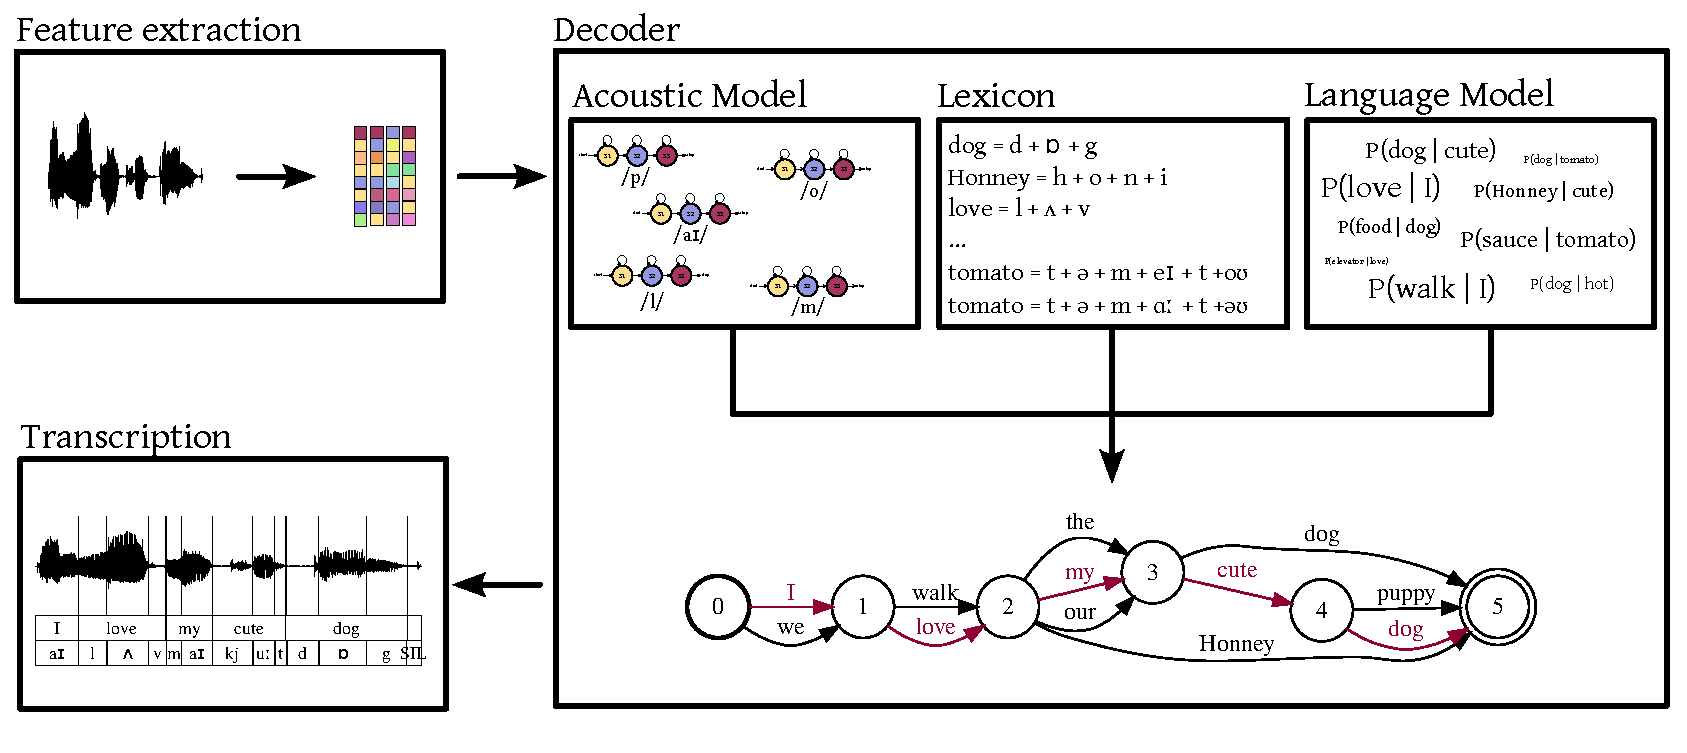
\includegraphics[width=1\linewidth]{chapter03/hmm_all.pdf}
\caption{\textit{Architecture of our ASR system, including its input (acoustic features) and output (transcription).}}
\label{fig:hmm_architecture}
\end{figure}

\subsection{Corpora}

In order to train and test our ASR system, we required transcribed speech corpora. These corpora consisted of speech recordings which have been annotated; for each utterance, we have a more or less detailed transcription of what was said.
While the ideal annotation is one for which phoneticians have provided phoneme categories (or even phones), as well as their boundaries, often we might only have access to by-utterance annotations where we are only provided with a sequence of words/phonemes for each utterance. In these cases, we rely on forced alignment to automatically find phoneme boundaries.

In the following sections we have trained ASR systems with different ``native'' languages, namely Japanese (JP) and Korean (KR). These languages were of particular interest because of their relatively restrictive phonotactic constraints with regards to consonant clusters, as well as the availability of corpora of spontaneous speech, which we will now present. 

\paragraph{Corpus of Spontaneous Japanese (CSJ)}
As the name suggests, the CSJ \cite{maekawa2003} contains recordings of spontaneous Standard Japanese. The corpus is composed of two subparts: (1) academic presentation speech (APS), which consists of live recordings of academic presentations, and (2) simulated public speech (SPS), where speakers presented everyday topics in front of a small audience. For our models we only kept SPS, which is more representative of everyday conversations at the level of the lexicon, and has a more balanced population than the young male-dominated APS.
Our subset of the corpus contained 400,547 utterances produced by 594 speakers (331 female, 263 male), with an average of 674.3 utterances per speaker.  
Recordings were manually transcribed by native speakers of Japanese. Phoneme boundaries were {\color{red}manually adjusted, however this alignment was not used when our models, as it was overwritten by forced alignment}.

\begin{itemize}
{\color{red}\item Train-test division (n utterances, time)}
\end{itemize}

\paragraph{Korean Corpus of Spontaneous Speech (KCSS)}

The KCSS \cite{yun2015} consists of recordings of spontaneous Seoul Korean. Forty speakers aged 10 to 49 (5 female speakers and 5 male speakers per decade) were recorded in a quiet room, for approximately 1 hour each. Speech was ellicited through questions related to the speakers' personal opinions, habits, acquaintances, etc.      
Recordings were manually transcribed by native speakers of Korean. We used phonetic transcriptions faithful to actual pronunciations which, for instance, include phonetic reduction (akin to \textit{yesterday} being transcribed as \textipa{/jESeI/} instead of the canonical \textipa{/jEst\textrhookschwa deI/}). Transcriptions include {\color{red}manually adjusted} phoneme boundaries, as well as word syllabification.
The corpus contains 126,132 utterances produced by 40 speakers (as explained above), with an average of 3153.3 utterances per speaker. 

\begin{itemize}
{\color{red}\item Train-test division (n utterances, time)}
\end{itemize}

\subsection{Features}
In order for our ASR systems to be able to use speech as input, it is necessary to perform signal analysis. This procedure transforms the continuous raw speech waveform into sequential speech features. This latter form ensures a more compact representation of the information in speech, with modifications that enhance phonemic contrasts and better approximate how speech is processed by the human cochlea. In this work we used Mel-frequency cepstrum coefficients (MFCC), traditionally used for HMM-based ASR systems.

\begin{figure}[htb]
\centering
%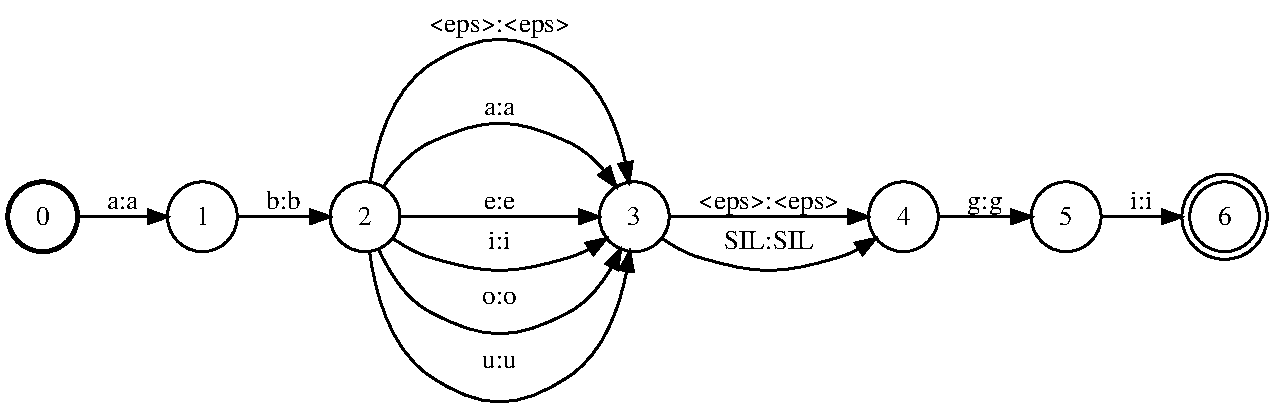
\includegraphics[width=0.8\linewidth]{chapter03/parlato_hmm_Gfst.pdf}
\caption{{\color{red}\textit{[Is this necessary or is the text enough?] Processing stages required to obtain MFCCs.}}}
\label{fig:hmm_architecture}
\end{figure}

Speech is recorded with a microphone; the continuous audio signal is digitalized at a sampling rate of 16kHz.
The audio is then segmented into frames of 25 ms, with a shift of 10 ms between the beginning of each frame. By using frames, we make the assumption that the signal is stationary, and we apply the following proccessing steps to each frame, using Kaldi \cite{povey2011}:

\begin{enumerate}
\item Pre-processing: The data is extracted and pre-processed (dithering, pre-emphasis, and DC offset removal).
\item Windowing: The data in the 25 ms frame is multiplied by a tapered window (Hamming window), to avoid discontinuities at the edges of the segment.
\item Spectral analysis: By applying a Fast Fourier Transform (FFT), we find out how much energy there is at each frequency band.
\item Nonlinear frequency scaling: In order to compensate for the fact that human hearing is less sensitive to higher frequencies, frequencies are mapped onto a Mel scale, which is linear until approximately 1000 Hz and logarithmic afterwards. This is done by applying a mel-filter bank with 23 bins, which are equally spaced in the mel-frequency domain. Each filter summarises the amount of energy in a section of the range of frequencies. 
\item Cepstral analysis: The log of the energy in each bin is computed, from which we take the cosine transform. We keep 13 MFCCs, including $c_{0}$, the zeroth coefficient which represents the average of the log-frequency of the bins \cite{galesyoung2007}..
  \item {\color{red}Cepstral liftering: Coefficients are scaled, ensuring that they have a reasonable range.}
\end{enumerate}

We therefore obtain 13 MFCCs that summarise the information at each frame of audio. To these coefficients, we add 3 coefficients carrying information about pitch: normalized-pitch, delta-pitch, voicing-feature.
To these 16 static features we add their respective dynamic features ($\Delta$ and $\Delta^2$) that describe the evolution of the coefficient values over time. 
Coefficient values are then standardised using Cepstral Mean Variance Normalisation (CMVN); for each speaker the distribution of each coefficient's values has a mean value of zero and a variance of one. 

{\color{red} [TO-DO]: added pitch because better performance for CSJ (+ pitch used in both JP and KR)}

\subsection{Acoustic model}

Now that we have extracted the acoustic features for the labelled utterances in our corpus, we are able to train the acoustic model (AM). Recall that the AM gives the likelihood $P(X|w)$, which corresponds to the probability of the acoustics given the sequence of words $w$.
In order to simplify things, let's not view an utterance as a sequence of words which are sequences of phonemes themselves, but directly as a sequence of phonemes. Then, we consider the probability of the acoustics $X$ given the sequence of phonemes $W$.
Phonemes are not static objects but trajectories of the acoustic signal, of varying duration. By using Hidden Markov Models (HMM), we can approximate these trajectories as sequences of static states. A priori, the more states, the better the approximation. However, empirically it has been assessed that having three states is a good compromise for ASR systems. Following this, we chose to model phonemes as 3-state HMMs, where the states correspond, respectively, to the beginning, middle, and end portions of the phoneme. This is particularly relevant for phonemes that can be viewed as sequences of discrete articulatory events with distinct acoustic signatures, such as plosives (e.g., \textipa{/p/}) which are often described as an airway closure, followed by a period of occlusion and an optional release. Additionally, the separation into three states allows to account for the fact that the acoustics of the beginning and end of a phoneme may be differently affected by neighbouring phonemes (i.e., coarticulation) in comparison to the medial part.

As their name suggests, HMMs follow a Markovian process; the value of a state only depends on the value of the previous state. The transitions between states are defined by transition probabilities not only between adjacent states, but also within a state itself (i.e., self-loops). These transition probabilities are defined during AM training, based on the transitions between frames in the training corpus. While the duration of phonemes cannot be explicitly learned by the acoustic model, they are implicitly reflected by the transition probabilities in the self-loops: for a given state, the higher the self-loop probability, the longer the model will ``remain'' at said state and the longer the sequence of acoustic vectors assigned to the corresponding phoneme. A simplified illustration of a phoneme HMM is shown in Figure \ref{fig:hmm_3state}.

\begin{figure}[htb]
\centering
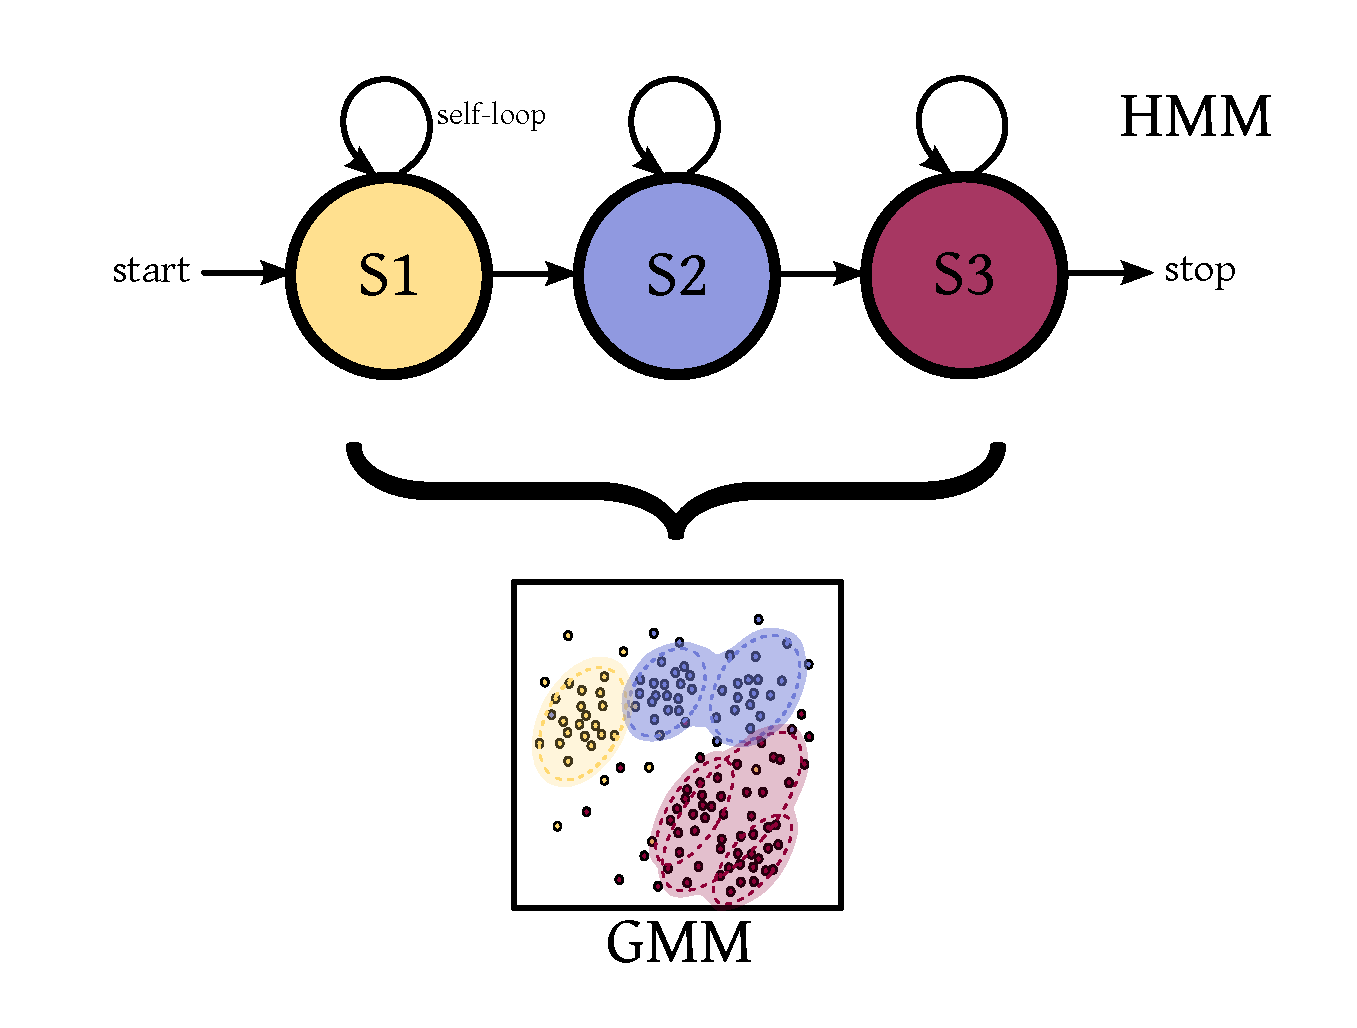
\includegraphics[width=0.6\linewidth]{chapter03/hmm_3state.pdf}
\caption{\textit{Left-to-right 3-state phoneme HMM with simplified 2-dimensional GMMs (one per state). Start and stop states connect the phoneme with the previous and next phoneme, respectively.}}
\label{fig:hmm_3state}
\end{figure}

In sum, each phoneme is modelled by a left-to-right 3-state HMM. But what exactly is a state? Our acoustic models are HMM-GMMs, where GMM stands for Gaussian Mixture Models. For each phoneme our 48-dimensional feature vectors define a 48-dimensional space where GMM for the three states are embedded. During training, the acoustic model will have placed individual acoustic frames on this space, based on the values of their feature vector. In other words, acoustic frames from each phoneme portion will occupy a certain part of this space. For each state, we can parametrically define the space covered using mixtures of Gaussian distributions (the aforementioned GMMs). Indeed, GMMs are universal approximators of densities when given enough components. To do this, the model will have fitted a number of diagonal Gaussian distributions to approximate the distribution of datapoints corresponding to each phoneme state. The number of Gaussians allocated to each phoneme state depends on the total number of Gaussians made available to the model, and the complexity of the distribution of the frames in the space. Once that the GMMs are defined, the AM is able to tell us, for any new frame, the likelihood that the frame originated from each GMM (i.e., phoneme state).  \\     


{\color{red} $<$OLD VERSION$>$
\subsubsection{Estimating Gaussian distributions}
We have 48-dimensional vectors (i.e., our acoustic features), as well as their accompanying transcriptions, as input for our acoustic model. As such, for each acoustic frame, we know the identity of the phoneme that it constitutes. Therefore, we have access to a variety of feature vectors which we can group by phonemic category. Using these distributions of acoustic vectors, we are able to represent each phoneme as a multivariate Gaussian distribution with 48 dimensions. During training, our acoustic model learns what each multivariate Gaussian distribution looks like for each phoneme by estimating the means and covariance matrices necessary for defining said distributions.
Then, the AM is able to tell us, for any new frame $x$, $P(x|w_{l})$ the likelihood that the frame originates from each multivariate distribution (i.e., phoneme) $w_{l}$. However, this assumes that a (multivariate) Gaussian distribution will be sufficient to model the distribution of our data. This is a strong assumption but it is made unnecessary by replacing multivariate Gaussian distributions with Gaussian Mixture Models (GMM).

\subsubsection{Adding Gaussian Mixture Models (GMM) into the mix}
Indeed, given enough components, GMMs are universal approximators of densities. We can therefore represent each phoneme not as a single multivariate Gaussian but as a mixture of multiple ones, relaxing the normality assumption. Similar to the single multivariate case, training consists of teaching the acoustic model what the distribution of exemplars of each phoneme looks like. The AM can then fit mixtures of Gaussians to fit these (non-Gaussian) distributions. When presented with a new frame, the AM can retrieve the likelihood that it originates from each GMM (i.e., phoneme). However, this type of acoustic model does not take into consideration the sequential nature of speech. Here is where Hidden Markov Models (HMM) come into place.   

\subsubsection{Modelling sequences with HMMs}
Before even mentioning how different phonemes are connected to each other in HMMs, our first modification will be within the representation of an individual phoneme itself. While in the previous paragraph each phoneme was a GMM, now we represent a phoneme by a sequence of three GMMs, called \textbf{states}. In a left-to-right model such as ours, the three states are disposed sequentially (i.e., it is only possible to go from state 1 to state 2, and from state 2 to state 3) and they correspond to a description of phonemes unfolded in the time domain. Shifting to a three-state representation allows us to better handle the variability in phoneme production due to coarticulation; indeed, while state 2 represents the more stable, medial portion of a phoneme, states 1 and 3 will be subjected to more diversity due to surrounding phonemes. Additionally, some phonemes are better represented by a sequence of steps rather than a stationary description of their acoustics. For instance, plosives such as \textipa{/p/} are often described as sequences of an airway closure, followed by a period of occlusion and an optional release.

In previous paragraphs we mentioned that, during training, our AM was learning the GMMs for all phonemes based on the corpus data. Now that we represent phonemes as three-state HMMs, our AM also needs to learn the transition probabilities, within states (i.e., self-loops) and between adjacent states. How do we go from isolated phonemes to sequences of phonemes? Phoneme HMMs are simply chained together, meaning that the AM also learns the transition probabilities between the last state and first state of a pair of phonemes.

Please note that HMMs follow a Markovian process; the probability of a state only depends on the state beforehand. Consequently, the duration of phonemes cannot be explicitly learned by the acoustic model. However, durations are implicitly reflected by the transition probabilities in the self-loops: for a given state, the higher the self-loop probability, the longer the model will ``remain'' at said state and the longer the sequence of acoustic vectors assigned to the corresponding phoneme.  \\
$<$/OLD VERSION$>$}

\subsubsection{Why not triphones?}
If the reader is already familiar with ASR systems, they may expect us to go a step further and no longer treat phonemes as units (i.e., monophones) but, instead, handle triphones. For this latter representation, an independent three-state HMM would be built for each combination ofthree phonemes. For instance, there would no longer be an HMM for \textipa{/p/}, but we would have all context-dependent versions of this phoneme as individual HMMs (e.g., the triphone \textipa{/a+p+i/}, which is the phone \textipa{/p/} when preceded by \textipa{/a/} and followed by \textipa{/i/}).
Traditionally, triphone-based HMM-based ASR systems perform better than monophone systems. However, this does not apply to our situation. Recall that we aim to use these speech recognition systems as models of nonnative speech perception, using tasks analogous to paradigms used in psycholinguistic experiments (namely, identification/forced-choice tasks). Importantly, we are focusing on modelling perceptual vowel epenthesis. This context excludes the use of triphones for the following reasons:
\begin{enumerate}
\item First of all, by definition, our ASR systems will have to decode speech that does not follow native phonotactics. Decoding such stimuli requires the existence of triphones corresponding to the input, yet the model will have never encountered such triphones in the training data. While this situation might seem appealing, one must consider the fact that the ASR system \textit{will attempt to account for said triphones} during decoding in spite of the lack of data. Importantly, poorly estimated triphones (e.g., \textipa{/a+h+p/}, when decoding \textipa{/ahpa/}) will be put up against well-estimated triphones (e.g., \textipa{/a+h+a/}) during the forced-choice tasks. The well-estimated triphones might simply be preferred as transcriptions over poorly-estimated ones for this reason alone, irrespective of the actual acoustic match between the stimuli and the phoneme models.
  \item Secondly, our tasks consist of phonetic labelling. It has been shown that monophone models are able to perform well in this context relative to triphones, as long as the number of Gaussians available to the model is increased {\color{red}\cite{saraclar2001}}. As shown in Figure \ref{fig:hmm_gaussians}, the performance of our models increased when increasing the number of total Gaussians from the Kaldi default of 1000 to 6000, which would average to approximately 50 Gaussians per state for a language with an inventory of 40 phonemes.   
\end{enumerate}

\begin{figure}[htb]
\centering
%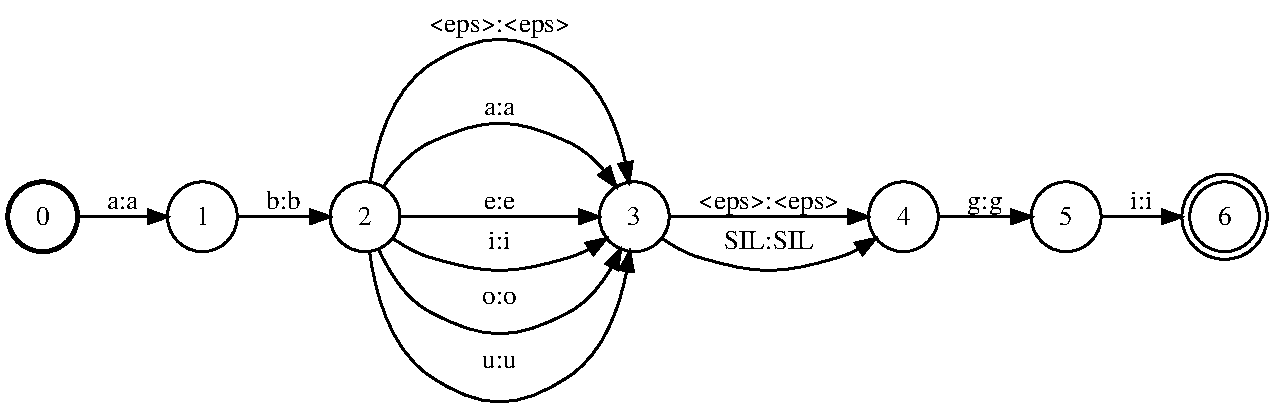
\includegraphics[width=0.8\linewidth]{chapter03/parlato_hmm_Gfst.pdf}
\caption{{\color{red}\textit{Changes in word error rate (\%WER) and phone error rate (\%PER) following variation of the number of total Gaussians allocated to the acoustic model.}}}
\label{fig:hmm_gaussians}
\end{figure}

\subsection{Language models}
\begin{itemize}
\item WFSTs
\item Words \& phones 
\item n-grams
\item ...
\end{itemize}

\subsection{Decoding}
\begin{itemize}
\item Lattice generation
\item Acoustic and LM scores 
\item nbest
\item CTM
\item ...
\end{itemize}

\subsection{Scoring: Assessing native performance}
\begin{itemize}
\item Lexicon-based decoding
\item Phonetic-based decoding
\end{itemize}

%%%%%%%%%%%%
% Parlato2 %
%%%%%%%%%%%%
\newpage
\section{{\color{red}Parlato-hmm}} \label{3-parlato-hmm}
\subsection{Introduction}
\subsection{Methods}
\subsubsection{Stimuli}
We used the same stimuli as in sections \ref{2-parlato} and \ref{2-parlato-dur}. As a reminder, a native French speaker recorded 54 items with the structure $V_{1}C_{1}C_{2}V_{2}$, with $V_{1}$ and $V_{2}$ vowels from the set \{/a/, /i/, /u/\}, and $C_{1}C_{2}$ a cluster from the set \{/bg/, /bn/, /db/, /dg/, /gb/, /gn/\} (e.g. /abgi/).

\subsubsection{Language models}
In order for the decoding task to be analogous to the experiment described in sections \ref{2-parlato_per} and \ref{2-parlato-dur}, trial-specific language models were constructed, as shown in Figure \ref{fig:parlato_G}. Thus, when decoding a $V_{1}C_{1}C_{2}V_{2}$ stimulus, the perception model was only given the possibility to transcribe it as $V_{1}C_{1}(V_{3})(SIL)C_{2}V_{2}$, where phones between parentheses are optional and $V_{3}$ was from the set of vowels \textipa{/a, e, i, o, u/}. In this section our language model was only used to constrain the list of possible outputs from decoding; one output was not more probable than another based on the language models alone. Therefore, here we used a null language model, meaning that the quality of the epenthesized vowels was only determined by the acoustic match.

\begin{figure}[htb]
\centering
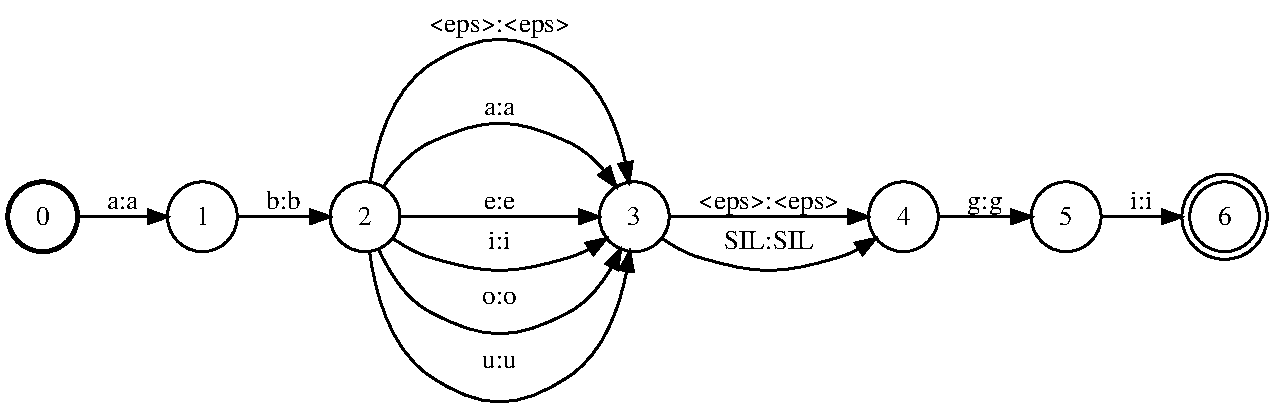
\includegraphics[width=0.8\linewidth]{chapter03/parlato_hmm_Gfst.pdf}
\caption{Constrained language model used for decoding the stimulus \textipa{/agni/}. Nodes in the graph represent states, edges represent transitions between states (here: phonemes). The lack of weights on edges issued from a same node (e.g., between states 2 and 3) indicates that path selection is entirely decided by acoustic scores when decoding experimental items, with an acoustic scale of $0.1$. An optional silence can be inserted by the model between states 3 and 4.}
\label{fig:parlato_G}
\end{figure}

\subsubsection{Identification task simulation}
After decoding the stimuli, we obtained for each possible transcription of each item the corresponding acoustic and language model scores. An example of how the ASR system decodes the experimental stimuli can be seen in Figure \ref{fig:parl_hmm_align}. From the acoustic and language model scores\footnote{with an acoustic scale of $0.1$} we derived the item posteriorgrams, which indicate how probable a given transcription was given the audio input. We used these probabilities as proxies of the probability that a listener might exploit when performing reverse inference during speech perception, and therefore, the probabilities used when responding in an identification task. 

As such, for each item, we obtained a six-dimensional vector $ident_{model} = [p_{none}, p_{a}, p_{e}, p_{i}, p_{o}, p_{u}]$, containing a discrete probability distribution, with a probability mass function linking the identification task options `none', `a', `e', `i', `o', `u', to their respective probabilities (i.e., posteriorgrams).
We can define the human equivalent $ident_{human} = [p_{none}, p_{a}, p_{e}, p_{i}, p_{o}, p_{u}]$, which contains the percentage of responses for each item, after aggregating all participant responses. 

\begin{figure}[htb!]
  \centering
  \begin{overpic}[trim={0 2.5cm 0 1.5cm},clip, width=0.8\linewidth]{chapter03/parlato-hmm_praat_agni.pdf}\end{overpic}
  \caption{\textit{Example of how the ASR system decodes the item \textipa{/agni/}, using the null language model in Figure \ref{fig:parlato_G}. From top to bottom: original waveform, item name, aligned transcriptions given by the model (from the most probable to the least probable), and spectrogram with formant contours. SIL = silence.}}
  \label{fig:parl_hmm_align}
\end{figure}

\subsubsection{Data analysis}
Statistical analyses were performed with the R statistical software \cite{R-base}, using Markov chain Monte Carlo generalised linear mixed-models \cite{R-MCMCglmm, R-coda}. These Bayesian models sample coefficients from the posterior probability distribution conditioned on the data and given priors. We used priors that are standard for linear models. Model convergence was assessed by visual inspection of trace plots and the Gelman–Rubin convergence diagnostic \cite{gelman1992}, using eight chains with different initialisations. Effects were considered statistically significant if the 95\% highest posterior density (HPD) interval estimated for the coefficient of interest did not include zero. We report both the posterior mode and the 95\% HPD interval.  

In order to assess the influence of $V_{1}$ and $V_{2}$ (henceforth: flanking vowels) on epenthetic vowel quality (/i/ or /u/), we chose as fixed effect for our statistical models \textsc{Number of Same Flanking Vowels} (\textsc{NSFV}; considered as a continuous variable with values 0, 1, or 2 instead of a factor with 3 levels, in order to reduce the number of model parameters and promote convergence). Due to the almost null variance and the consequent poor trace plot for the random intercept \textsc{Cluster}, we did not include it in the statistical models. Our response variable was the continuous variable \textsc{Posteriorgram}.\footnote{Responses by human participants and exemplar models were given by trial; therefore in previous analyses the response variable was binomial.}

\subsection{Results}
\subsubsection{Overall similarity}
\begin{figure}[H]
  \centering
  \begin{overpic}[trim={0 0 0 0.75cm}, clip, page=1, width=0.5\linewidth]{chapter03/parl_hmm_figs}\end{overpic}
  \caption{\textit{Distribution of posteriorgrams obtained when decoding with a null language model. The box and whiskers plots display the distribution of posteriorgrams across experimental items.}}
  \label{fig:parl_hmm_overall}
\end{figure}
Figure \ref{fig:parl_hmm_overall} shows the distribution of posteriorgrams for each response, with one datapoint per stimulus. The most probable transcriptions for the stimuli were ``none'' (26.7\%), ``u'' (24.3\%) and ``i'' (22.5\%).  While these were also the most frequent responses given by human participants (``none'': 13.1\%; ``u'': 63.1\%; ``i'': 15.3\%), the preponderance of \textipa{/u/}-epenthesis is missing in the model.

% > agr.ep (model average pgram)
%   resp          x
% 1 none 0.26667043
% 2    a 0.04802057
% 3    e 0.12948173
% 4    i 0.22494707
% 5    o 0.08715853
% 6    u 0.24372167

% > colMeans(d.comp.per[-1]) (human average resp)
%     p.none        p.a        p.e        p.i        p.o        p.u 
% 0.13071895 0.01416122 0.02505447 0.15250545 0.04684096 0.63071895 

In order to have a general idea of the model's ability to reproduce human behaviour, we computed the distance between human and model response patterns by computing the normalized Euclidean distance between $ident_{model}$ and $ident_{human}$, within each experimental item. The mean (and median) distance was $0.44$. This is higher than what was obtained by the best exemplar model in section \ref{2-parlato-dur} (mean distance: $0.33$; median distance: $0.21$); however remember that exemplar models were only able to output ``i'', ``o'', and ``u'' as responses. When computing the distance by taking into account the missing responses ``none'', ``a'', and ``e'', responses from the best JP exemplar model have a mean distance of $0.39$ (median: $0.30$) with respect to human responses.

While it might be tempting to conclude that the exemplar model was superior compared to the HMM model, it is important to note that the task modelled by the HMM-based model is closer to the task participants were subjected to (6-alternative forced choice identification task) than the exemplar models (3-AFC identification task). Technically, a ``dummy'' model in the 3-AFC situation, where all options are equally probable, would output ``u'' for $33\%$ of the trials. This is a higher percentage of \textipa{/u/}-epenthesis than the $24.3\%$ from our current model. Since ``u'' is by far the most frequent response given by human participants (and ``a'' and ``e'' are very infrequent), even a dummy 3-AFC \textipa{\{``i'', ``o'', ``u''\}} model might outclass our 6-AFC \textipa{\{``none'', ``a'', ``e'', ``i'', ``o'', ``u''\}} ASR system.

As such, we believe that it is unfair to compare Euclidean distances between models based on different tasks. We can, however, see if the ASR-based model reproduces the qualitative effects that the best exemplar model was able to mimic.

\subsubsection{Effect of coarticulation}

\paragraph{/i/-epenthesis}

The left panel of Figure \ref{fig:parl_hmm_iu} shows the posteriorgrams for \textipa{/i/}-epenthesis given by our ASR-based model with a ``null'' language model.
The main effect of \textsc{NSFV} was significant (mode: $0.10$, HPD: $[0.01, 0.18]$). An increased number of \textipa{/i/} flanking vowels resulted in higher posteriorgrams for stimuli transcriptions with \textipa{/i/} epenthesis.

\begin{figure}[H]
  \centering
  \begin{overpic}[page=2, width=0.4\linewidth]{chapter03/parl_hmm_figs}\end{overpic}
  \hspace{1cm}
  \begin{overpic}[page=3, width=0.4\linewidth]{chapter03/parl_hmm_figs}\end{overpic}
  \caption{\textit{Posteriorgrams for \textipa{/i/}-epenthesis (left) and \textipa{/u/}-epenthesis (right) obtained when decoding with a ``null'' language model. The box and whiskers plots display the distribution of posteriorgrams across experimental items, represented by individual dots.}}
  \label{fig:parl_hmm_iu}
\end{figure}

\paragraph{/u/-epenthesis}
The right panel of Figure \ref{fig:parl_hmm_iu} shows the posteriorgrams for \textipa{/u/}-epenthesis given by our ASR-based model with a ``null'' language model.
The main effect of \textsc{NSFV} was not significant (mode: $0.04$, HPD: $[-0.02, 0.10]$). Therefore, an increased number of \textipa{/u/} flanking vowels did not result in significantly higher posteriorgrams for stimuli transcriptions with \textipa{/u/} epenthesis.

\subsection{Discussion}
%%% Summary

%%% Duration in ASR? [check topology]

%%%%%%%%%%%%%%%%%%%%%%%%%%
% m-/ahpa/ + parlato_lms %
%%%%%%%%%%%%%%%%%%%%%%%%%%
\newpage
\section{{\color{red}Investigating surface phonotactics}} \label{3-surfphono}

\small{\textit{{\color{red}ADD ACKNOWLEDGEMENTS THOMAS + EMMANUEL.\\}}}

\subsection{Introduction}
\subsection{Experiment 1: {\color{red}Parlato-lms}}
\subsubsection{Methods}
\paragraph{Stimuli}
We used the same stimuli as in sections \ref{2-parlato}, \ref{2-parlato-dur}, and \ref{3-parlato-hmm}. As a reminder, a native French speaker recorded 54 items with the structure $V_{1}C_{1}C_{2}V_{2}$, with $V_{1}$ and $V_{2}$ vowels from the set \{/a/, /i/, /u/\}, and $C_{1}C_{2}$ a cluster from the set \{/bg/, /bn/, /db/, /dg/, /gb/, /gn/\} (e.g. /abgi/).

\paragraph{Language models}
In this section, we investigate the type of phonotactic information that might be used by Japanese listeners when perceiving foreign speech that does not conform to native phonotactics. We test 5 types of language models (LM) when decoding our $V_{1}C_{1}C_{2}V_{2}$ items; these differ only in the weights given to edges between nodes 2 and 3 in the graph shown in Figure \ref{fig:parlato_G}. 
\begin{enumerate}
    \item A null language model, which implies that listeners base their decoding of consonant clusters on phonetics alone, without using information on phonotactics (as in section \ref{3-parlato-hmm}).
    \item A phone-unigram language model, which implies that listeners do not take neighbouring phonemes into consideration when decoding the consonant clusters; only the frequency of the vowel $V_{ep}$ to be epenthesized (compared to that of $C_{2}$) is taken into account when choosing epenthetic vowel quality.
    \item An online phone-bigram language model, which implies that listeners decode the clusters as they hear them (decoding is done from the start of the item). Here the choice of epenthetic vowel is modulated by $C_{1}V_{ep}$ and $C_{1}C_{2}$ diphone frequencies. 
    \item A retro phone-bigram language model, which implies that listeners decode the clusters based on the most recent information (decoding is done from the end of the item). Here the choice of epenthetic vowel is modulated by $V_{ep}C_{2}$ and $C_{1}C_{2}$ diphone frequencies.
    \item A batch phone-bigram language model, which implies that listeners decode the item considering the entire structure, with bigrams. Here the choice of epenthetic vowel is modulated by $C_{1}V_{ep}$ and $V_{ep}C_{2}$ (and $C_{1}C_{2}$) diphone frequencies.  
\end{enumerate}

The weights, which can be found in Table \ref{}, were obtained by taking frequency counts from the portion of the CSJ used for training the acoustic model: 
{\color{red}ADD TABLE WITH FREQUENCIES}


\paragraph{Identification task simulation}
We used the same procedure as in section \ref{3-parlato-hmm}. Therefore, for each LM, we obtain for each item a six-dimensional vector $ident_{LM} = [p_{none}, p_{a}, p_{e}, p_{i}, p_{o}, p_{u}]$ containing posteriorgrams for each of the six possible responses. In a similar way, the human equivalent $ident_{human} = [p_{none}, p_{a}, p_{e}, p_{i}, p_{o}, p_{u}]$ contains the percentage of responses for each item, after aggregating all participant responses. 

\paragraph{Data analysis}
In order to compare how well LMs compared at mimicking human behaviour, we computed the Euclidean distance between $ident_{LM}$ and $ident_{human}$ for each item, for each LM. Do models that integrate information about phoneme probabilities (i.e., \textsc{unigram} LM) or diphone probabilities (i.e., \textsc{bigram} LMs) show smaller \textsc{Eucl. distances} to human data than the \textsc{null} LM?

The response variable of our statistical models was the \textsc{Eucl. distance} between $ident_{LM}$ and $ident_{human}$, as described above.  
We chose as fixed effect the \textsc{Language Model} (\textsc{LM}) used during decoding, considered as a categorical variable with \textsc{null} as the reference level. The variable was contrast coded with simple coding, meaning that non-reference levels were compared to the reference level, with the intercept corresponding to the grand mean (all levels).
\textsc{$C_{1}$} was added as a random intercept.

Statistical analyses were performed with the R statistical software \cite{R-base}, using Markov chain Monte Carlo generalised linear mixed-models \cite{R-MCMCglmm, R-coda}. These Bayesian models sample coefficients from the posterior probability distribution conditioned on the data and given priors. We used priors that are standard for linear models. Model convergence was assessed by visual inspection of trace plots and the Gelman–Rubin convergence diagnostic \cite{gelman1992}, using eight chains with different initialisations. Effects were considered statistically significant if the 95\% highest posterior density (HPD) interval estimated for the coefficient of interest did not include zero. We report both the posterior mode and the 95\% HPD interval.  

%\begin{itemize}
%\item \textsc{\%none}: Proportion of ``none'' responses (no epenthesis) over all trials.
%\item \textsc{\%$V_{1}\underline{\vee}V_{2}$}: Proportion of trials where the epenthesized vowel shares the quality of either $V_{1}$ or $V_{2}$, with $V_{1} \neq V_{2}$ (out of all trials with epenthesis).
%\item \textsc{\%$V_{1}\land V_{2}$}: Proportion of trials where the epenthesized vowel shares the quality of both $V_{1}$ and $V_{2}$, with $V_{1} = V_{2}$ (out of all trials with epenthesis).
%\item \textsc{\%default}: Proportion of default \textipa{/u/}-epenthesis over all trials
%\item \textsc{\%coronal}: Proportion of \textipa{/o/}-epenthesis following coronal consonants over all trials with clusters containing coronal consonants 
%\end{itemize} 

\subsubsection{Results and Discussion}
\begin{figure}[htb!]
    \centering
    \includegraphics[page=2, width=0.8\linewidth]{chapter03/parlato-lms_figs.pdf}
    \caption{\textit{Distribution of the proportion of responses given by human participants (topmost panel) and posteriorgrams obtained when decoding with different language models. The box and whiskers plots display the distribution of posteriorgrams across experimental items, with boxplots separated according to the $C_{1}$ in the cluster.}}
    \label{fig:parlato-lms}
  \end{figure}
  
\paragraph{Effect of acoustic scale}

\paragraph{Response patterns}
{\color{red}Graph showing response patterns}


\paragraph{Overall similarity}
We found that, relative to the \textsc{null} LM, the \textsc{bigram online} (mode: $0.08$, HPD: $[0.02, 0.15]$) and the \textsc{bigram batch} (mode: $0.08$, HPD: $[0.02, 0.15]$) language models resulted in significantly higher Euclidean distances between the model responses and human responses. On the other hand, we did not find evidence of a difference between the \textsc{null} LM and the \textsc{unigram} (mode: $0.03$, HPD: $[-0.04, 0.10]$) or \textsc{bigram retro} (mode: $0.0$, HPD: $[-0.06, 0.07]$) language models.

\paragraph{Zooming in on epenthetic vowel quality}
We arbitrarily chose a smoothing factor ($10^{-8}$)  in order to allow the language models to assign a non-zero probability to diphones never seen in the language corpus. The magnitude of this smoothing factor is expected to have an effect on the posteriorgrams assigned to ``none'' responses when decoding the experimental items. Since ``none'' responses constitute $13\%$ of human responses, and since the choice of the smoothing factor only affects the bigram language models, it may be beneficial to do a post-hoc analysis focusing on the models' ability to mimic epenthetic vowel quality after isolating it from the percentage of epenthesis. As such, we perform the same analysis as above, but after removing $p_{none}$ from $ident_{LM}$ and $ident_{human}$.

The results are qualitatively identical: relative to the \textsc{null} LM, only the \textsc{bigram online} (mode: $0.11$, HPD: $[0.05, 0.19]$) and the \textsc{bigram batch (2PB)} (mode: $0.11$, HPD: $[0.05, 0.19]$) language models resulted in significantly higher Euclidean distances. There was no evidence of a significant difference for the \textsc{unigram (1P)} (mode: $0.06$, HPD: $[-0.02, 0.12]$) or \textsc{bigram retro (2PR)} (mode: $0.03$, HPD: $[-0.04, 0.10]$) language models 

Interestingly, the models that performed less similarly to human behaviour are those for which \textipa{/u/}- and \textipa{/i/}-epenthesis was blocked after coronal consonants, since \textipa{/du/} and \textipa{/di/} are phonotactically illegal in Japanese and therefore do not appear in our corpus. Yet, as seen in Figure \ref{fig:parlato_per_all}, JP participants mostly reported experiencing \textipa{/u/}- and \textipa{/i/}-epenthesis on trials where $C_{1}$ was a coronal consonant. Similar to how ``none'' responses are blocked for all bigram models, acoustics are unable to counter the low diphone probability of \textipa{/du/} and \textipa{/di/}.

\subsection{Experiment 2: {\color{red}m-/ahpa/}}
\subsubsection{Methods}
\paragraph{Stimuli}
We used the same stimuli as in section \ref{2-ahpa}. As a reminder, we recorded 3 speakers producing disyllabic $V_{1}C_{1}C_{2}V_{1}$ and trisyllabic $V_{1}C_{1}V_{2}C_{2}V_{1}$, with $V_{1}$ a flanking vowel in the set \textipa{/a, e, i, o, u/}, $C_{1}$ \textipa{/h/} or /k/, and $C_{2}$ a fixed consonant, /p/ (e.g, \textipa{/ahpa/}, \textipa{/ahapa/}). By cross-splicing the disyllabic natural control items (e.g., \textipa{/ahpa/}), we obtained disyllabic spliced control items (e.g., \texorpdfstring{\textipa{/ah\textsubscript{a}pa/}}{}), disyllabic spliced test stimuli (e.g., \texorpdfstring{\textipa{/ah\textsubscript{u}pa/}}{}), and trisyllabic spliced fillers (e.g., {\textipa{/ahapa/}), where subscripts indicate the identity of the vowels flanking the clusters in the original recording. Therefore, within each speaker, all stimuli of the same structure (in our example, \textipa{/ah($V$)pa/} items) are acoustically identical on their flanking vowels.
  
\paragraph{Language models}
We used the same language models as in Experiment 1, adapted to the $V_{1}C_{1}C_{2}V_{1}$ items used in this experiment. A graphical representation can be found in Figure \ref{fig:m-ahpa_G}.
  
\begin{figure}[htb]
    \centering
    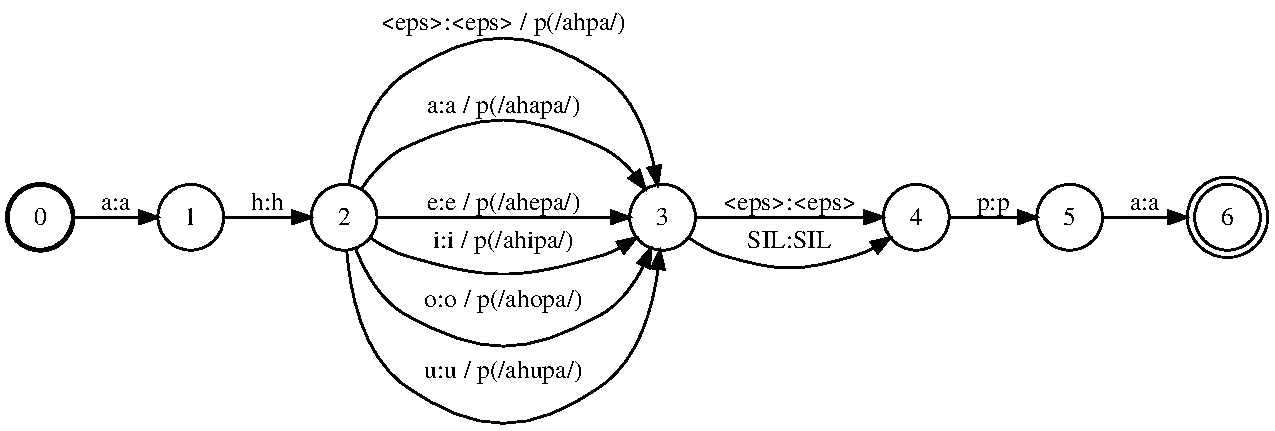
\includegraphics[width=0.8\linewidth]{chapter03/m-ahpa_Gfst.pdf}
    \caption{\textit{Constrained language model used to test the models (here: LM for \textipa{/ahpa/} trials). Nodes in the graph represent states, weighted edges represent transitions between states (here: phonemes). When relevant, weighted edges are labeled with the probability to choose that edge when decoding, which affects the final language model score of each possible path. These scores are then combined with acoustic scores when decoding experimental items.}}
    \label{fig:m-ahpa_G}
\end{figure}
  
\paragraph{Identification task simulation}
We used the same procedure as in section \ref{3-parlato-hmm}.

\paragraph{{\color{red}Data analysis}}
% Refer to previous experiment
% Model selection
% Parameter tuning

%In order to select the language model which best predicted our behavioural data, we inferred the \textit{a posteriori} distributions of the weights given to acoustic model and language model in {\color{red}equation \ref{}}, using ABC. The following aggregated data were used as summary statistics:

%\begin{itemize}
%\item \textsc{\%none}: Proportion of ``none'' responses (no epenthesis)
%\item \textsc{\%coart}: Proportion of trials where the epenthesized vowel shares the quality of the coarticulation within the consonant (including \textipa{/u/} coarticulation).
%\item \textsc{\%default}: Proportion of default \textipa{/u/}-epenthesis over all trials
%\end{itemize}

%Since we saw in section \ref{2-ahpa} that patterns of epenthesis differed depending on whether the consonant cluster was \textipa{/hp/} or \textipa{/kp/}, we computed these summary statistics twice, one set per consonant cluster. As such, the final number of statistics was six. 

\subsubsection{Results and Discussion}
\subsection{Discussion}

%%%%%%%%%%%%
% k-epenth %
%%%%%%%%%%%%
\newpage
\section{{\color{red}Do we need to go deeper? Are surface phonotactics enough?}} \label{3-k-epenth}
\subsection{Introduction}
\subsection{Methods}
\subsubsection{Stimuli}

The stimuli, which have been previously used in \cite{durvasula2015}, were kindly provided by the authors from said paper. They consist of 12 items of the form \textipa{/e}C(V)\textipa{ma/}, with \textsc{C} either an alveolar consonant from the set \{\textipa{/t\super h, s/}\} or a palatal consonant from the set \{\textipa{c\super h, S/}\}, and \textsc{V} a vowel from the set \{\textipa{/1}\footnote{Following the original article, we use \textipa{[1]} to denote the close back unrounded vowel. However, the notation \textipa{[W]} has also previously been used (e.g., in \cite{kabak2007})}\textipa{, i/}\}.
Each item was recorded twice by a male trained phonetician. The speaker is a native speaker of Indian English and Telugu, also a near-native speaker of standard Hindi. The clusters present in the items are phonotactically legal in these two latter languages. All items were produced with stress on the first syllable.
The organisation of the stimuli, based on place of articulation of \textsc{C}, is shown on Table \ref{tab:k-ep_stim}.

\begin{table}[htb!]
\centering
\caption{\textit{Experimental items. Reproduced from \cite{durvasula2015} (Table I).}}
\label{tab:k-ep_stim}
\begin{tabular}{c|c|c|c|c}
  \cline{2-4}
         & \multicolumn{3}{c|}{vowels} &  \\ \cline{2-4}
         & \textipa{[1]}         & \textipa{[i]}    & none    &  \\ \cline{1-4}
  \multicolumn{1}{|l|}{alveolar} & \textipa{et\super h1ma}     &  \textipa{et\super hima}    &  \textipa{et\super hma}       &  \\ \cline{2-4}
  \multicolumn{1}{|l|}{}       &  \textipa{es1ma}         &  \textipa{esima}    &  \textipa{esma}       &  \\ \cline{1-4}
  \multicolumn{1}{|l|}{palatal}  &  \textipa{ec\super h1ma}          &  \textipa{ec\super hima}     &  \textipa{ec\super hma}        &  \\ \cline{2-4}
  \multicolumn{1}{|l|}{}                       &  \textipa{eS1ma}         &  \textipa{eSima}    &  \textipa{eSma}       & \\ \cline{1-4} 
\end{tabular}
\end{table}

\paragraph{Language models}

\paragraph{Identification task simulation}


\subsubsection{Data analysis}
\subsection{Results}
\subsection{Discussion}
%%%%%%%%%%%%%%%%%%%%%%%%%%%
% Chapter mini-discussion %
%%%%%%%%%%%%%%%%%%%%%%%%%%%
\section{Conclusions}
%%% Summary

%%% Short discussion

%%% Limitations

%%% Conclusions
\chapter{Conclusion}
\paragraph{Paradigm}
\begin{itemize}
  \item Identification task -> metalinguistic. How to model A(B)X task with our models?
  \end{itemize}

\paragraph{ASR system}
\begin{itemize}
\item Native performance not state-of-the-art. Influence on results?
\item Influence of using forced-alignment instead of manual alignments?
  \item Input features?
  \end{itemize}

  
%%% ASR system
%% - 

%\chapter{References}
\bibliographystyle{apalike}
\bibliography{main}

\appendix
\fancyhead{}
%\fancyhead[RO, LE]{\rightmark}
\fancyhead[RO,LE]{\nouppercase{\leftmark}}
\fancyfoot{}
\fancyfoot[LE,RO]{\thepage}
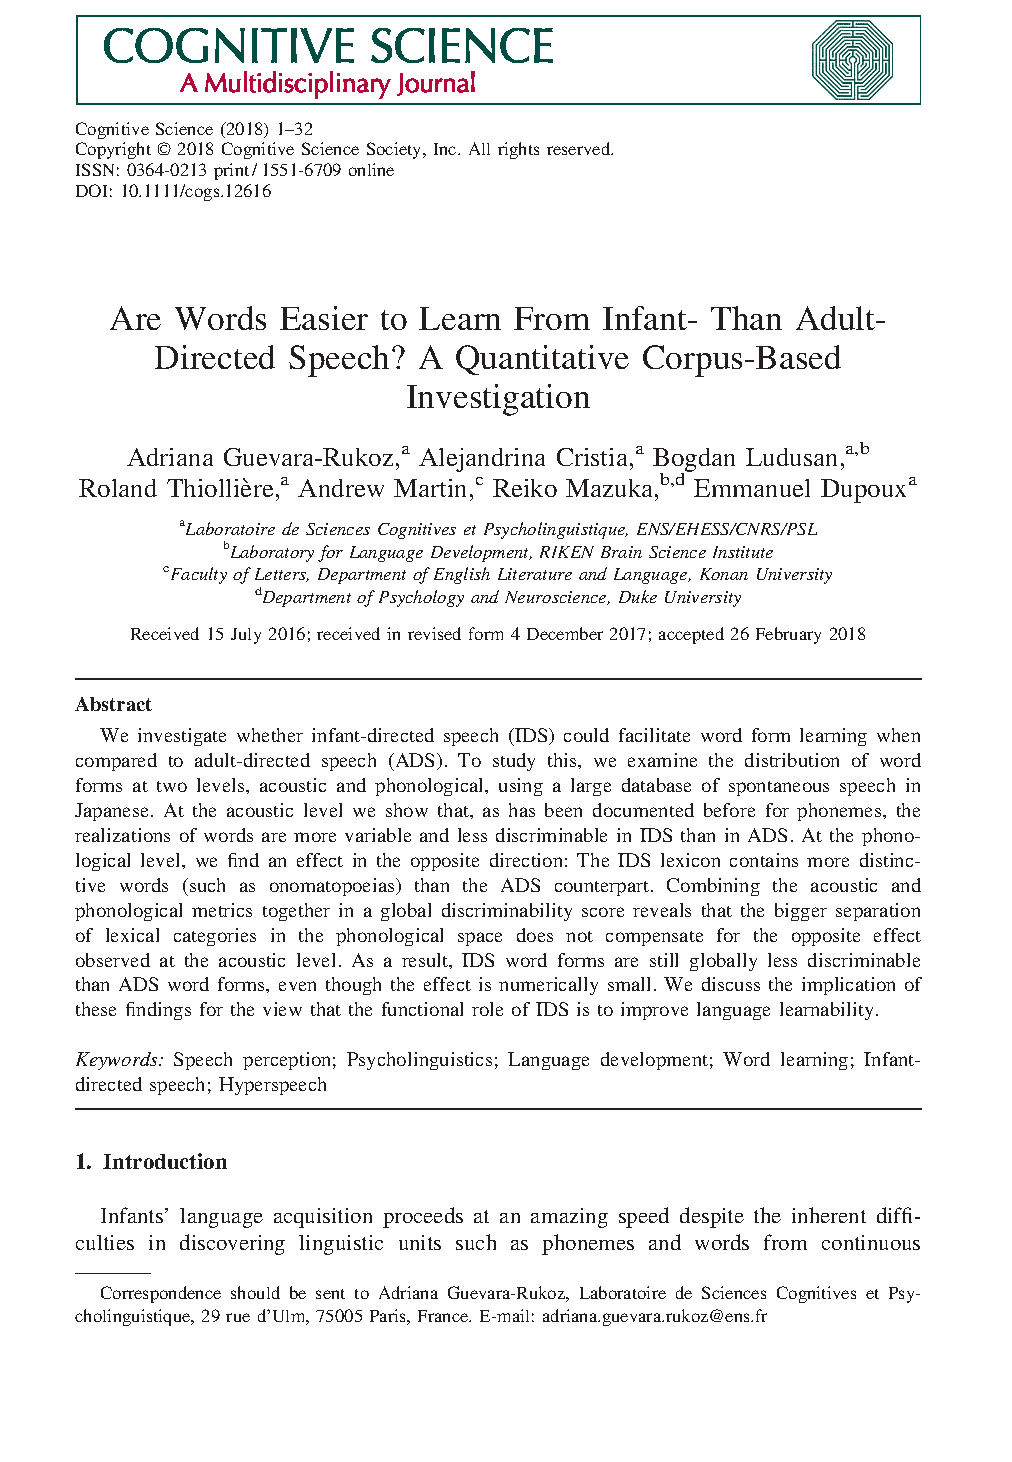
\includepdf[pages={-},pagecommand={},
        addtotoc={1,chapter,1,Are words easier to learn from infant- than adult-directed speech? A quantitative corpus-based investigation, RIKENlex}]
{images/appendix/IDS_ADS_Riken_word_cogsci2018.pdf}
%{images/appendix/IDS_ADS_Riken_word_discriminability_20171227_draft.pdf}


 %% [TODO]: Add to table of contents

\end{document}

%%%% TO-DO %%%%
% Fix references (apa-like + \citeNP etc)
